\documentclass[12pt,a4paper]{article}
\usepackage[utf8]{inputenc}
\usepackage[german]{babel}
\usepackage[T1]{fontenc}
\usepackage{amsmath}
\usepackage{amsfonts}
\usepackage{amssymb}
\usepackage{graphicx}
\usepackage[left=2.5cm,right=2.5cm,top=2cm,bottom=2cm]{geometry}
\author{Gruppe C14 \\ Julián Häck, Martin Koytek, Lars Wenning, Erik Zimmermann}
\title{Akustik}
\usepackage{float}
\begin{document}
\maketitle
\newpage
\tableofcontents
\newpage
\section{Bestimmung der Schallgeschwindigkeit durch Laufzeitmessung}
\subsection{Versuchsbeschreibung}
%Kurze Darstellung der physikalischen Grundlagen und Ziele der Versuche, %die zum Verständnis
%des Versuches/Protokolls benötigt werden. (max. 1 Seite)
Bei der Bestimmung der Schallgeschwindigkeit in Luft durch eine Laufzeitmessung wird eine Störung in verschiedenen Abständen aufgezeichnet, um anschließend den Abstand gegen die vom Schall benötigte Zeit zum Zurücklegen dieser Strecke aufgetragen. Aus der Steigung der durch die Messwerte gefitteten Geraden ergibt sich somit die Schallgeschwindigkeit:
\begin{equation}
v=\frac{s}{t}
\end{equation}
Für die Temperaturabhängigkeit gilt:
\begin{equation}
v=v_0\cdot \sqrt{\frac{T}{T_0}} \label{Temperaturabhängigkeit}
\end{equation} 
\subsection{Versuchsaufbau und Durchführung}
%Genaue Beschreibung der verwendeten Aufbauten unter Verwendung von Skizzen oder Photos
%Beschreibung der Messwerterfassungseinstellungen (eingestellte Messzeiten, Messbedingungen,
%Trigger, Anzahl der Messungen) und der Durchführung der Versuche. (max. 1 Seite)
\begin{figure}[H]
\centering
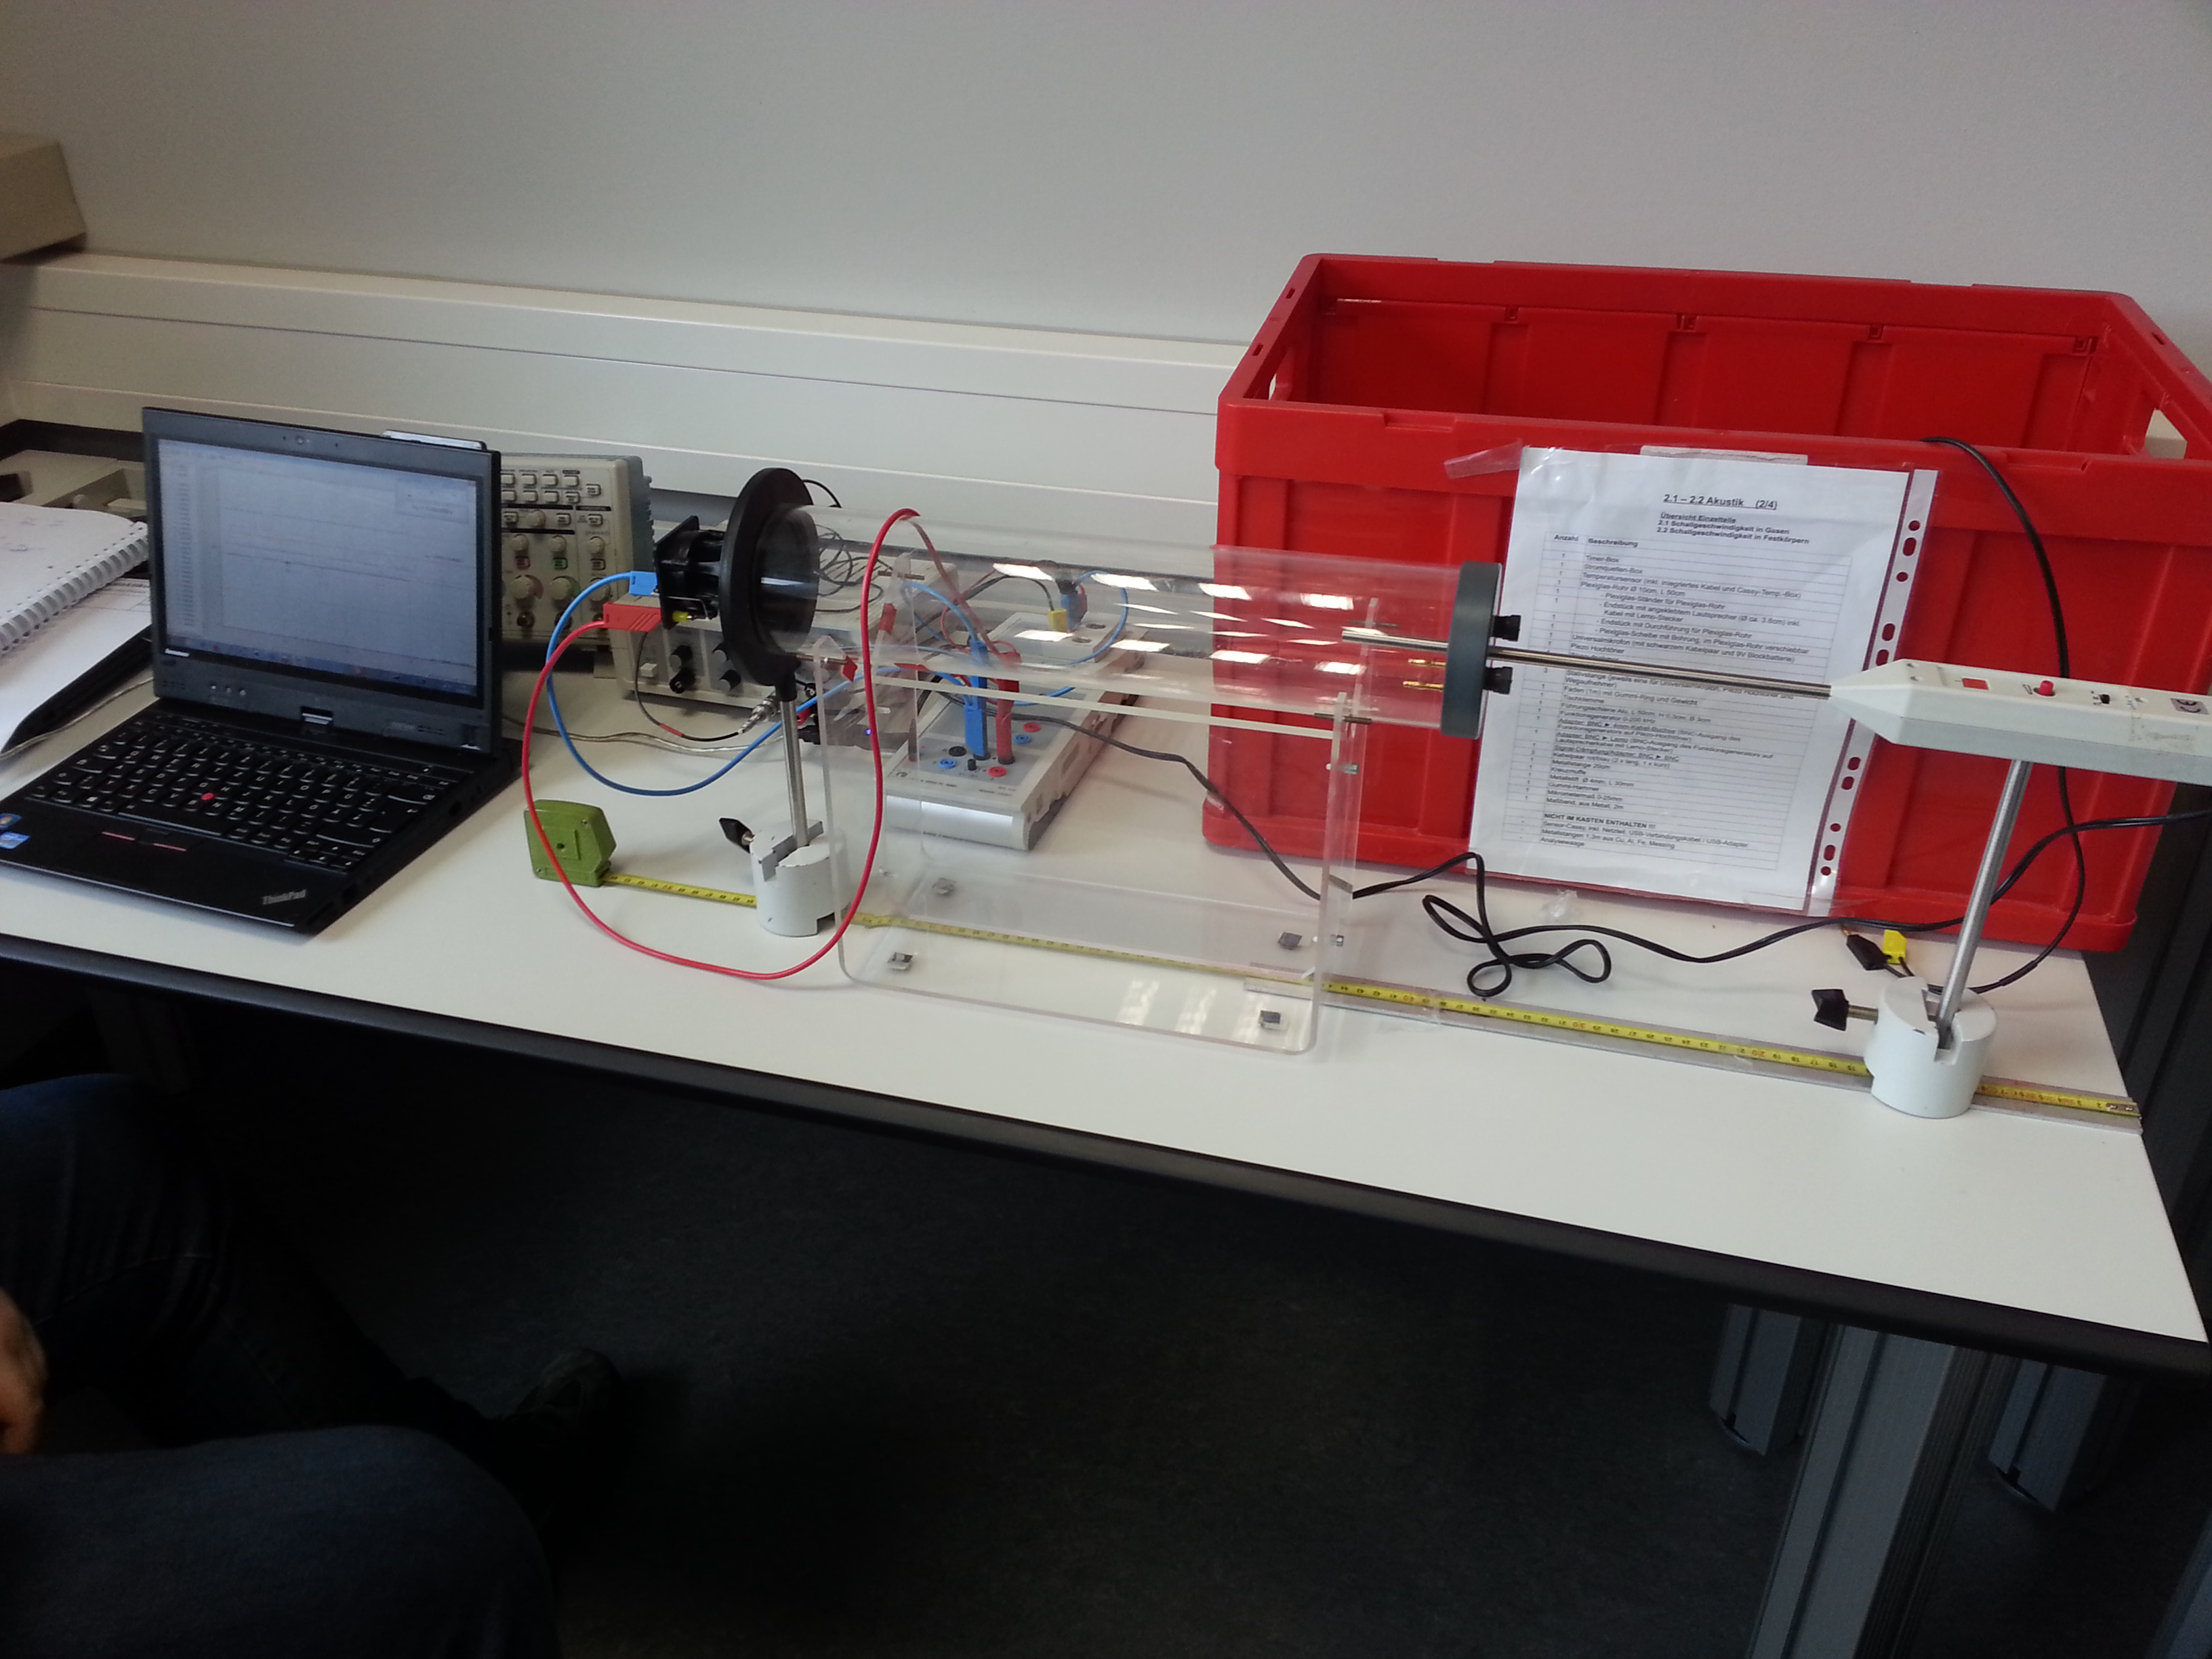
\includegraphics[scale=0.15]{Bilder/laufzeit-cassy.jpg}
\caption{Versuchsaufbau der Laufzeitmessung mit dem Sensor-Cassy.}
\end{figure}



Bei dem Versuch wurde mit einem Piezo-Hochtöner am einen Ende eines Schallrohrs eine Störung erzeugt, die dann in verschiedenen Abständen innerhalb des Schallrohrs von einem Mikrofon im Trigger-Modus aufgezeichnet wurde. Der Piezo-Hochtöner wurde sowohl an eine Timerbox, die an das Sensor-Cassy anschlossen wurde, als auch parallel dazu an das Relais des Sensor-Cassys angeschlossen. Das Mikrofon wurde ebenfalls an die Timerbox angeschlossen. Beim Start der Messung wird das Relais geschlossen, wodurch das Piezoelement entladen wird und die Störung aussendet. Nach Schließen des Relais wird dieses wieder aufgeladen. Beim  Eintreffen der Störung am Mikrofon, liefert dieses das Stopp-Signal für die Zeitmessung.
Anschließend wurde dieser Versuch noch einmal mit einem Oszilloskop aufgezeichnet und der Abstand der Spannungspeaks mit Hilfe des Cursors abgelesen.
Außerdem wurde während des Versuchs die Temperatur der Luft gemessen.
\subsection{Versuchsauswertung}
\subsubsection{Rohdaten}
\begin{figure}[H]
\centering
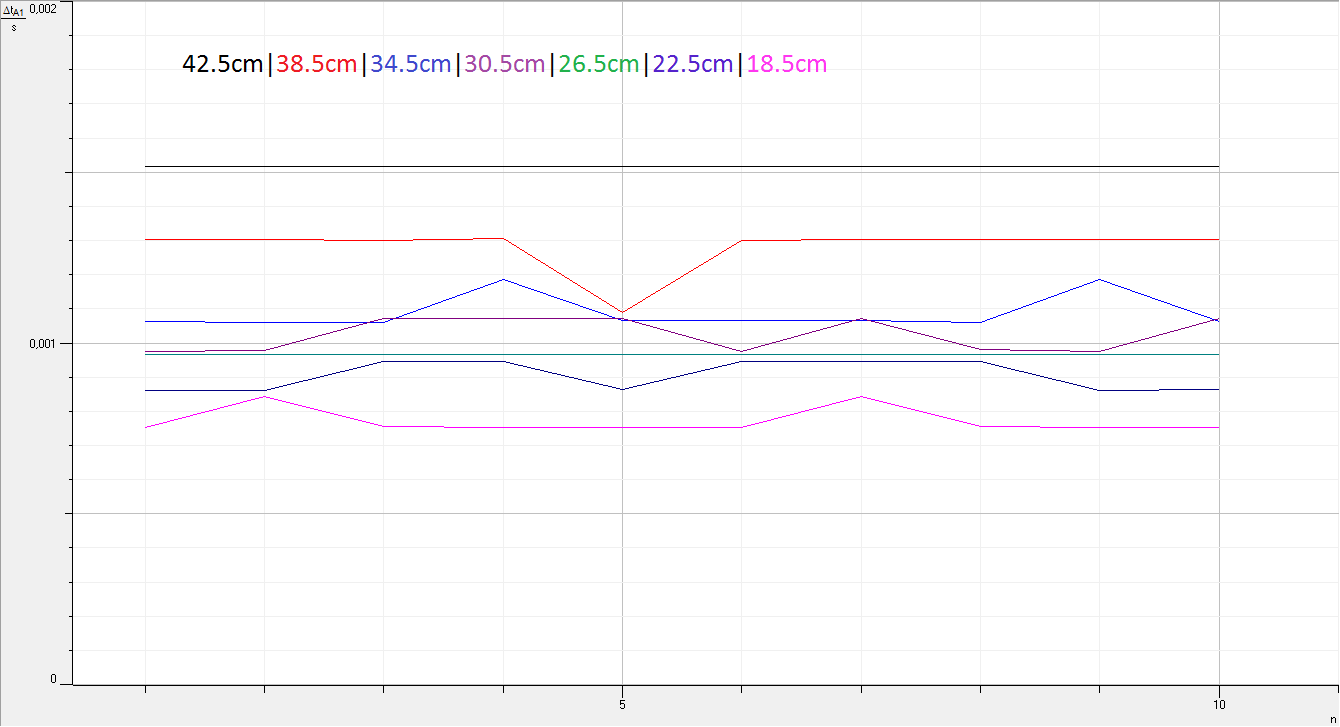
\includegraphics[scale=0.6]{Bilder/Rohdaten-Laufzeitmessung.png}
\caption{Beispiel einer Laufzeitmessung mit dem Sensor-Cassy bei verschiedenen Abständen}
\label{Laufzeitrohdaten}
\end{figure}
\begin{figure}[H]
\centering
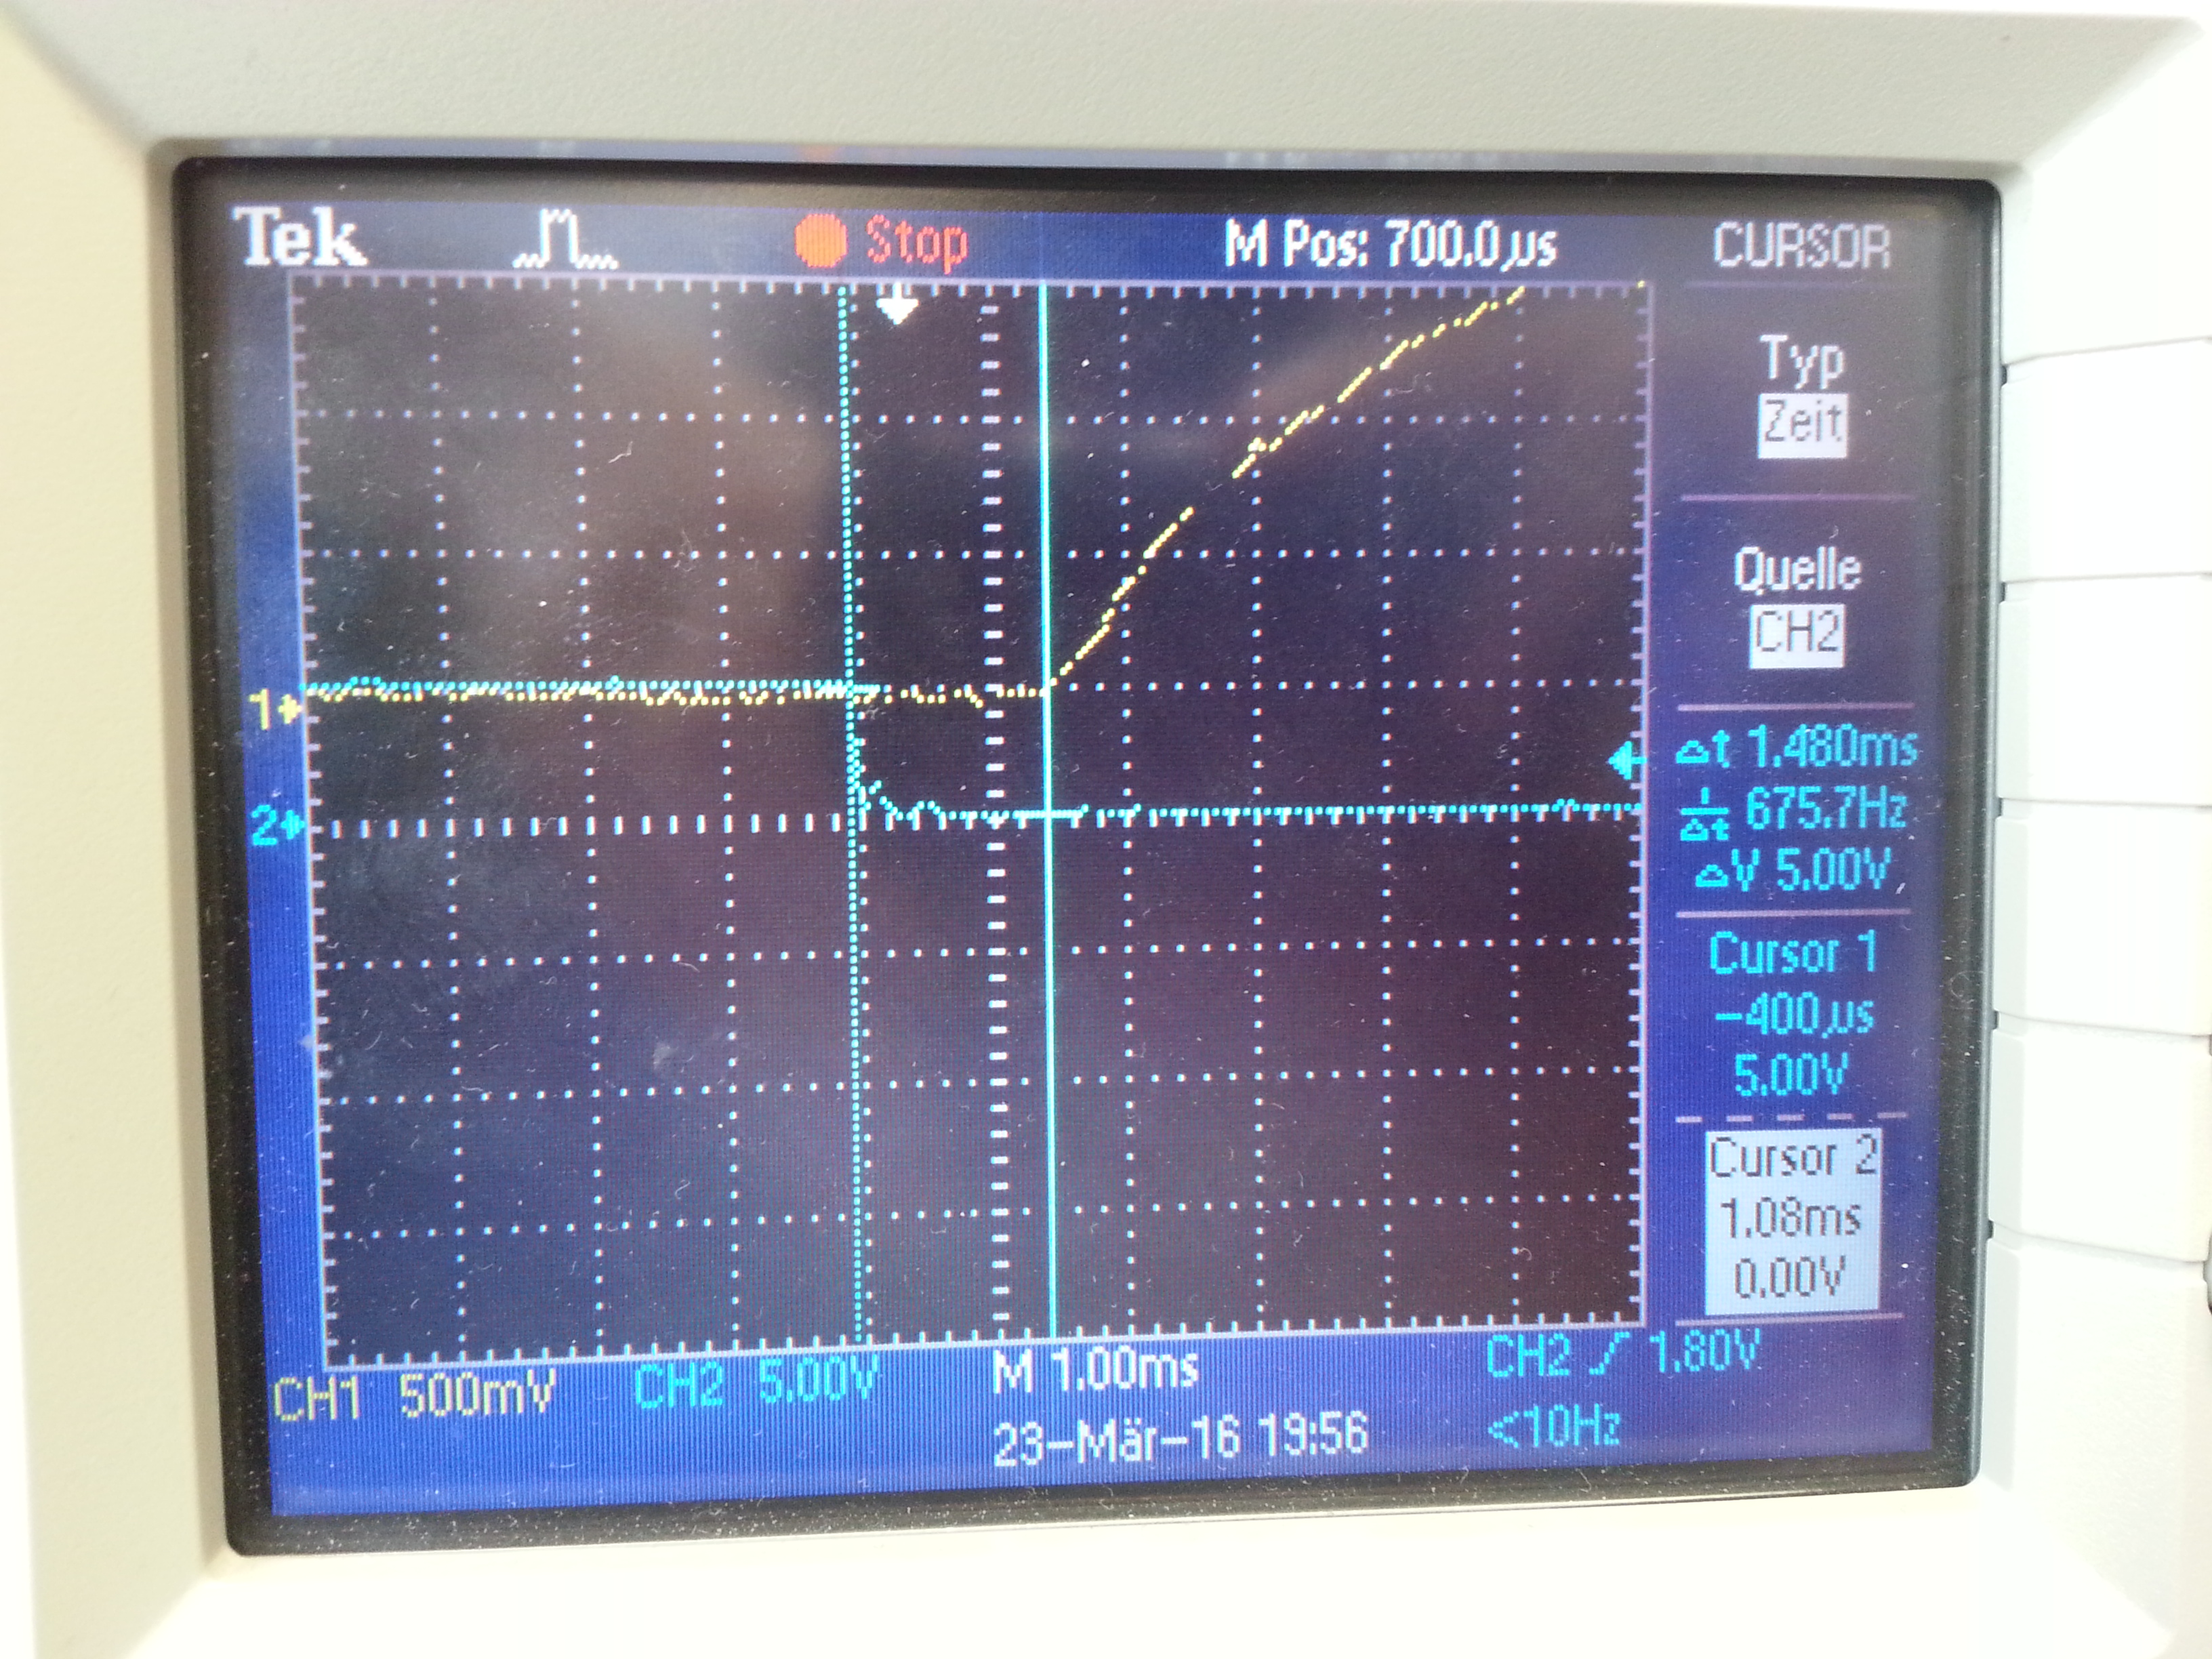
\includegraphics[scale=0.12]{Bilder/oszi.jpg}
\caption{Beispiel einer Laufzeitmessung mit dem Oszilloskop bei einem Abstand von 42.5cm}
\end{figure}
\begin{table}[H]\centering
\caption{Werte der Laufzeitmessung mit dem Oszilloskop}
\begin{tabular}{c|c}
Abstand in m & Zeitdifferenz der Spannungspeaks in ms\\ 
\hline
$42.5$& $1.48$\\ 
$34.5$& $1.24$\\
$26.5$& $1.08$\\
\end{tabular} 
\end{table}
Der Fehler auf die Zeit ergibt sich aus der Auflösung des Oszilloskops zu $0.04ms$.
Die Lufttemperatur betrug während des Versuchs ca. $22.6^{\circ}C$.
\subsubsection{Transformation der Rohdaten/Analyse}
Zur Auswertung wurden die gemessenen Werte der Cassy-Messung für die Zeit bei den jeweiligen Abständen gemittelt und die Fehler bestimmt.
\begin{table}[H]\centering
\caption{Mittelwerte der Cassy-Laufzeitmessung mit Fehlern}
\begin{tabular}{c|c|c}
Abstand in m & Mittelwert der Zeit in ms & $\sigma_t$ in ms\\ 
\hline
$42.5$& $1.51705$& $4.104 \cdot 10^{-4}$\\ 
$38.5$& $1.28692$& $7.141 \cdot 10^{-2}$\\
$34.5$& $1.08284$& $4.526 \cdot 10^{-2}$\\
$30.5$& $1.05089$& $4.390 \cdot 10^{-2}$\\
$26.5$& $0.96639$& $5.193 \cdot 10^{-4}$\\
$22.5$& $0.92490$& $3.756 \cdot 10^{-2}$\\
$18.5$& $0.80627$& $4.416 \cdot 10^{-2}$\\
\end{tabular} 
\end{table}
$~$\newline
Die Mittelwerte mit ihren Fehlern wurde anschließend gegen den Abstand des Mikrofons aufgetragen, eine Lineare Regression durchgeführt und die dazugehörigen Residuen bestimmt.
\newline
Die Auswertung der Daten des Oszilloskops erfolgte analog, nur dass wir keine Werte mitteln mussten.
\begin{figure}[H]
\centering
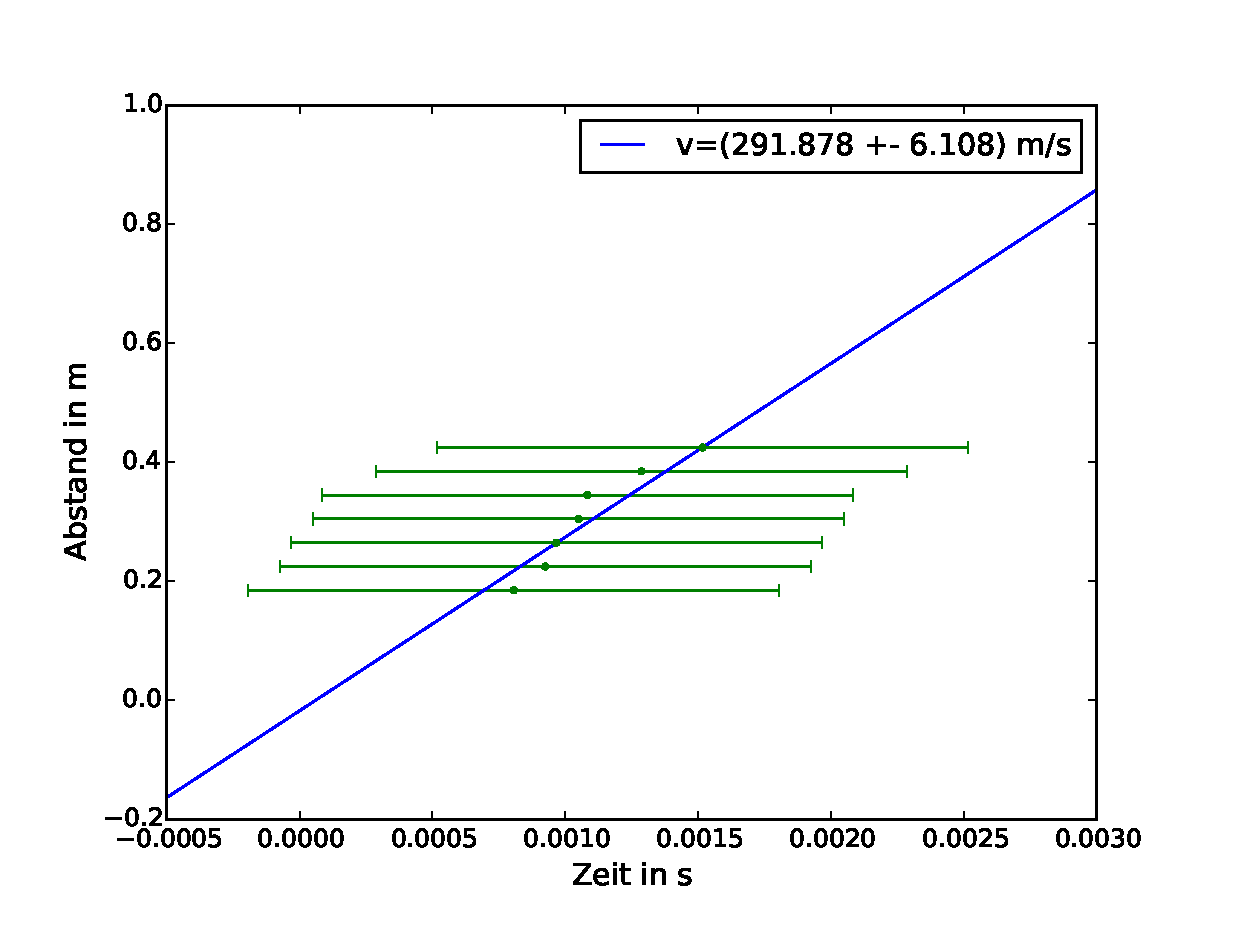
\includegraphics[scale=0.6]{Bilder/Linreg-Laufzeit.eps}
\caption{Lineare Regression durch die Mittelwerte der Cassy-Messung mit ihren Fehlern $\frac{\chi^2}{f}=5.677$}
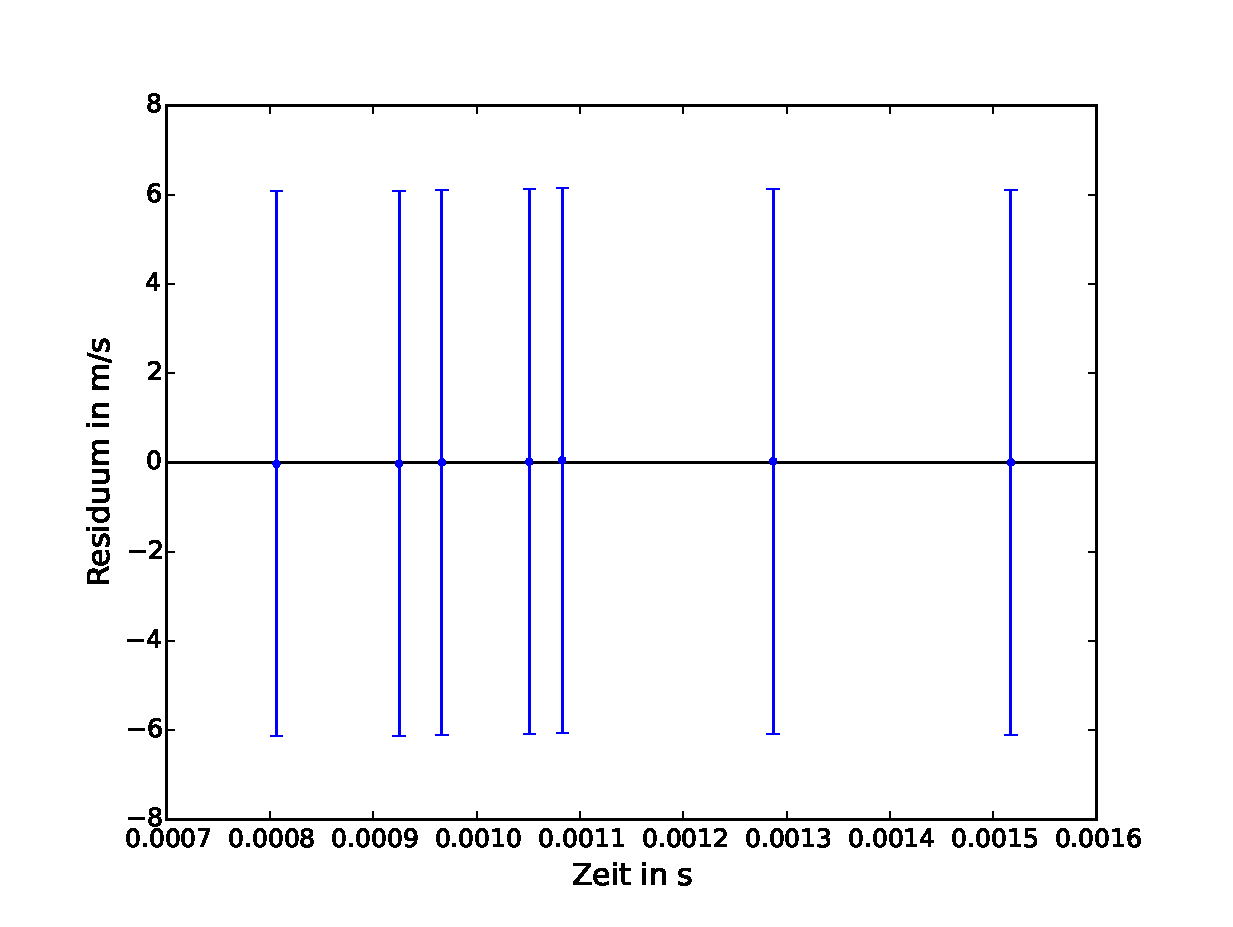
\includegraphics[scale=0.6]{Bilder/Residuen-Laufzeit.eps}
\caption{Residuen des Fits, der Cassy-Messung}
\end{figure}
\begin{figure}[H]
\centering
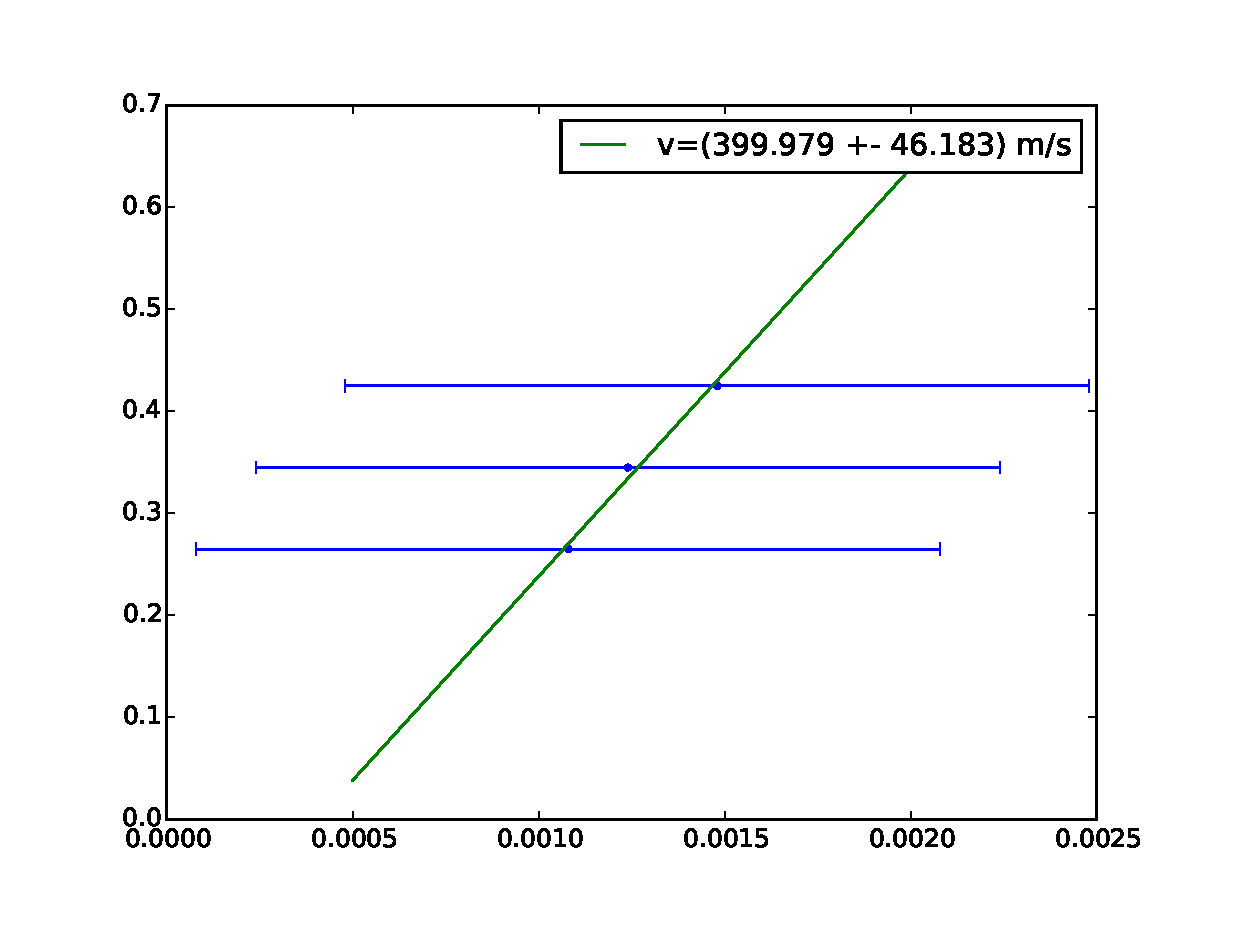
\includegraphics[scale=0.8]{Bilder/Linreg-Oszi.eps}
\caption{Lineare Regression der vom Oszilloskop abgelesenen Werte mit ihren Fehlern $\frac{\chi^2}{f}=0.664$}
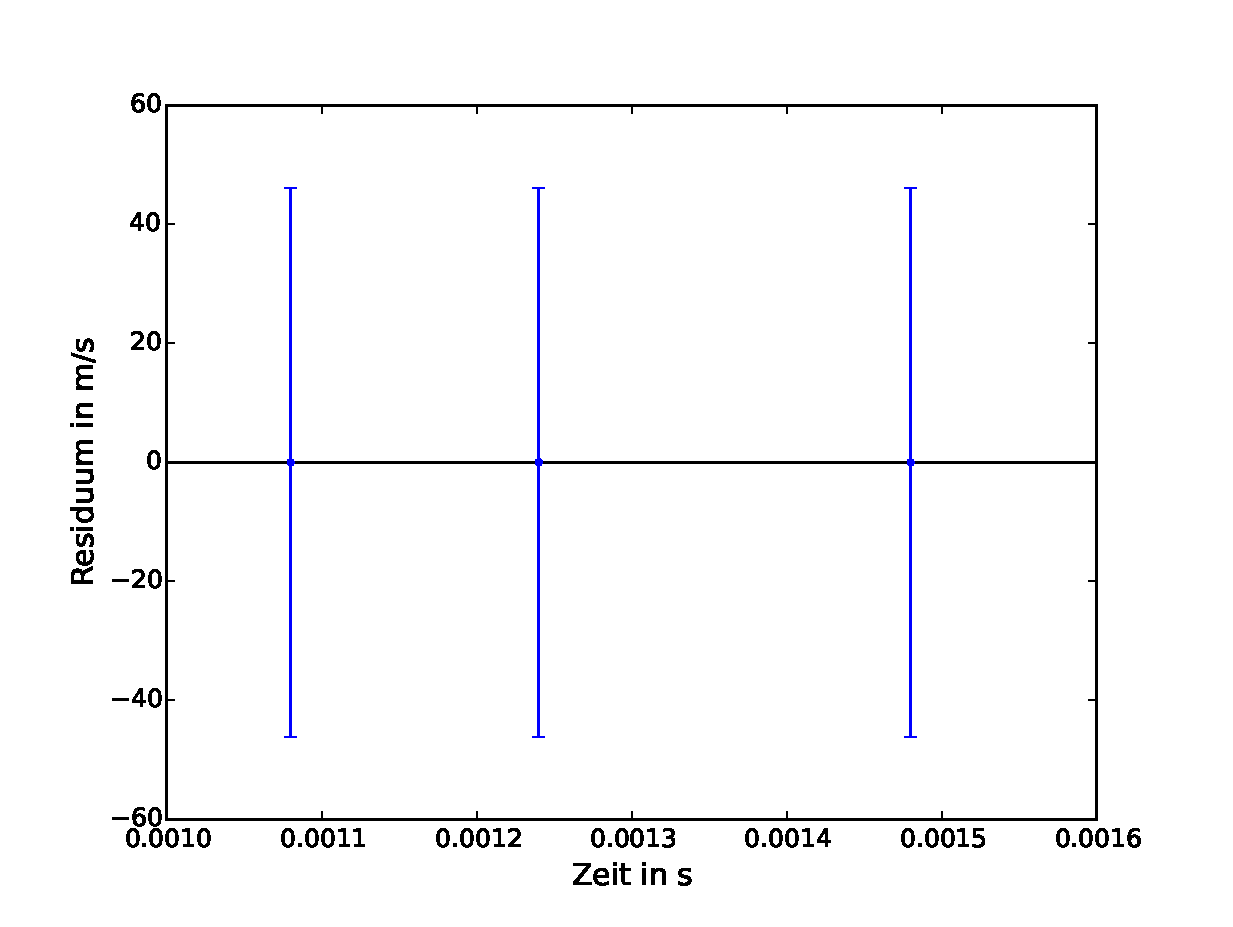
\includegraphics[scale=0.8]{Bilder/Residuen-Oszi.eps}
\caption{Residuen des Fits der Oszilloskop-Messung}
\end{figure}
$~$\newline
Als Ergebnis für die Schallgeschwindigkeit in Luft erhalten wir also einen Wert von \newline $v=(291.878 \pm 6.108) \frac{m}{s}$ für die Cassy-Messung und einen Wert von\newline $v=(399.979 \pm 46.183)\frac{m}{s}$.
\subsubsection{Fazit}
Der Literaturwert der Schallgeschwindigkeit in Luft beträgt bei einer Temperatur von $20^{\circ}C$, $342.46\, \frac{m}{s}$. Mit Gleichung (\ref{Temperaturabhängigkeit}) ergibt sich damit ein Wert von $344.98 \, \frac{m}{s}$.
Unser Ergebnis von $v=(291.878 \pm 6.108) \frac{m}{s}$ bei der Cassy-Messung weicht damit um $8\sigma$ vom Literaturwert ab. Dies erklären wir uns durch starke Streuung unserer Messwerte, bei ein und der selben Distanz (siehe Abbildung (\ref{Laufzeitrohdaten})). \newline
Unser Ergebnis von $v=(399.979 \pm 46.183)\frac{m}{s}$ bei der Oszilloskop-Messung weicht um etwas mehr als $1\sigma$ vom Literaturwert ab und ist somit völlig zufriedenstellend.
\section{Bestimmung der Schallgeschwindigkeit durch Vermessen einer stehenden Welle}
\subsection{Versuchsbeschreibung}
In diesem Versuch werden wir den Wert der Schallgeschwindigkeit über das Vermessen einer stehenden Welle bestimmen. Der Zusammenhang zwischen der Position der Bäuche der stehenden Welle, der angeregten Resonanzfrequenz und der Schallgeschwindigkeit wird durch folgende Formel beschrieben:
\begin{equation}
v_{Schall} = \lambda\cdot f
\end{equation}
Wir werden den Schalldruck an verschiedenen Stellen innerhalb des Rohres bei einer stehenden Welle messen. Danach tragen wie die Amplitude des Schalldrucks gegen die Strecke auf und suchen die Extrema. Diese Punkte werden dann in einer Linearen Regression verwendet. Die Steigung gibt uns $\frac{\lambda}{2}$ zurück, daraus können wir dann zusammen mit der bereits eingestellten Frequenz die Schallgeschwindigkeit berechnen.

\subsection{Versuchsaufbau und Durchführung}
Verwendete Geräte:
\begin{itemize}
\item Frequenzgenerator
\item Sensor-Cassy
\item Richtmikrofon
\item Lautsprecher
\item Rohr ($0.425\, m \pm 0.001\,$m (Messfehler auf Massband))
\item Massband ($\sigma_{Massband} = 0.001\, m$)
\end{itemize}
Wir haben unser Cassy mit folgenden Einstellungen verwendet:
\begin{itemize}
\item Kanal A / Spannung UA1 / $-10..10\, V$ /
\item Kanal B / Timerbox / Frequenz fb1(E) / $5000\, Hz$ / Torzeit: $1\, s$
\item manuelle Messung
\item Darstellung: X-Achse n / Y-Achse Ua1
\end{itemize}
Den Frequenzgenerator haben wir wie folgt eingestellt:
\begin{itemize}
\item Signalform / $\sim$ (Sinusschwingung)
\item Bereich / $x1k (0.2 - 2.4 x 1\, $kHz$)$
\item $\sigma_f = 10\,$Hz (Abschätzung durch ungenaue Feinabstimmung, gerätbedingt)
\item Offset / 0
\item Amplitude / mittig
\end{itemize}
Die Raumtemperatur betrug $23^{\circ}\, C$.
\begin{figure}[H]
\centering
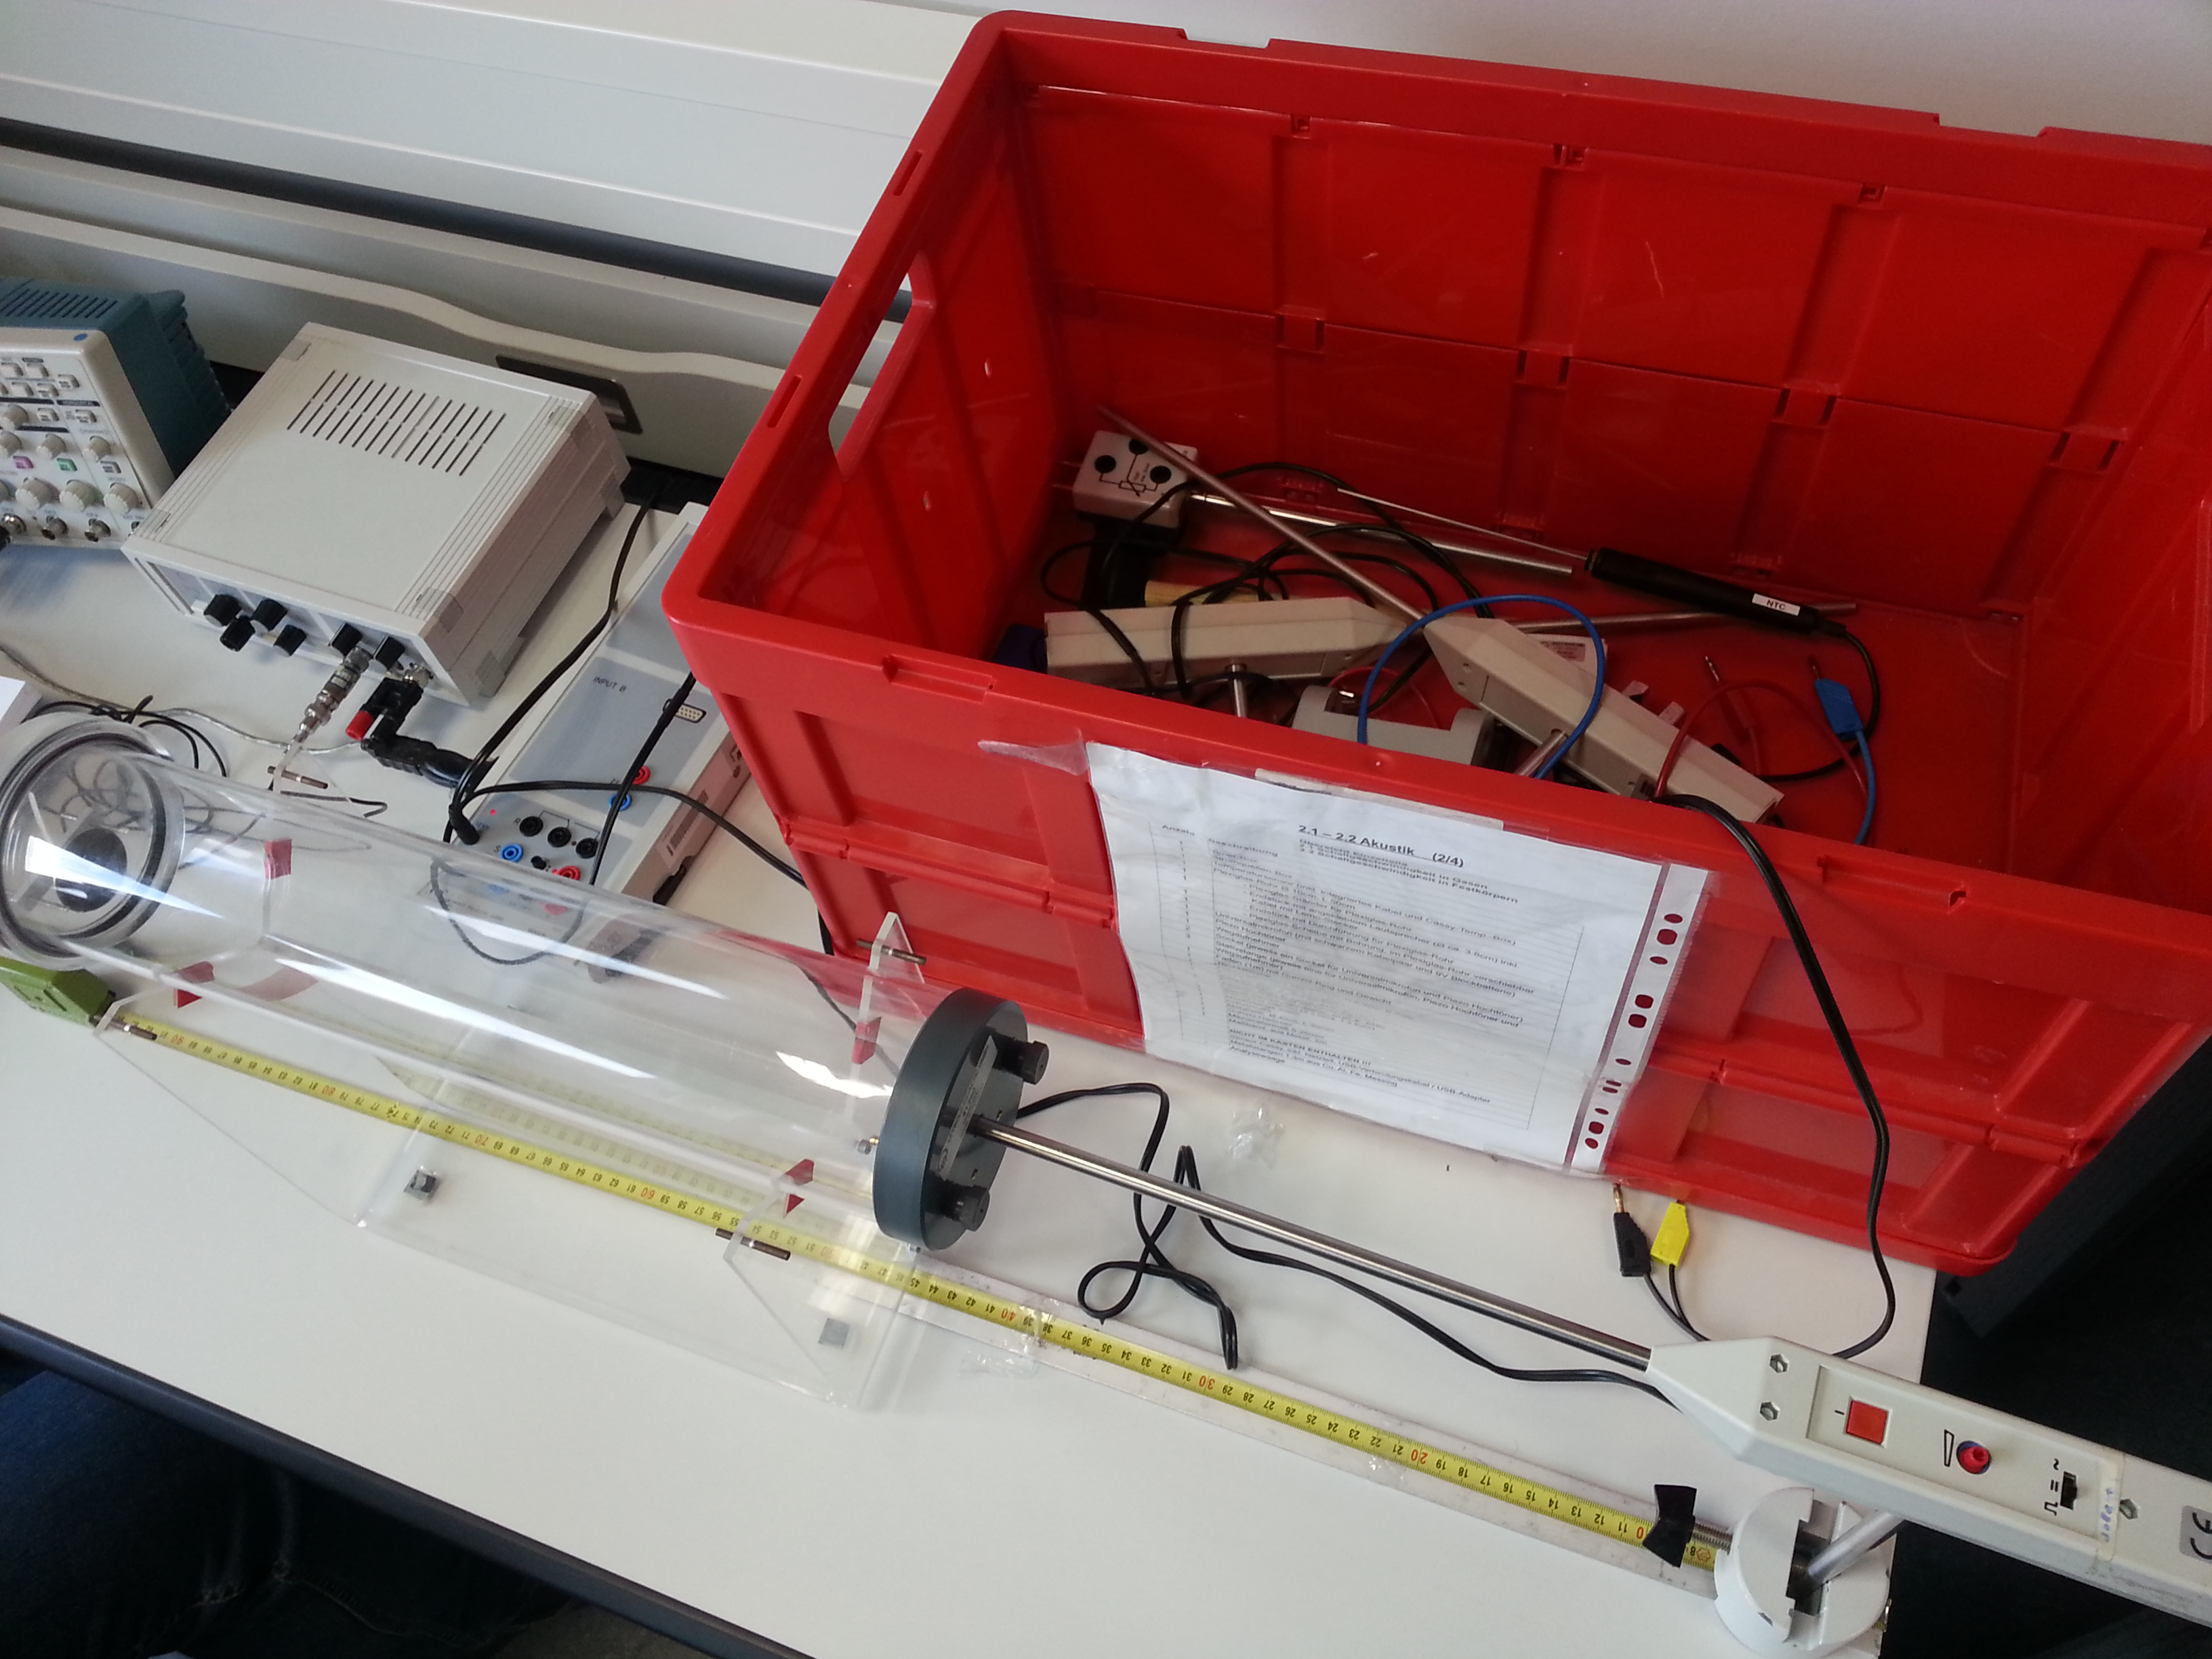
\includegraphics[scale=0.1]{Bilder/Druckknoten-Messung3.jpg}
\caption{Versuchsaufbau für die Bestimmung der Schallgeschwindigkeit über die Vermessung einer stehenden Welle}
\end{figure}
Durchführung:\newline
Wir messen alle 0.5$\,$cm angefangen bei 2.5$\,$cm (gemessen vom Anfang der Schiene). Die Umrechnung von n in m lautet also wie folgt:
\begin{equation}
l = (0.025 + n\cdot 0.005) - 0.425
\end{equation}
wobei die 42.5$\,$cm die Länge des Rohres beschreibt, wie unter Geräte angegeben.
Die sich so ergebenen Daten sehen wie folgt aus:
\begin{figure}[H]
\centering
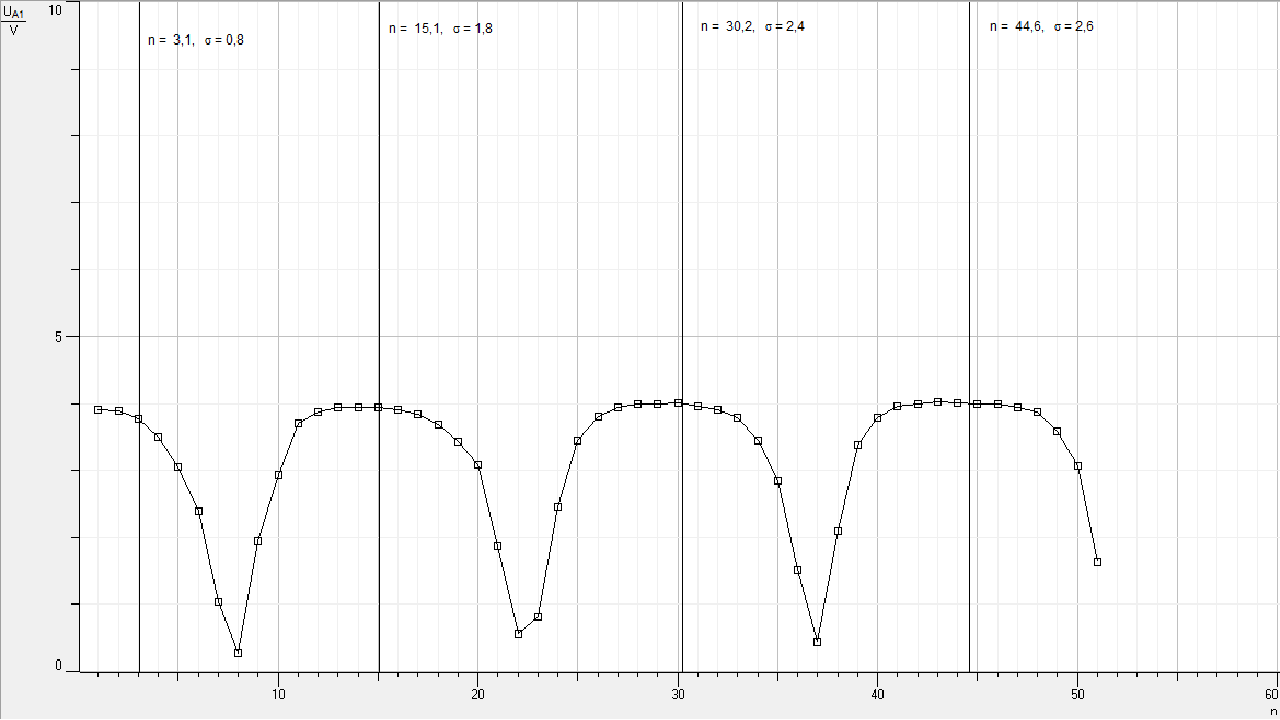
\includegraphics[scale=0.3]{Bilder/baeuche.png}
\caption{Amplitude des Schalldrucks aufgetragen gegen eingeführte Länge des Richtmikrofons (in n - Umrechnung siehe oben)}
\end{figure}
Wir haben leider wenig Punkte bei den Knoten, daher werden wir für unsere Lineare Regression nur unsere Peaks betrachten. Diese bestimmen wir mit der Peaksschwerpunktfunktion von Cassy.
Die sich daraus ergebenen Daten sind unter Rohdaten aufgeführt.

\subsection{Versuchsauswertung}

\subsubsection{Rohdaten}
\begin{table}[H]
\begin{tabular}{c|c|c}
Position Bauch N & Messpunkt n & Länge [m] \\ 
\hline 
1.5 & 1 & 0.395 \\ 
2.5 & 15 & 0.325 \\ 
3.5 & 30 & 0.25 \\ 
4.5 & 45 & 0.175 \\ 
\end{tabular}
\caption{Druckbäuche für $f = 2400\,$Hz, mit $\sigma_l = 0.0028\,$m}
\end{table}
\subsubsection{Transformation der Rohdaten}
Mit den oben genannten Rohdaten führen wir jetzt eine Lineare Regression durch. Die Steigung der Linearen Regression gibt uns $\frac{\lambda}{2}$ zurück und beträgt $0.0735\,$m. Unsere Lineare Regression sieht wie folgt aus:
\begin{figure}[H]
\centering
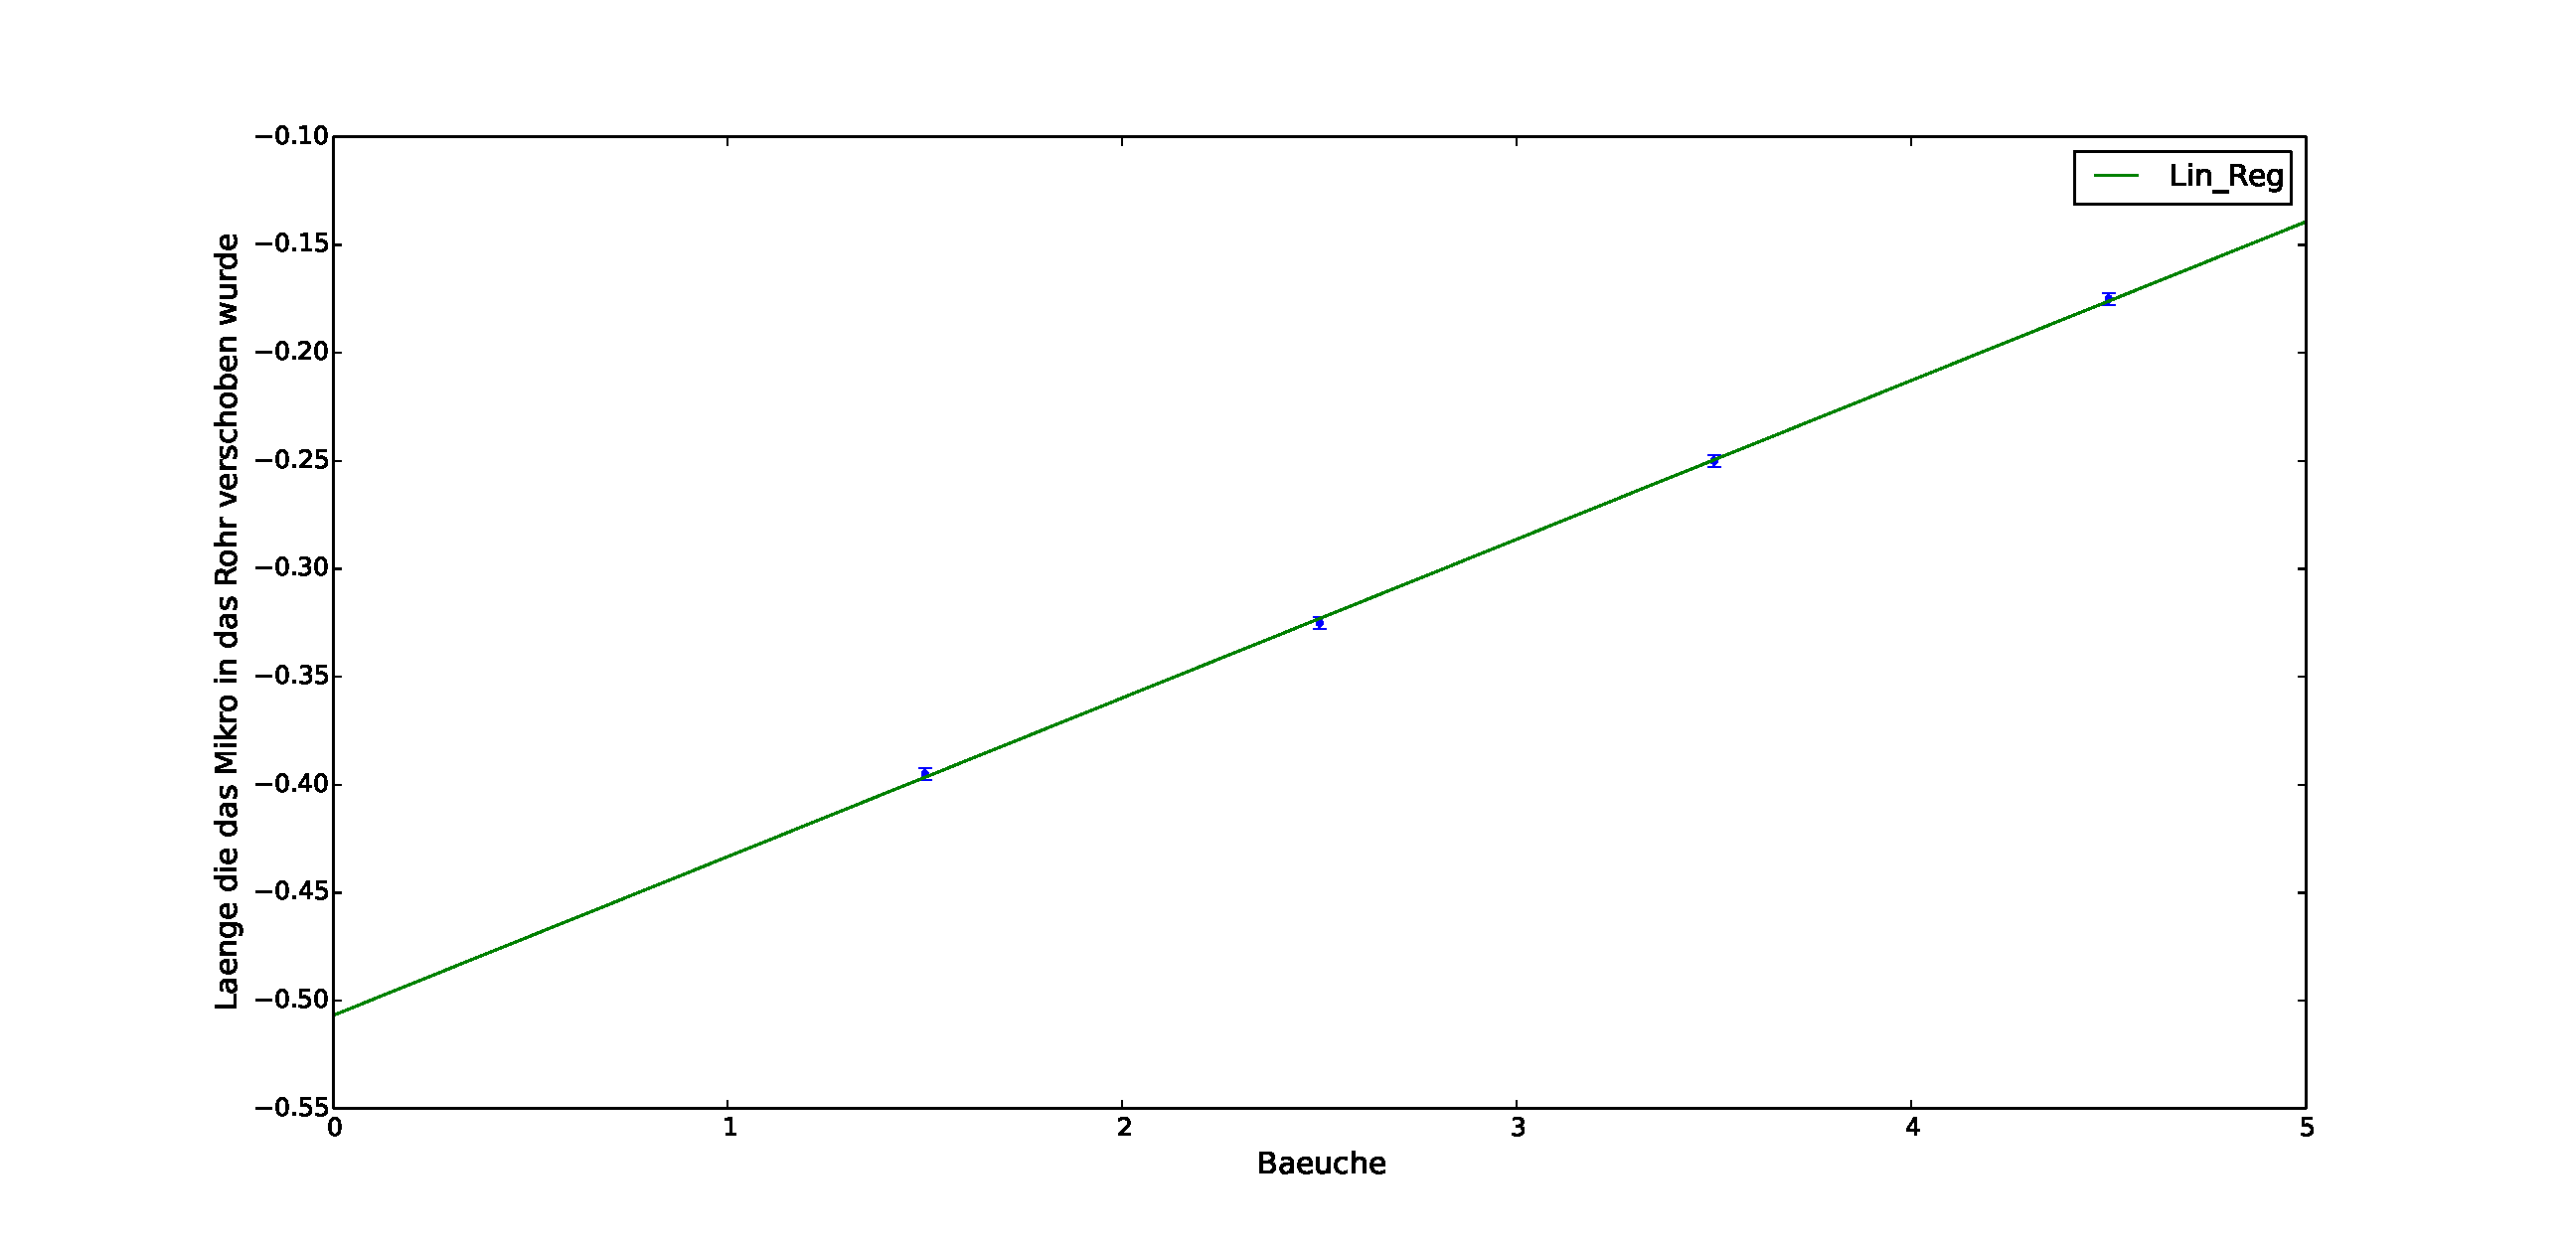
\includegraphics[scale=0.3]{Bilder/linreg_stehende_welle.eps}
\caption{Lineare Regression der 4 oben genannten Peaks, die Steigung beträgt $\frac{\lambda}{2}$}
\end{figure}
Wir haben dabei ein $\chi^2 = 0.47$ erreicht.
Unser Residuenplot dazu sieht wie folgt aus:
\begin{figure}[H]
\centering
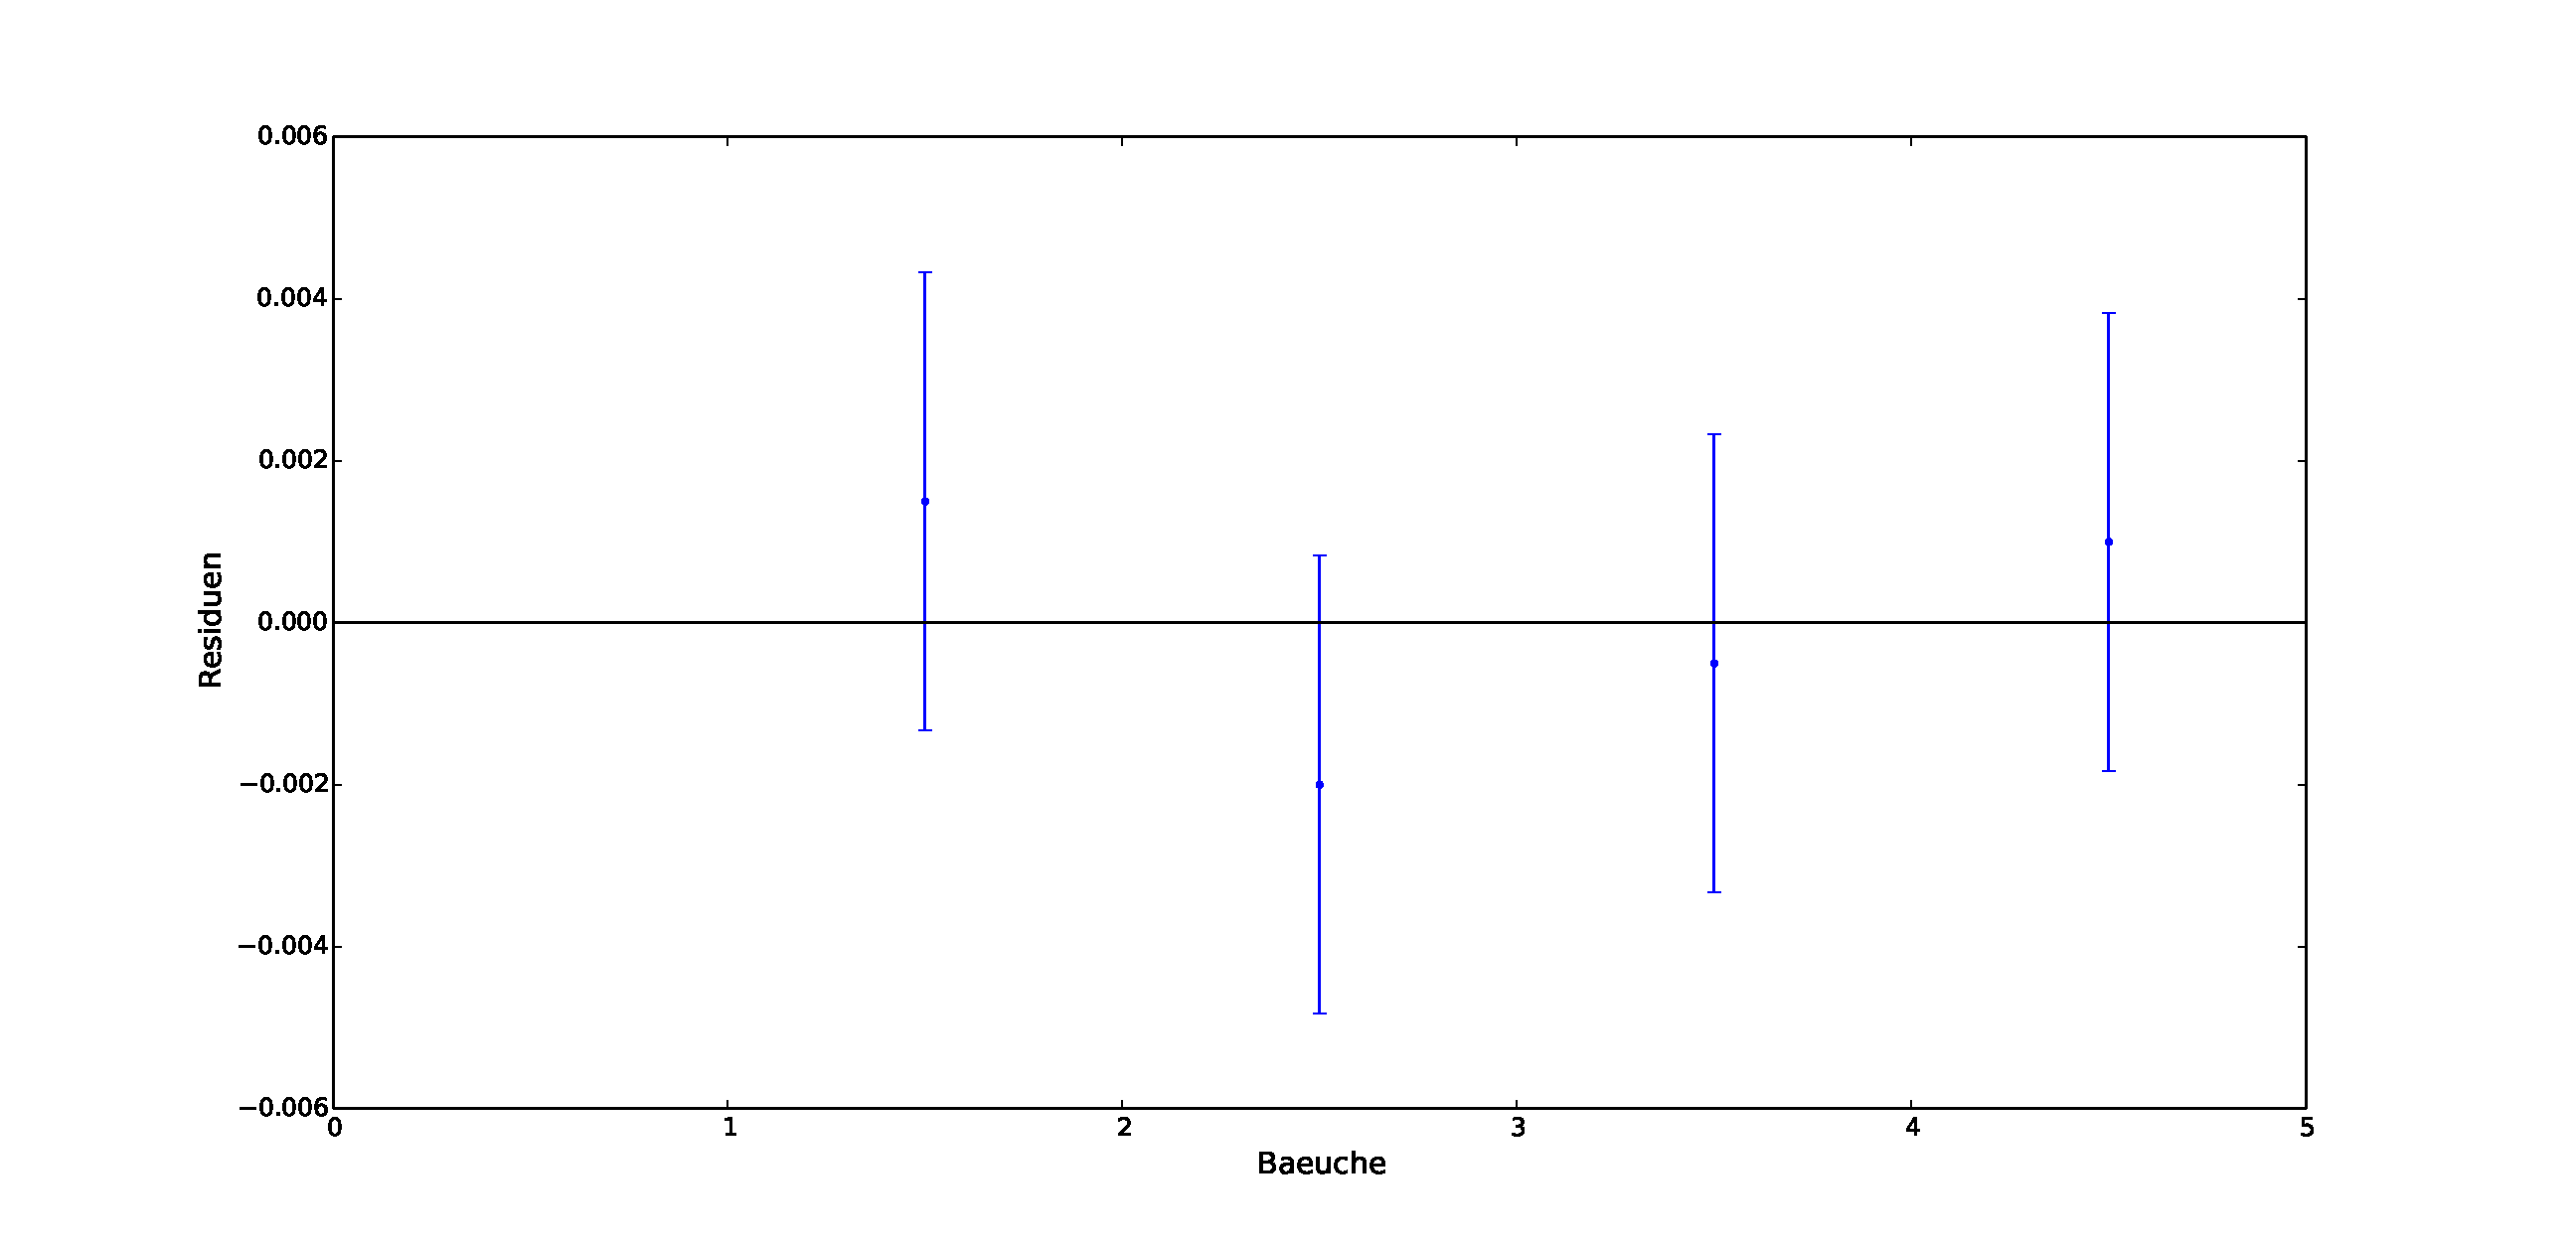
\includegraphics[scale=0.3]{Bilder/residuen_stehende_welle.eps}
\caption{Residuenplot (Daten - Fit) mit den jeweiligen Fehlern}
\end{figure}
Alle Werte liegen mit ihren Fehlern in einem Abstand kleiner als $\sigma$ von 0 entfernt. Die Werte sind gleichverteilt um 0 gestreut und es lässt sich keine Systematik erkennen.\newline
Um auf unseren Wert für $v$ zu kommen müssen wir die eingestellte Frequenz $f = 2400\,$Hz und die mit dem Faktor 2 multiplizierte Steigung (wir erinnern uns, dass die Steigung der Linearen Regression nur $\frac{\lambda}{2}$ zurückgab) der Linearen Regression in die am Anfang dieses Kapitels eingeführte Gleichung
\begin{equation*}
v = \lambda\cdot f
\end{equation*}
einsetzen. So erhalten wir einen Wert für $v = 352.8\,\frac{m}{s}$.
Um den Fehler auf $v$ zu erhalten, müssen wir $\sigma_{\lambda}$ und $\sigma_f$ fortpflanzen.
\begin{equation}
\sigma_{v} = \sqrt{f^2\cdot\sigma_{\lambda}^2 + \lambda^2\cdot\sigma_{f}^2}
\end{equation}
mit $\sigma_{\lambda} = 0.0025\,$m (aus Ausgabe der Linearen Regression.)
Daraus ergibt sich für unser Ergebnis, dass die Schallgeschwindigkeit $v_{Schall} = 352.8 \pm 4.5\,\frac{m}{s}$ beträgt.

\subsection{Fazit}
Unser Ergebnis für die Schallgeschwindigkeit liegt innerhalb von 2$\sigma_{v}$ über dem Literaturwert (bei T$ = 20^{\circ}\,$C beträgt die Schallgeschwindigkeit $v = 343.\,\frac{m}{s}$, umgerechnet für T$ = 22.6^{\circ}\,$C mit $v = v_0\cdot\sqrt{\frac{T}{T_0}}$, $v = 344.98\,\frac{m}{s}$). Wir erklären uns diese Abweichung durch die fehlenden Werte für die Druckknoten der stehenden Welle in der Linearen Regression. Ansonsten sind wir sowohl mit unserer Anpassung ($\chi^2 = 0.47$) als auch mit der um 0 gleichverteilt gestreuten Residuen zufrieden.
\section{Vermessung der Schallgeschwindigkeit durch Variation der Frequenz}
\subsection{Versuchsberschreibung}
In diesem Versuch werden wir die Schallgeschwindigkeit aus der Steigung der Geraden 
\begin{equation}
f_n = \frac{n\cdot v}{2\cdot L}
\end{equation}
bestimmen. Dabei steht $f_n$ für die Resonanzfrequenzen, n für die Vielfache, v für die Schallgeschwindigkeit und L für die Länge des Rohres. Dafür vermessen wir zunächst grob die Resonanzfrequenzen.
Danach werden wir das gleiche noch einmal genau wiederholen, aber mit deutlich mehr Messpunkten um die jeweiligen Resonanzfrequenzen (siehe Bild), insgesamt 3 mal.

\subsection{Versuchsaufbau und Durchführung}
Verwendete Geräte:
\begin{itemize}
\item Frequenzgenerator
\item Sensor-Cassy
\item Richtmikrofon
\item Lautsprecher
\item Rohr ($0.425\, m \pm 0.001\,$ m (Messfehler auf Massband))
\item Massband ($\sigma_{Massband} = 0.001\, m$)
\end{itemize}
Wir haben unser Cassy mit folgenden Einstellungen verwendet:
\begin{itemize}
\item Kanal A / Spannung UA1 / $-10..10\, V$ /
\item Kanal B / Timerbox / Frequenz fb1(E) / $5000\, Hz$ / Torzeit: $1\, s$
\item manuelle Messung
\item Darstellung: X-Achse fb1 / Y-Achse Ua1
\end{itemize}
Den Frequenzgenerator haben wir wie folgt eingestellt:
\begin{itemize}
\item Signalform / $\sim$ (Sinusschwingung)
\item Bereich / $x1k (0.2 - 2.4 x 1\, $kHz$)$
\item $\sigma_f = 10\,$Hz (Abschätzung durch ungenaue Feinabstimmung, gerätbedingt)
\item Offset / 0
\item Amplitude / mittig
\end{itemize}
\begin{figure}[H]
\centering
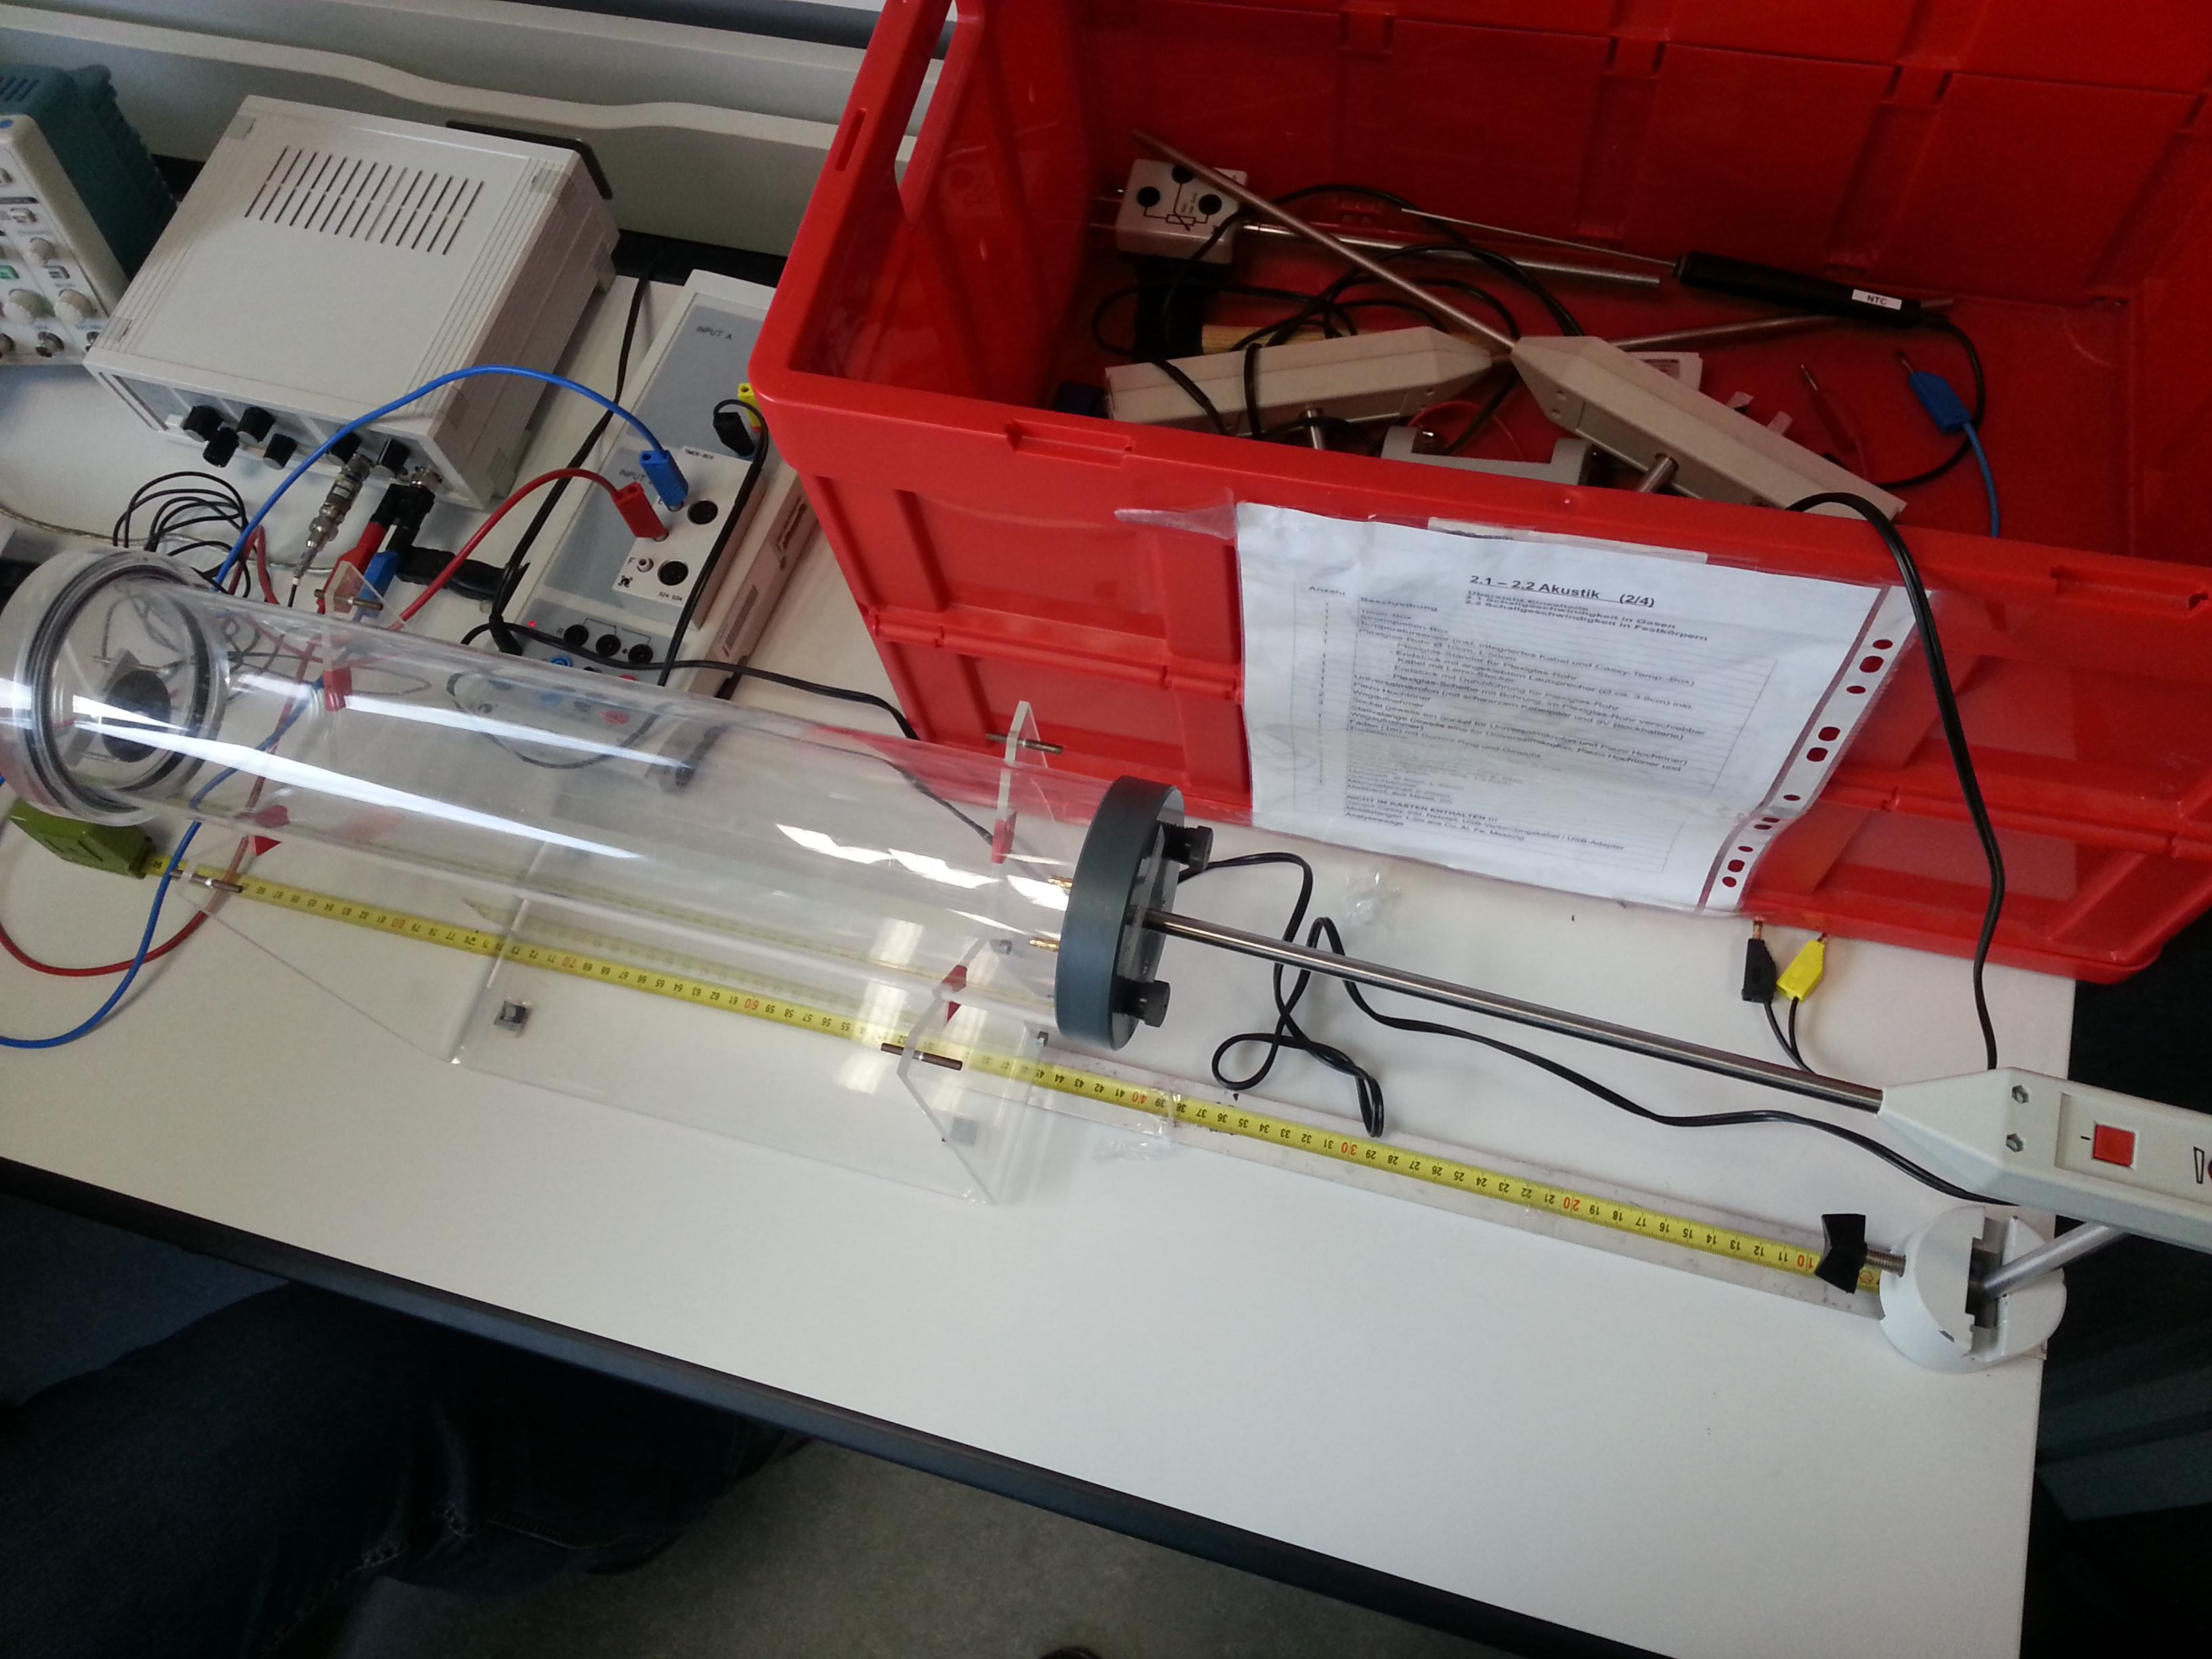
\includegraphics[scale=0.15]{Bilder/Frequenzvariation3.jpg}
\caption{Versuchsaufbau zur Messung der Schallgeschwindigkeit durch Variation der Resonanzfrequenzen}
\end{figure}
Zunächst haben wir grob die Resonanzfrequenz bestimmt:
\begin{figure}[H]
\centering
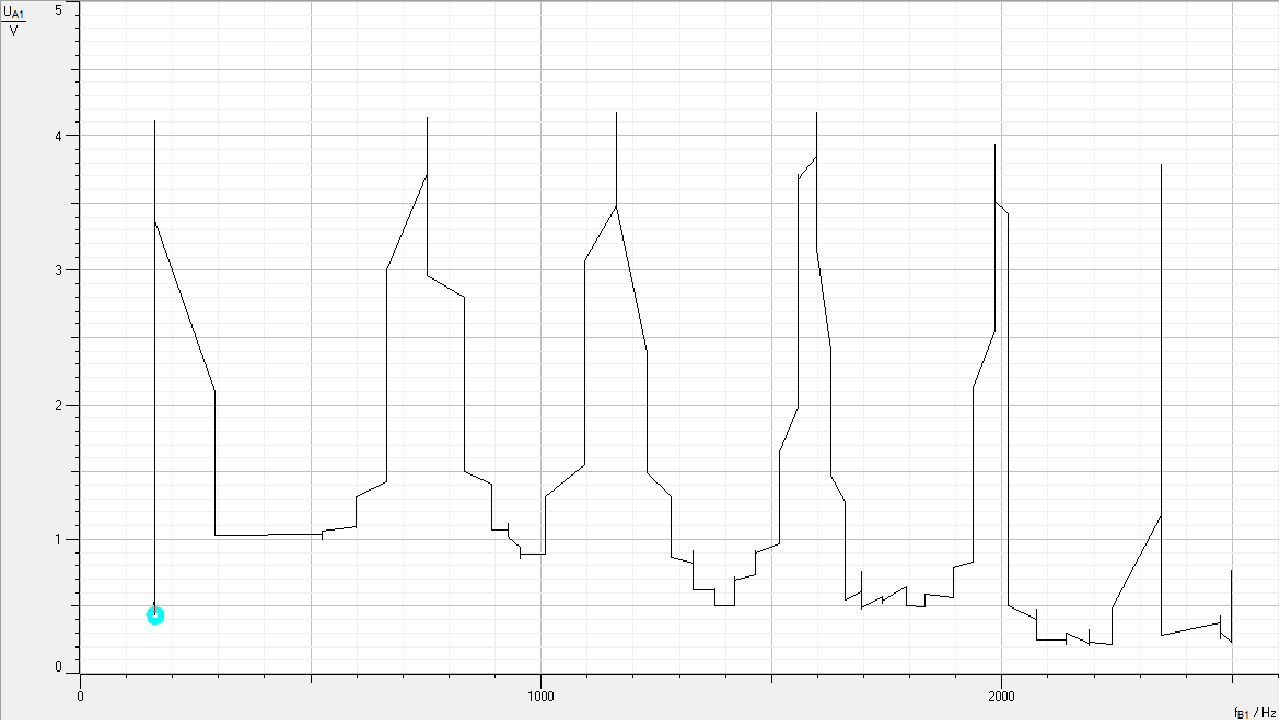
\includegraphics[scale=0.5]{Bilder/grobevermessung.png}
\caption{Grobe Vermessung der Resonanzfrequenzen - die deutlich ausgeprägten Peaks werden später genauer untersucht.}
\end{figure}
Danach haben wir an den oben zu sehenden Peaks das ganze noch mal mit mehr Messpunkten in drei Messungen gemessen:
\begin{figure}[H]
\centering
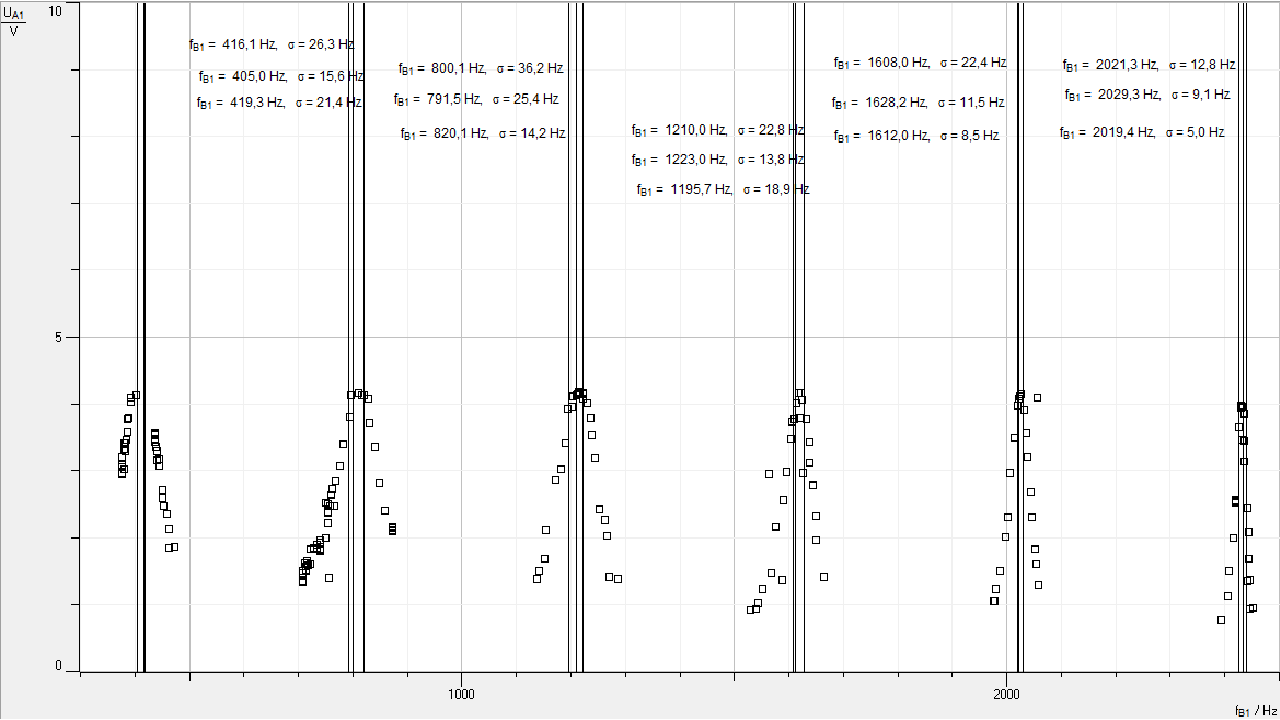
\includegraphics[scale=0.5]{Bilder/vermessung_variation_genau.png}
\caption{genaue Vermessung der Peaks an einer Beispiel Messung}
\end{figure}
Die sich daraus ergebenen Daten sind unter Rohdaten aufgeführt.
\subsection{Versuchsauswertung}
\subsubsection{Rohdaten}
\begin{table}[H]
\begin{tabular}{c|c|c|c|c|c|c}
vermutete Resonanzfrequenz & 400 & 800 & 1200 & 1600 & 2000 & 2400 \\ 
\hline 
Peak Messung I & 416.0 & 822.5 & 1210.0 & 1608.0 & 2031.1 & 2433.4 \\  
$asym_r$ Peak Messung I & 417.0 & 826.8 & 1212.6 & 1629.6 & 2041.4 & 2443.7 \\  
$asym_l$ Peak Messung I & 404.9 & 798.2 & 1190.0 & 1573.9 & 2019.3 & 2425.5 \\ 
\hline 
Peak Messung II & 420.7 & 822.1 & 1210.9 & 1620.0 & 2037.2 & 2446.7 \\  
$asym_r$ Peak Messung II & 423.0 & 836.4 & 1216.5 & 1631.3 & 2047.8 & 2467.3 \\ 
$asym_l$ Peak Messung II & 404.3 & 797.5 & 1194.0 & 1612.3 & 2013.8 & 2421.3 \\ 
\hline 
Peak Messung III & 416.1 & 800.1 & 1210.0 & 1612.0 & 2019.4 & 2433.4 \\  
$asym_r$ Peak Messung III & 419.3 & 820.1 & 1223.0 & 1628.2 & 2029.3 & 2439.2 \\  
$asym_l$ Peak Messung III & 405.0 & 791.5 & 1195.7 & 1608.0 & 2019.4 & 2425.5
\end{tabular}
\caption{Vermessung der Resonanzfrequenzen, wobei $asym_r$ und $asym_l$ die asymmetrische Peakvermessung in Cassy (alle Angaben in Hz)} 
\end{table}
Die Raumtemperatur betrug $23^{\circ}\, C$.
\subsubsection{Transformation der Rohdaten}
\begin{table}[H]
\begin{tabular}{c|c|c|c|c|c|c}
vermutete Resonanzfrequenz & 400 & 800 & 1200 & 1600 & 2000 & 2400 \\ 
\hline 
$\bar{M}$ & 412.92 & 812.80 & 1206.97 & 1614.70 & 2030.07 & 2437.33 \\ 
\hline 
$\sigma_{\bar{M}}$ & 6.94 & 16.00 & 11.16 & 18.21 & 10.90 & 14.32 \\ 
\end{tabular}
\caption{Mittelwerte und deren Fehler (alle Angaben in Hz)} 
\end{table}
Nachdem wir die Mittelwerte auf die einzelnen Resonanzfrequenzen und den Fehler auf den Mittelwert  berechnet haben werden wir diese Daten für eine Lineare Regression verwenden. Wir fitten eine Funktion der Form $Fit = m\cdot x + b$.
\begin{equation}
\bar{M} = \frac{\sum_{i=1}{n}{X_i}}{n}
\end{equation}
und
\begin{equation}
\sigma_{\bar{M}} = \frac{\sqrt{\frac{\sum_{i=1}^{N}({X_i-\bar{M}})^2}{N-1}}}{\sqrt{N}}
\end{equation} 
Dabei tragen wir unsere Resonanzen gegen die Mittelwerte auf.
\begin{figure}[H]
\centering
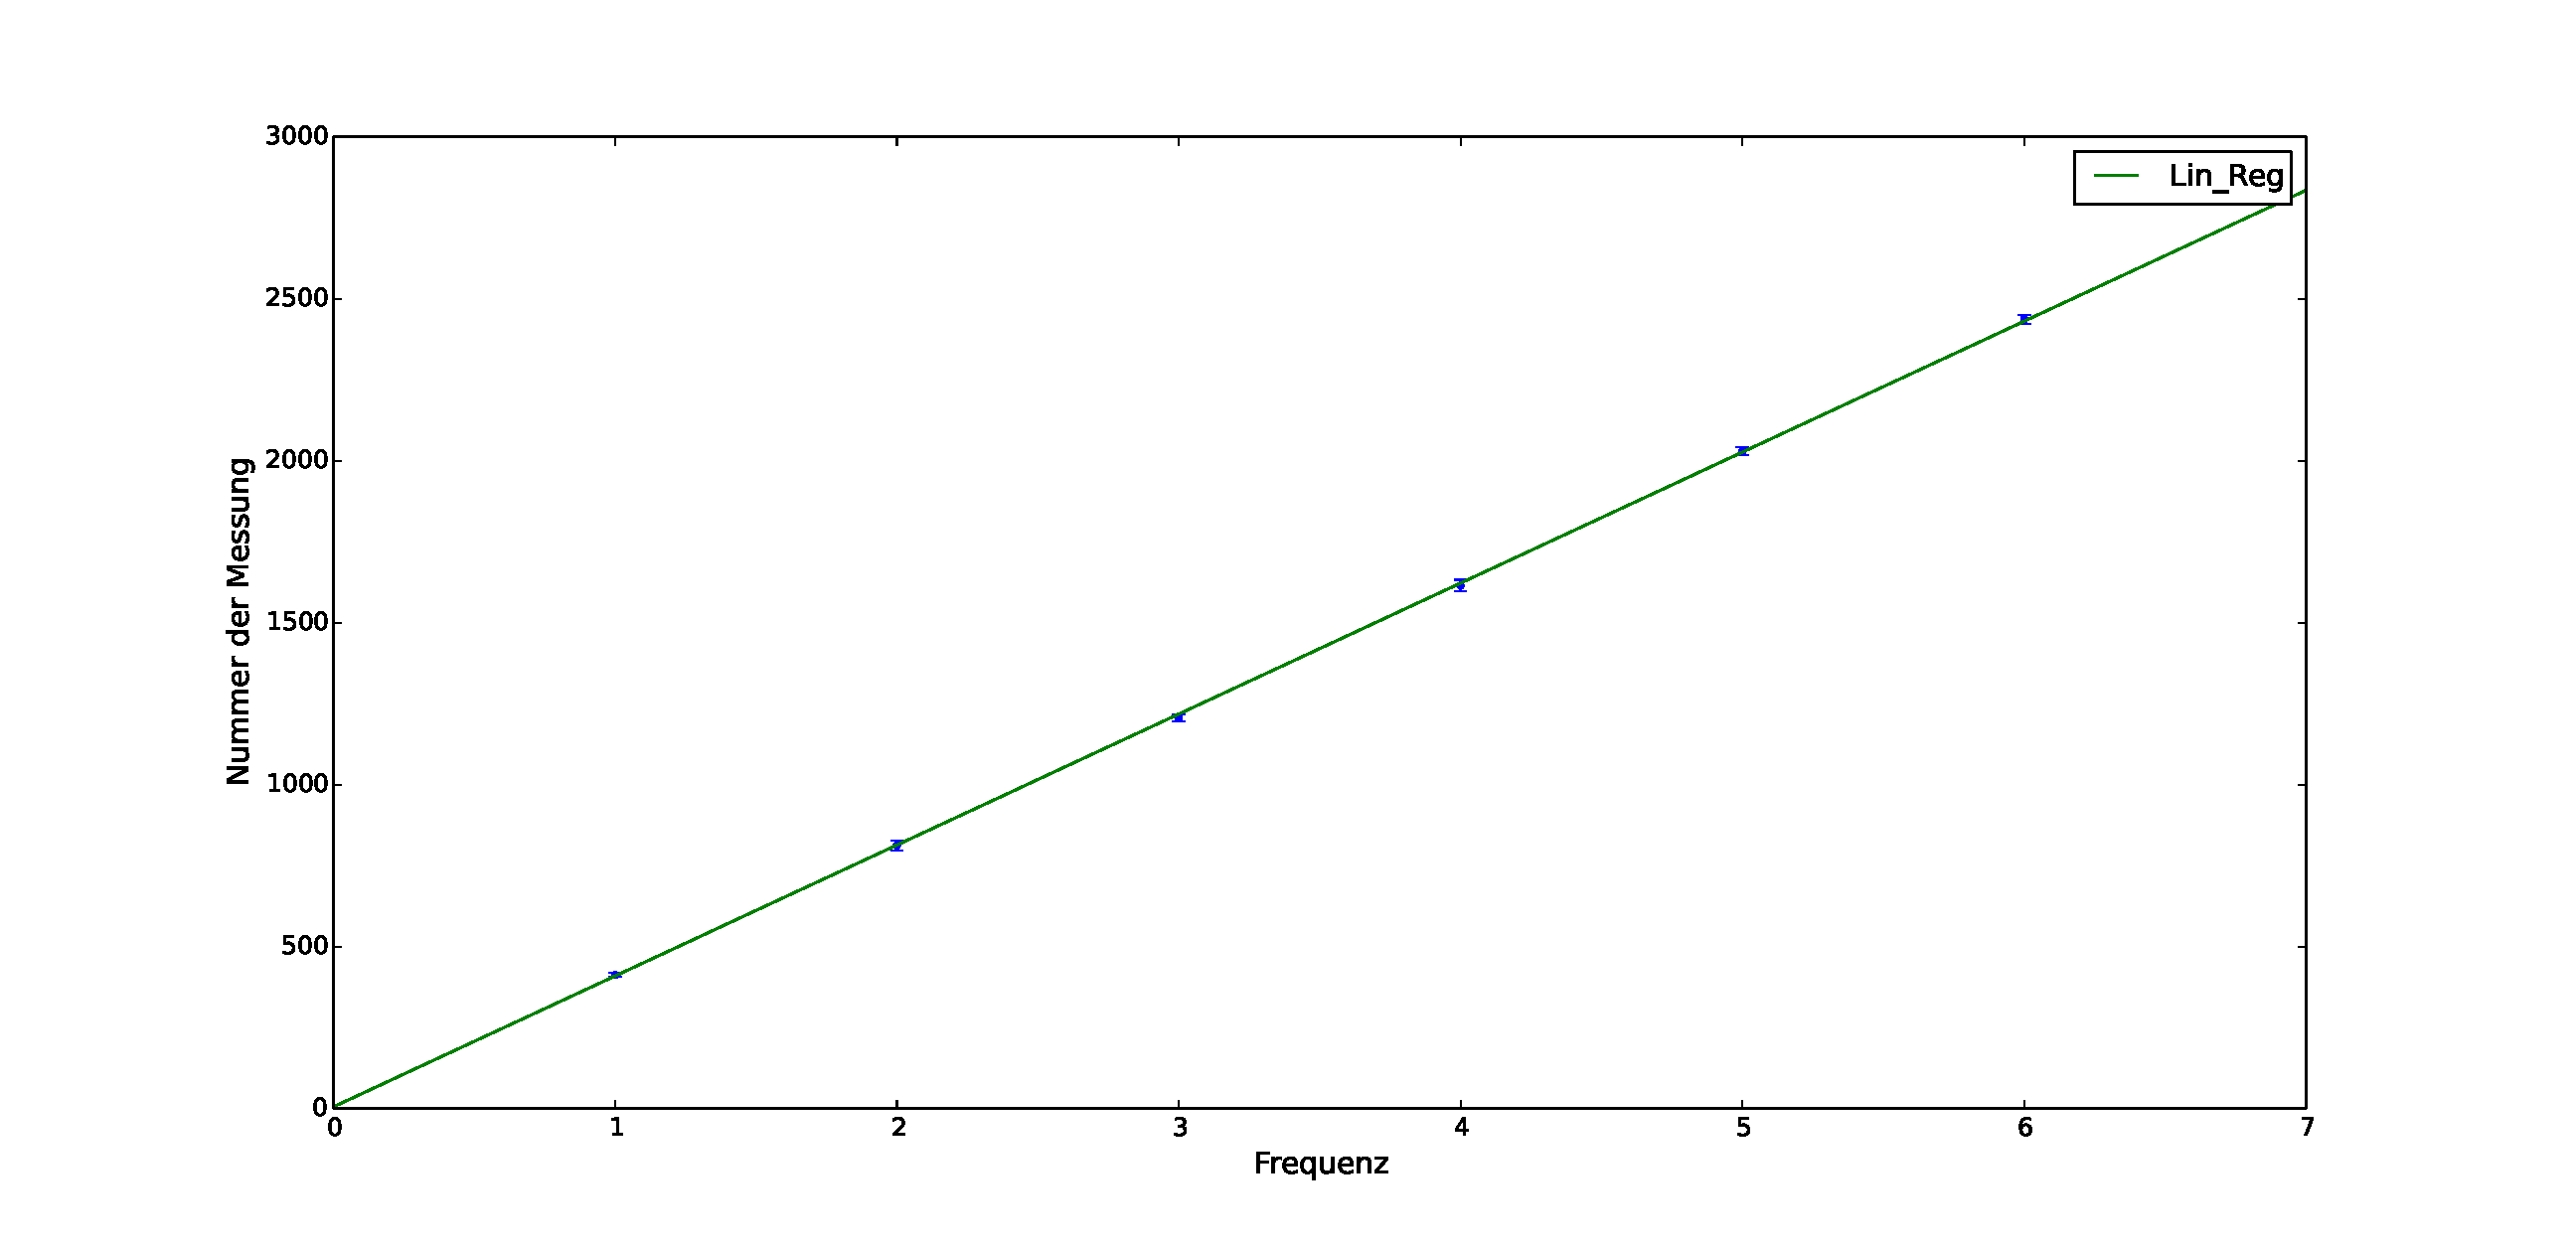
\includegraphics[scale=0.3]{Bilder/linreg_variation.eps}
\caption{Lineare Regression, die Steigung gibt $\frac{v_{Schall}}{2\cdot L}$ zurück}
\end{figure}
Mit einem $\chi^2 = 0.43$ ist unsere Anpassung in einem akzeptablen Rahmen. Das spiegelt sich auch in unserem Residuenplot wieder:
\begin{figure}[H]
\centering
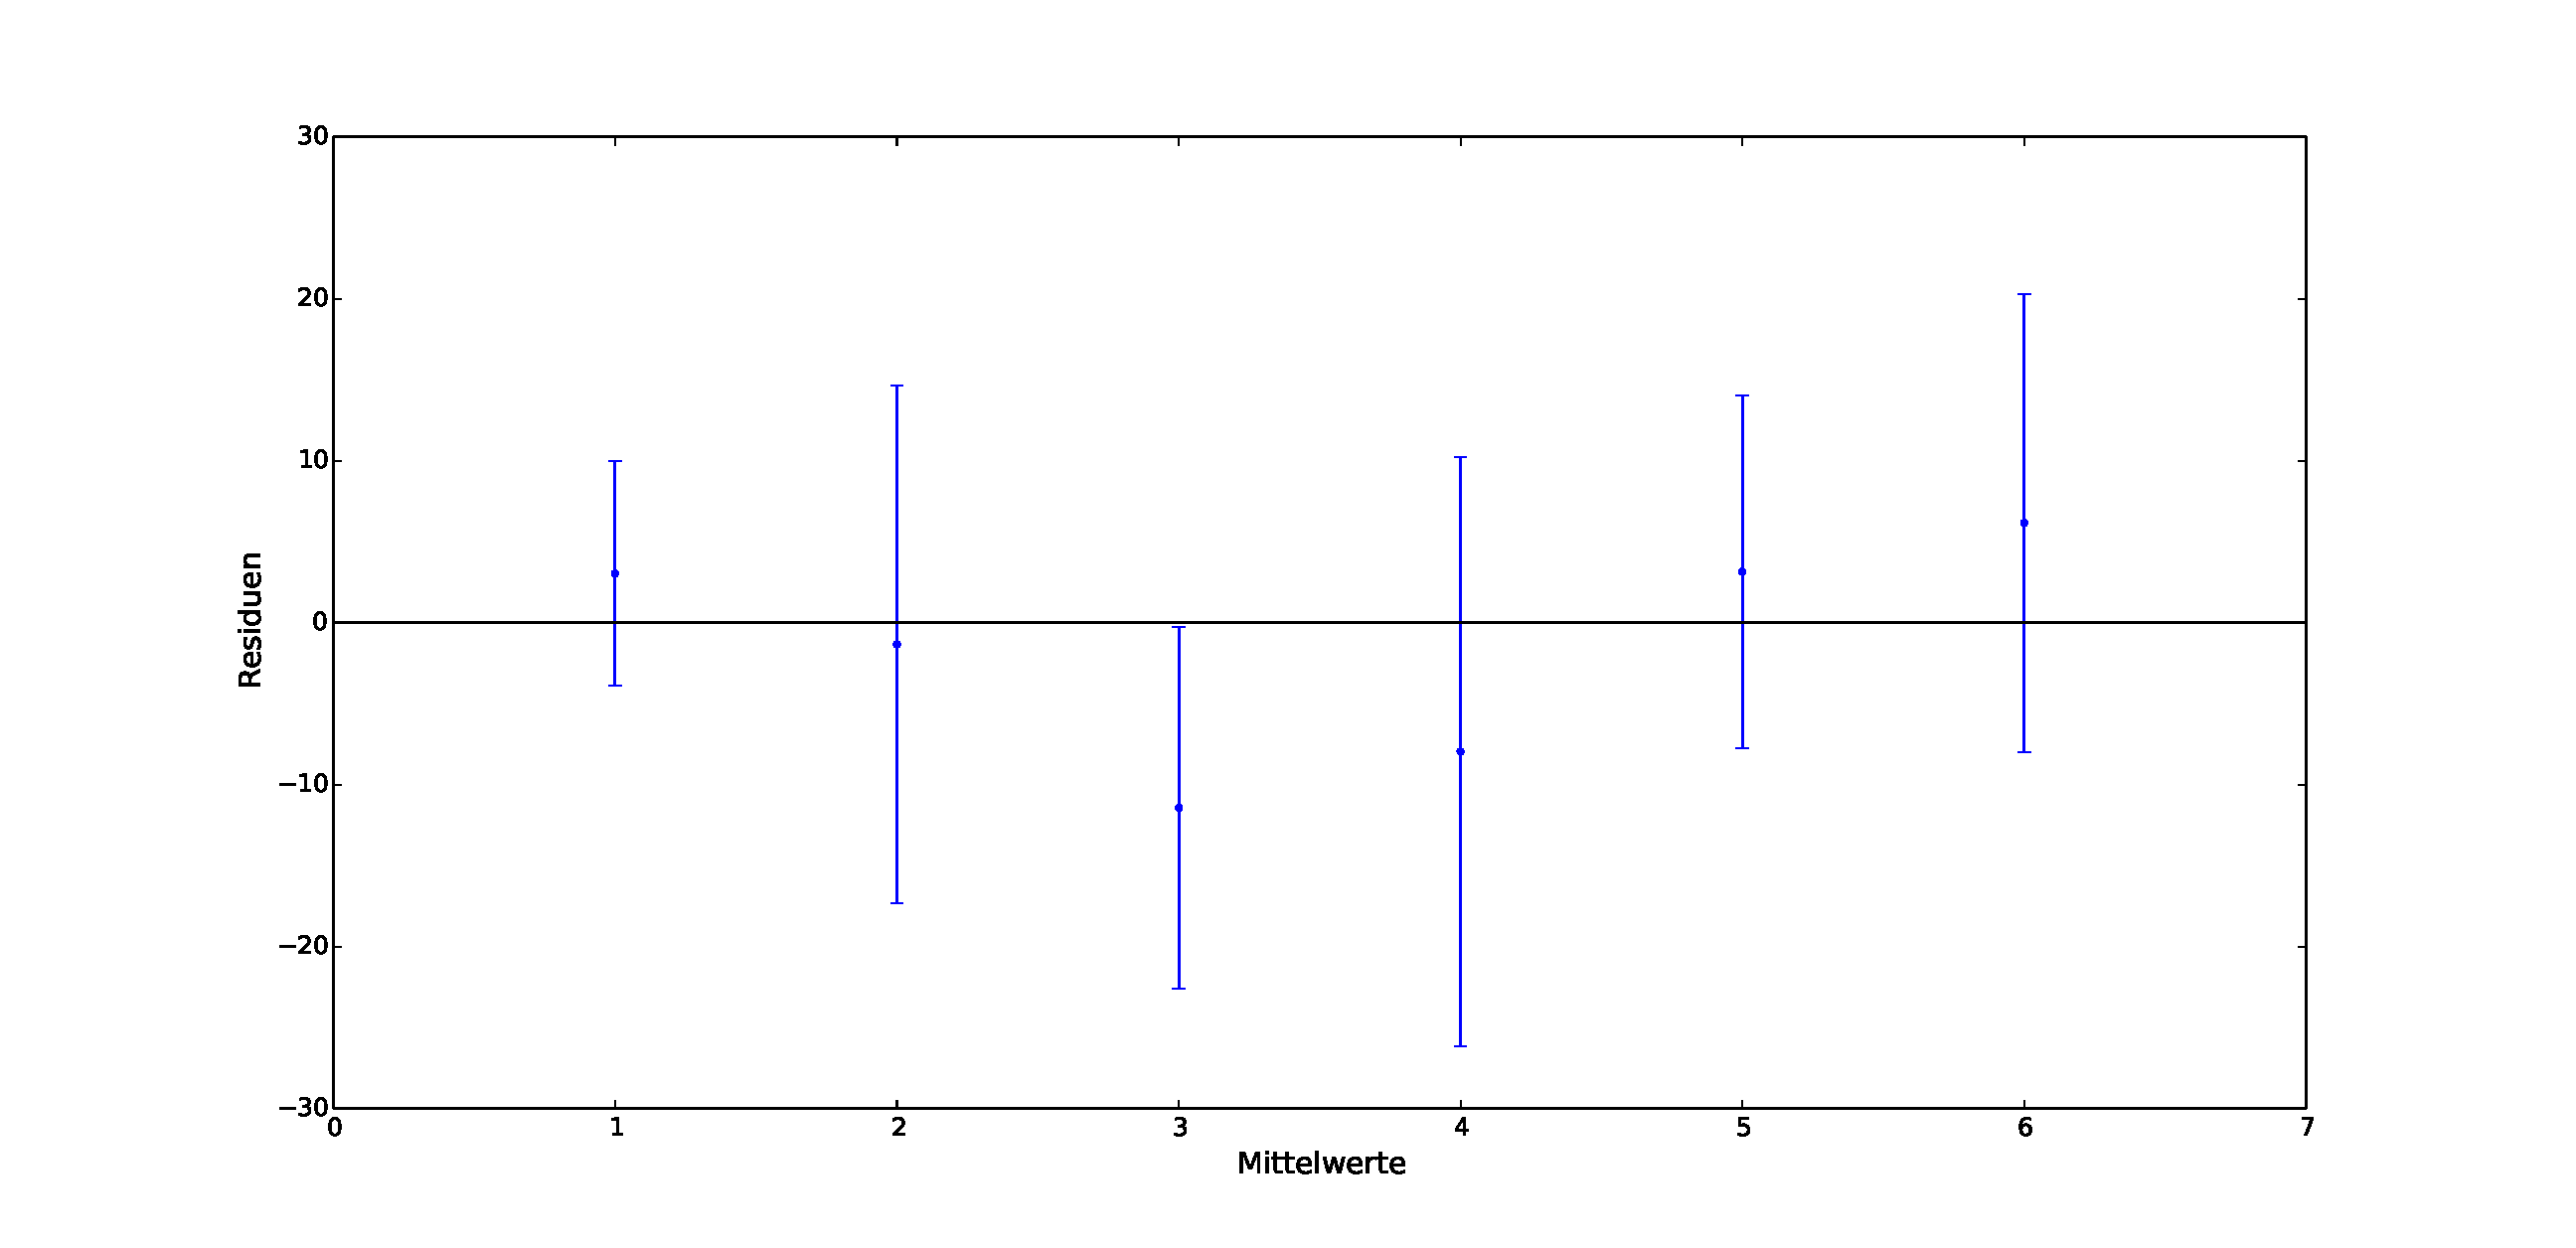
\includegraphics[scale=0.3]{Bilder/Residuen_Variation_Frequenzen.eps}
\caption{Residuenplot (Werte-Fit), zeigt Güte der Anpassung}
\end{figure}
Die Residuen streuen gleichverteilt um 0. 5 von 6 Werten schneiden die Nulllinie mit ihren Fehlerbalken, das entspricht $83.3\%$ der Werte die innerhalb von einem $\sigma$ den Sollwert schneiden. 
Die Steigung der Linearen Regression gibt uns die Schallgeschwindigkeit mit dem Faktor $\frac{1}{2\cdot L}$ wieder, wie auch schon in
\begin{equation}
f_n = \frac{n\cdot v}{2\cdot L}
\end{equation}
zu sehen ist.
Die Fehler auf die Längenmessung und die Fehler auf die Mittelwerte unserer Resonanzfrequenzen haben wir wie folgt fortgepflanzt:
\begin{equation}
\sigma_v = \sqrt{f_R^2\cdot\sigma_{\lambda}^2 + \lambda^2\cdot\sigma_f^2}
\end{equation}
mit
\begin{equation}
\sigma_{\lambda} = \sigma_{\bar{M}}\cdot\sqrt{2}
\end{equation}
$\bar{M}$ und $\sigma_{\bar{M}}$ haben wir erhalten durch:
\begin{equation}
\bar{M} = \frac{\sum_{i=1}^{N}{X_i}}{N}
\end{equation}
und
\begin{equation}
\sigma_{\bar{M}}=\frac{\sqrt{\frac{\sum_{i=1}^{N}({X_i-\bar{M}})^2}{N-1}}}{\sqrt{N}}
\end{equation}
Nach der Korrektur erhalten wir einen Wert für $v$ von
\begin{equation}
v = 343.46 \pm 2.08\,\frac{m}{s}
\end{equation}.

\subsection{Fazit}
Unser Wert für $v_{Schall}$ liegt innerhalb eines $\sigma$ Abstand zum Literaturwert (bei $T = 20^{\circ}\,$C) $v_{lit}=343\,\frac{m}{s}$. Unsere Fehlerabschätzungen führen zu einem relativen Fehler auf $v$ von $0.58\%$, was, zusammen mit unserem $\chi^2 = 0.43$ und Residuenplot, der keine Systematiken aufweist, sondern eine gleichverteilte Streuung um 0 zeigt, auf eine sehr präzise Messung schließen lässt, mit der wir als Gruppe zufrieden sind.
\newpage
\section{Schallgeschwindigkeit in Festkörpern}
\subsection{Versuchsbeschreibung}
%Kurze Darstellung der physikalischen Grundlagen und Ziele der Versuche, die zum Verständnis des Versuches/Protokolls benötigt werden. (max. 1 Seite)
Die Ausbreitungsgeschwindigkeit v in einem Festkörper kann über den Elastizitätsmodul und die Dichte des Materials bestimmt werden:
\begin{equation}
v=\sqrt{\frac{E}{\rho}}
\end{equation}
Mit $v=f\cdot \lambda$ und $\lambda=2L$ ergibt sich für den Elastizitätsmodul:
\begin{equation}
E= \rho\cdot f^2\cdot 4L^2
\end{equation}

\subsection{Versuchsaufbau und Durchführung}
%Genaue Beschreibung der verwendeten Aufbauten unter Verwendung von Skizzen oder Photos
%Beschreibung der Messwerterfassungseinstellungen (eingestellte Messzeiten, Messbedingungen, Trigger, Anzahl der Messungen) und der Durchführung der Versuche. (max. 1 Seite)\newline
Zur Berechnung des Elastizitätsmoduls wurden 4 Stäbe mit Stativmaterial so eingespannt, dass diese nur in der Mitte einen Kontaktpunkt mit der Klemme haben (siehe Abbildung \ref{Stange}). Da wir dort einen Schwingunsknoten erwarten, können wir Verlusste durch die Aufhängung im Folgenden vernachlässigen. Nachdem wir die Massen der zylinderförmigen Stäbe bestimmt hatten und diese befestigt wurden, haben wir mehrfach die Dicken der Stangen an unterschiedlichen Stellen und die Längen gemessen. Des Weiteren konnten wir $\rho$ dann aus $\rho=\frac{M}{V}=\frac{4\cdot M}{L\cdot \pi D^2}$ bestimmen.\newline
Zur Messung der Eigenfrequenz haben wir auf das eine Stabende mit einem Gummihammer geschlagen, an dem anderen Ende wurde ein Mikrofon in ca. 5mm Entfernung angebracht, das wir mit Cassy verbunden haben. Dort konnten wir mittels Fast-Fourier-Transformation die Frequenzen bestimmen, wobei wir hier nur Grundschwingungen betrachtet haben.
\begin{figure}[H]
\centering
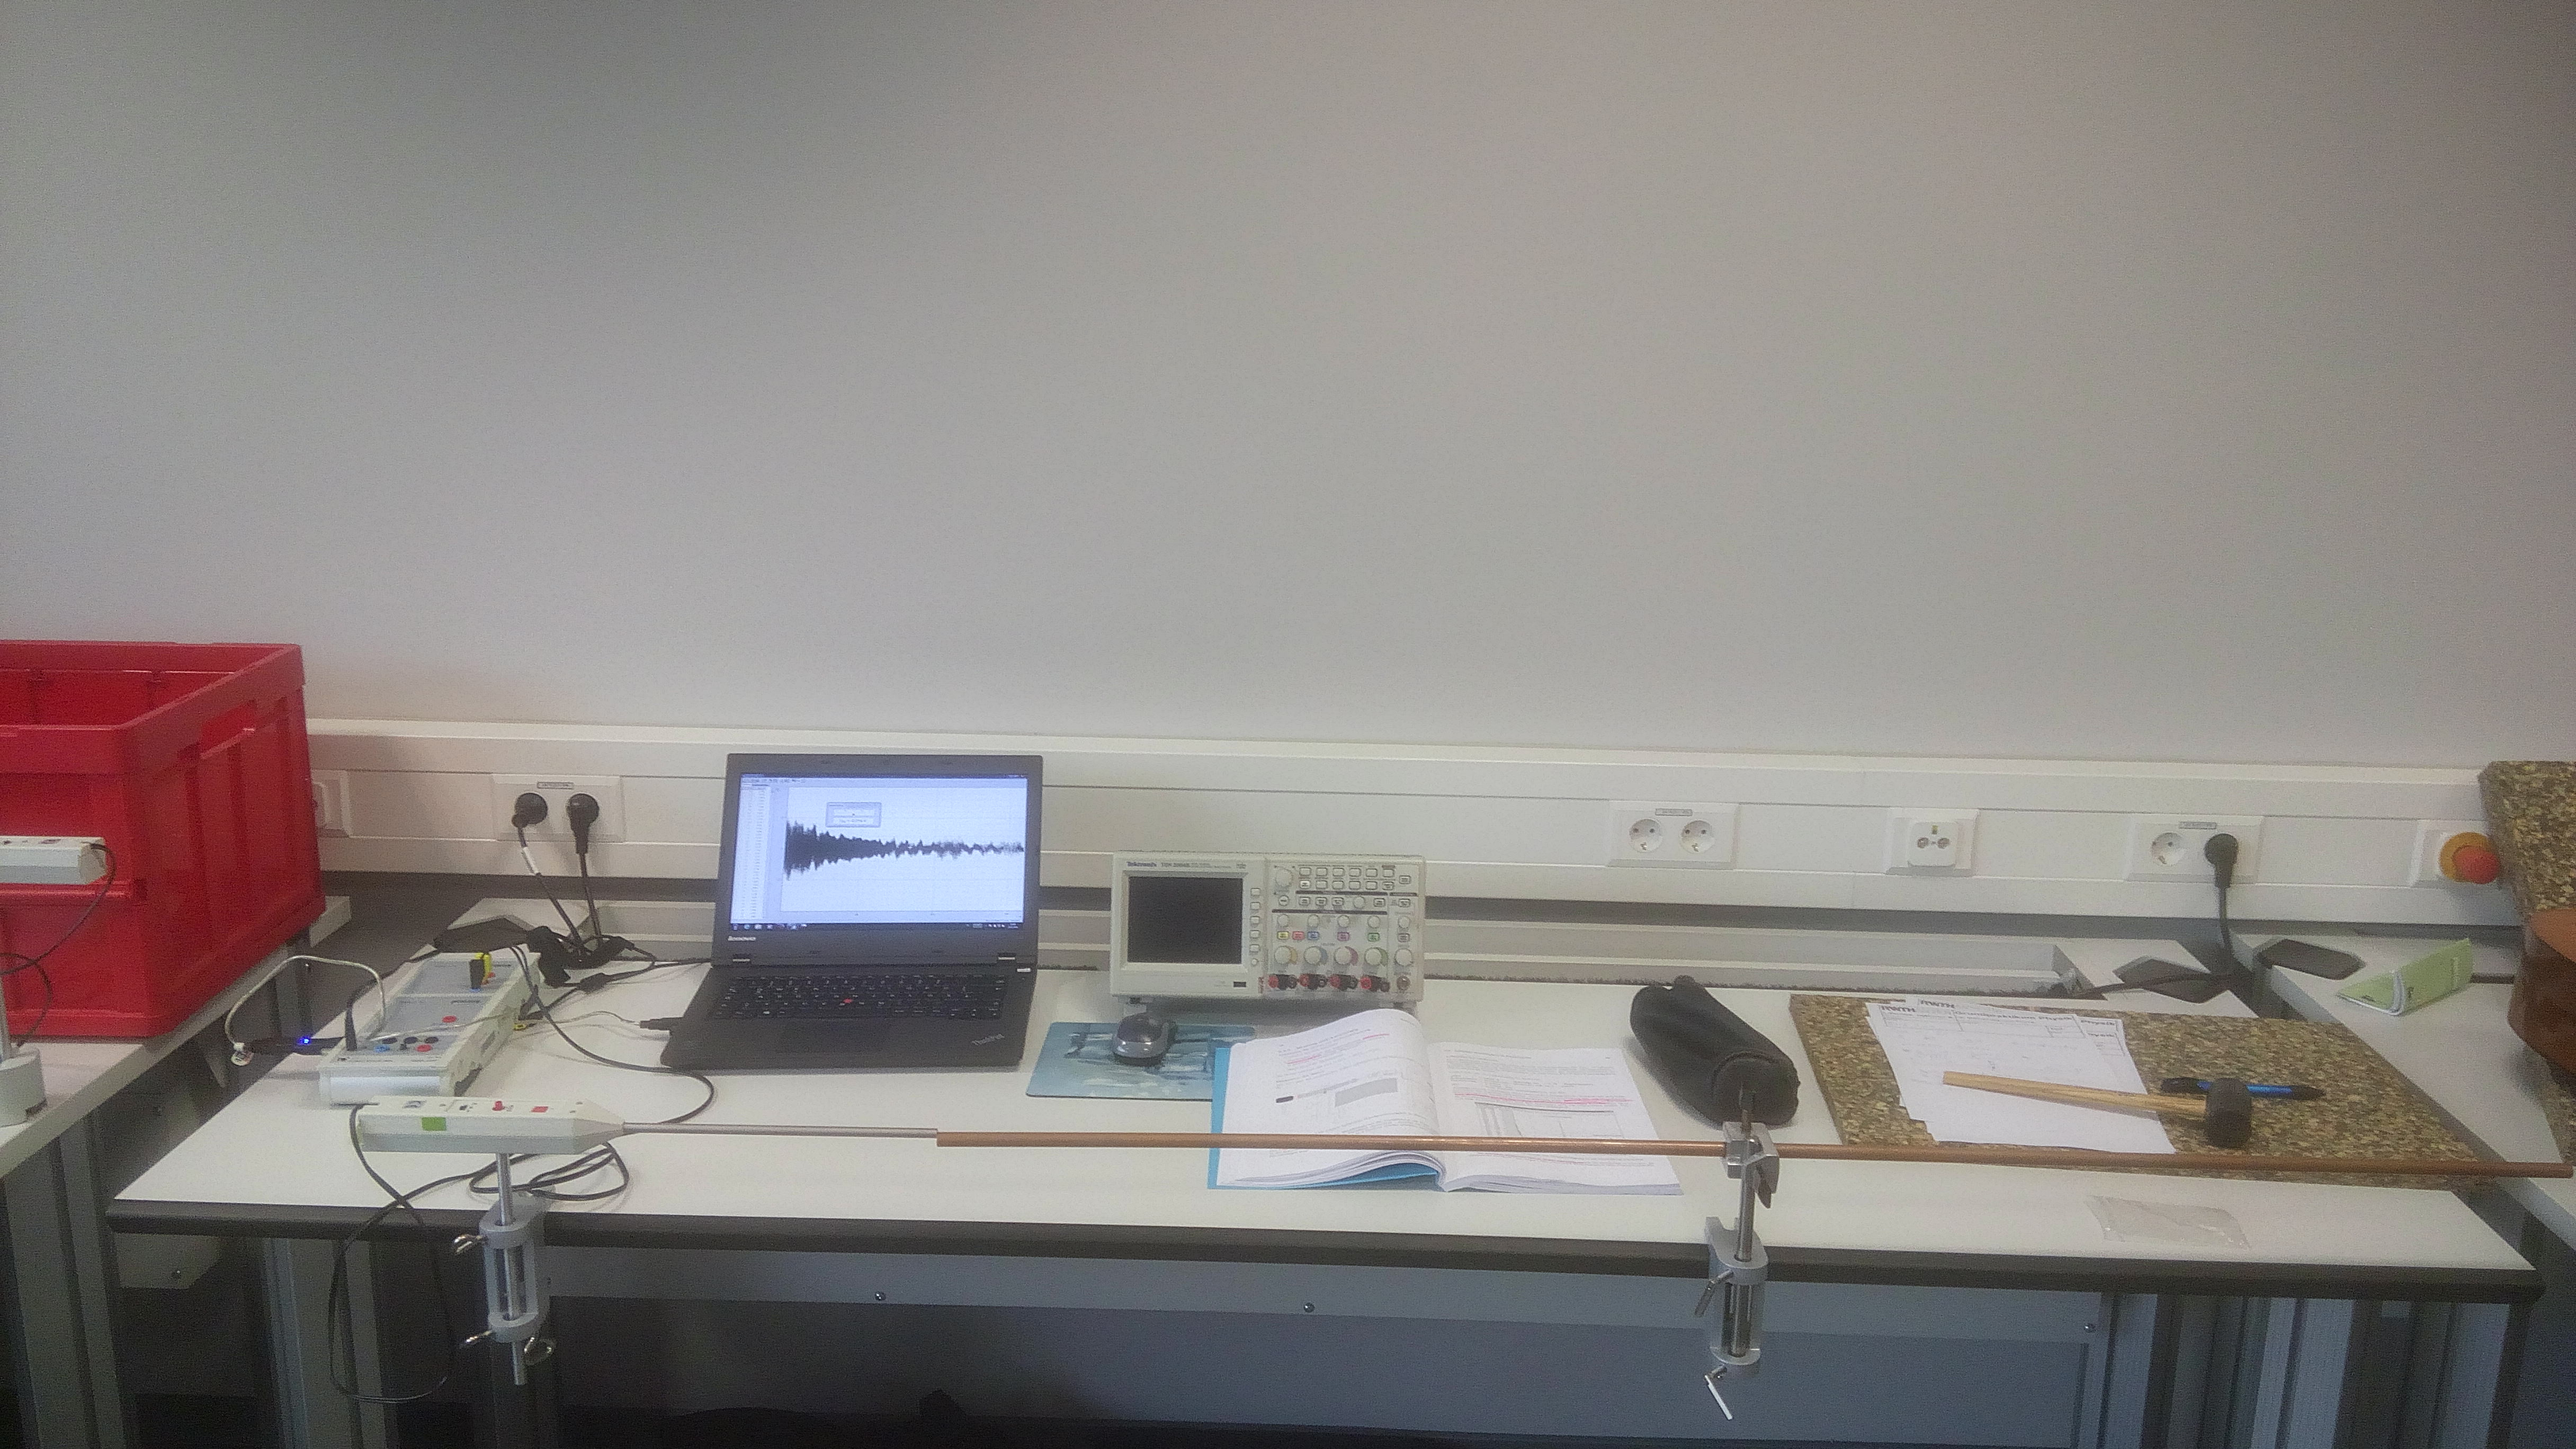
\includegraphics[scale=0.093]{Bilder/Arbeitsplatz_Stange.jpg}
\caption{Übersicht Arbeitsplatz}
\end{figure}

\begin{figure}[H]
\centering
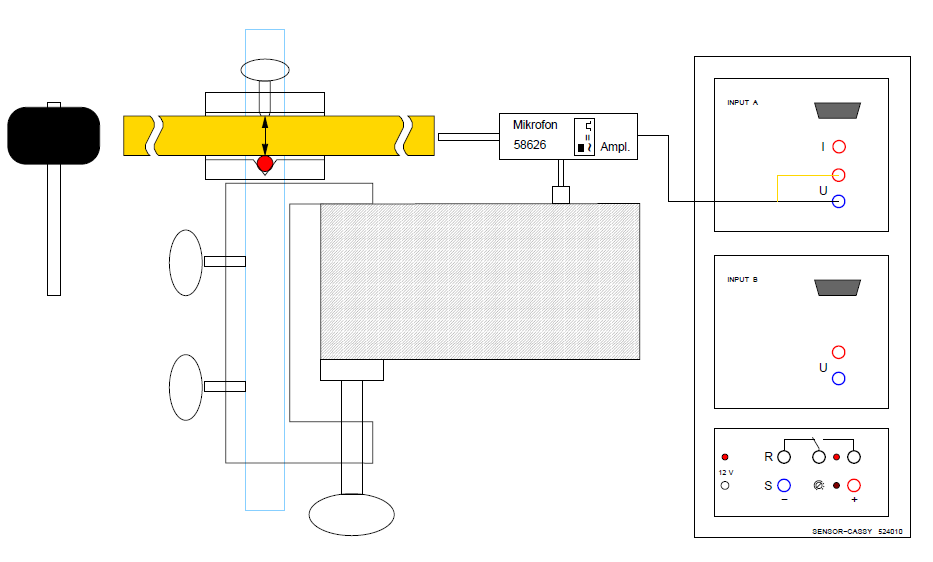
\includegraphics[scale=0.6]{Bilder/Versuchsaufbau_Skript.PNG}
\caption{Versuchsaufbau}
\label{Stange}
\end{figure}


\subsubsection{Messwerterfassungseinstellungen}
\begin{center}
\begin{tabular}{c|c}
Messbereich jeweils Messung 1-5 & -0.3..0.3V\\ 
\hline
Messbereich jeweils Messung 6-10 & -1.0..1.0V\\ 
\hline
Messintervall & 10$\mu$s \\ 
\hline
Messpunkte & 16000 \\ 
\hline
Messzeit & 1.6s \\ 
\end{tabular} 
\end{center}
Der Messbereich wurde hier immer nach der fünften Messung geändert, weil wir bei den Schlägen 6 bis 10 mit dem Stabende fester geschlagen haben und so die Amplituden in Cassy größer als der Messbereich wurden.
\subsubsection{Geräteübersicht}
\begin{itemize}
\item 4 Metallstangen
\item 1 Laptop
\item 1 Sensor-Cassy
\item 1 Universalmikrofon
\item 1 Gummi-Hammer
\item 1 Maßband
\item 1 Mikrometermaß
\item 1 Analysewaage
\item Stativzubehör
\end{itemize}
\subsection{Versuchsauswertung}

\subsubsection{Rohdaten}

\begin{table}[H]\centering
\caption{Masse m und Länge L der Stangen}
\begin{tabular}{c|cccc}
& Stange 1 & Stange 2 & Stange 3 & Stange 4 \\ 
\hline
m in kg & 1.3019 & 1.3249 & 1.1570 & 1.2364 \\ 
L in m & 1.299  & 1.50 & 1.301 & 1.299 \\ 
\end{tabular} 
\end{table}
Der statistische Fehler auf die Einzelmessung ergibt sich zu:
\begin{align*}
\sigma_m=0.0001\,kg\\
\sigma_l=0.5\cdot10^{-2}\,m
\end{align*}
\begin{equation}
\sigma_i=\sqrt{\frac{\sum_i^n(x_i-x_{mean})^2}{n-1}}
\end{equation}

\begin{table}[H]\centering
\caption{Die Dicke d der Stangen (in mm) wurde an 5 verschiedenen Stellen gemessen.}
\begin{tabular}{c|cccc}
 & Stange 1 & Stange 2 & Stange 3 & Stange 4 \\ 
 \hline
$d_1$ & $12.47$ & $12.01$ & $11.97$ & $11.97$ \\ 
$d_2$ & $12.47$ & $12.00$ & $11.97$ & $11.97$ \\ 
$d_3$ & $12.47$ & $11.99$ & $11.95$ & $12.00$ \\ 
$d_4$ & $12.47$ & $11.99$ & $11.97$ & $11.97$ \\ 
$d_5$ & $12.47$ & $12.01$ & $11.96$ & $11.98$ \\ 
\hline
$d_{mean}$ & $12.47$ & 12.00 & 11.96 & 1198 \\ 
$\sigma_{d_{mean}}$ & $0.00$ & $4.47\cdot 10^{-3}$ & $4.00\cdot 10^{-3}$ & $5.83\cdot 10^{-3}$ \\ 
\end{tabular} 
\end{table}

Die Frequenzen f (in Hz) wurden mittels Fast-Fourier-Transformation und Peakschwerpunktbestimmung aus Cassy abgelesen.

\begin{figure}[H]
\centering
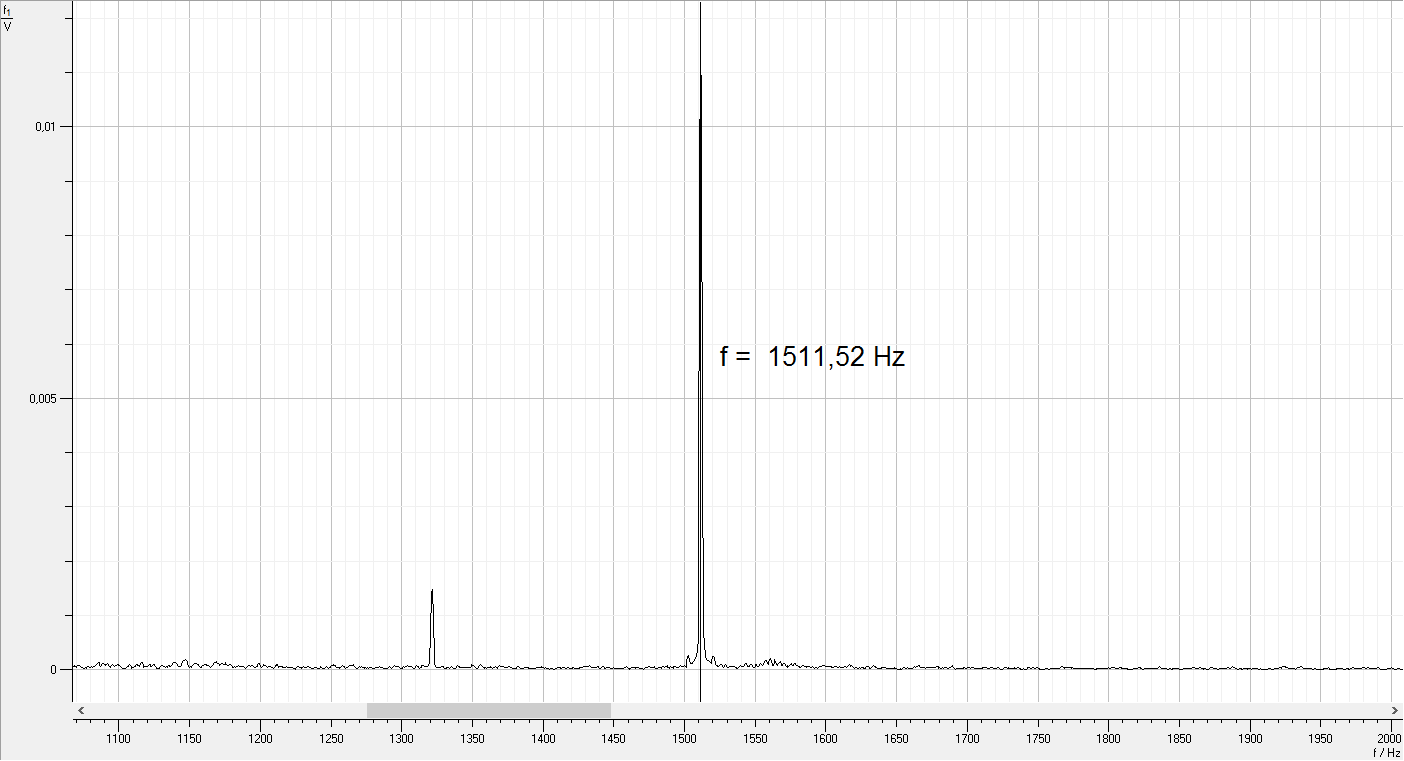
\includegraphics[scale=0.43]{Bilder/Beispiel_Cassy_Cu.png}
\caption{Beispiel zu Frequenz aus FFT ablesen (Stange 1)}
\end{figure}

\begin{table}[H]\centering
\caption{Frequenzen aus der FFT für alle 4 Stangen}
\begin{tabular}{c|cccc}
 & Stange 1 & Stange 2 & Stange 3 & Stange 4 \\ 
 \hline
$f_1$ & 1511.52 & 1728.17 & 1884.03 & 1348.48 \\ 
$f_2$ & 1511.54 & 1728.18 & 1884.04 & 1348.50 \\ 
$f_3$ & 1511.52 & 1728.18 & 1884.07 & 1348.49 \\ 
$f_4$ & 1511.53 & 1728.19 & 1884.06 & 1348.50 \\ 
$f_5$ & 1511.51 & 1728.18 & 1884.09 & 1348.50 \\ 
$f_6$ & 1511.53 & 1728.17 & 1884.11 & 1348.54 \\ 
$f_7$ & 1511.54 & 1728.18 & 1884.13 & 1348.55 \\ 
$f_8$ & 1511.51 & 1728.20 & 1884.14 & 1348.55 \\ 
$f_9$ & 1511.51 & 1728.19 & 1884.13 & 1348.52 \\ 
$f_{10}$ & 1511.48 & 1728.20 & 1884.14 & 1348.52 \\
\hline 
$f_{mean}$ & 1511.52 & 1728.18 &  1884.09 & 1348.52 \\ 
$\sigma_{f_{mean}}$ & 0.006 & 0.003 & 0.013 & 0.008 \\ 
\end{tabular} 
\end{table}

Dabei wurden die Mittelwerte mit ihren Fehlern für die Dicke der Stangen und für die Frequenzen aus
\begin{align}
x_{mean}=\frac{1}{n} \cdot \sum_i^n x_i\\
\sigma_{x_{mean}}=\frac{\sigma_i}{\sqrt{n}}
\end{align}
bestimmt.
\subsubsection{Transformation der Rohdaten und Analyse}
%Transformation der Rohdaten und Modellanpassung. (1 Seite)\\
Nachdem alle Werte in Python eingelesen wurden, haben wir die Dichten der Metallstäbe mit
\begin{equation}
\rho=\frac{M}{V}=\frac{4\cdot M}{L\cdot \pi D^2}
\end{equation}
ausgerechnet.\newline
Die Fehler auf die Dichten $\sigma_{\rho}$ ergeben sich nach Fehlerfortpflanzung zu:
\begin{equation}
\sigma_{\rho}=\sqrt{(\frac{\sigma_m}{m})^2+(\frac{\sigma_L}{L})^2+(2\cdot \frac{\sigma_d}{d})^2}\cdot \rho
\end{equation}
wobei hier nur noch mit den Mittelwerten für die Dicken gerechnet wurde, also nehmen wir einen homogenen Zylinder mit der Durchschnittsdicke $d_{mean}$ an.

\begin{table}[H]\centering
\caption{Ergebnisse der Dichten mit ihren Fehlern}
\begin{tabular}{c|cccc}
  & Stange 1 & Stange 2 & Stange 3 & Stange 4 \\ 
  \hline
$\rho$ in $\frac{kg}{m^3}$ & 8206.3 & 7809.3 & 7910.7 & 8446.8 \\ 
$\sigma_{\rho}$ in $\frac{kg}{m^3}$ & 31.6 & 26.7 & 30.9 & 33.9 \\ 
\end{tabular} 
\end{table}

Danach haben wir aus den Mittelwerten der Frequenzen, Dichten und Längen die Elastizitätsmodule der Stangen 1 bis 4 bestimmt:
\begin{equation}
E=4\rho\cdot f^2\cdot  L^2
\end{equation}
mit den Fehlern:
\begin{equation}
\sigma_{E}=\sqrt{(\frac{\sigma_{\rho}}{\rho})^2+(2\cdot \frac{\sigma_L}{L})^2+(2\cdot \frac{\sigma_f}{f})^2}\cdot E
\end{equation}

\begin{table}[H]\centering
\caption{Ergebnisse der Elastizitätsmodule mit Fehler}
\begin{tabular}{c|cccc}
 & Stange 1 & Stange 2 & Stange 3 & Stange 4 \\
\hline 
E in GPa & 126.5 & 209.9 & 190.1 & 103.7 \\ 
$\sigma_E$ in GPa & 1.1 & 1.6 & 1.6 & 0.8 \\ 
\end{tabular} 
\end{table}

Bei der Auswertung der Ergebnisse fiel uns auf, dass Stange 2 und Stange 3 sehr ähnliche Werte für die Dichten und den Elastizitätsmodul haben. Deshalb vermuten wir, dass diese aus ähnlichem oder (fast) gleichen Material bestehen. Nach weiterer Recherche ordnen wir diese beiden Stangen als Eisen ein. Bei der ersten Stange lässt sich sowohl aus E und $\rho$, als auch durch das Aussehen auf Kupfer schließen und bei der vierten Stange analog auf Messing.\newline
Abschließend haben wir aus den Werten die Schallgeschwindigkeiten in den Metallen mit
\begin{align}
v&=\sqrt{\frac{E}{\rho}}\\
\sigma_v&=\sqrt{(\frac{\sigma_f}{f})^2+(\frac{\sigma_L}{L})^2}\cdot v
\end{align}
 bestimmt und diese mit Literaturwerten\footnote{Quelle: Wikipedia} verglichen.

\begin{table}[H]\centering
\caption{Schallgeschwindigkeiten der 4 Metallstäbe mit entsprechenden Literaturwerten}
\begin{tabular}{c|cccc}
 & Stange 1 & Stange 2 & Stange 3 & Stange 4 \\ 
\hline
v in $\frac{m}{s}$ & 3926.9 & 5184.6 & 4902.4 & 3503.4 \\ 
$\sigma_{v}$ in $\frac{m}{s}$ & 15.1 & 17.3 & 18.8 & 13.5 \\ 
daraus resultierendes Material & Kupfer & Eisen & Eisen & Messing \\ 
$v_{Literatur}$ in $\frac{m}{s}$ &$\approx 4660$ & $\approx 5170$ & $\approx 5170$ & $\approx 3500$ \\ 
\end{tabular} 
\end{table}

\subsubsection{Fazit}
%Diskussion der Ergebnisse und Vergleich der erzielten Ergebnisse mit theoretischen Vorhersagen.
Insgesamt konnten wir mit unserer Messung gute Ergebnisse erziehen, die teilweise von den Literaturwerten abweichen. Diese Abweichungen erklären wir uns durch nicht ganz reines, nicht ganz homogenes Material, sowie durch die Zylindernäherung. Außerdem wurde die Temperatur(-Veränderung) außer acht gelassen. Des Weiteren schwanken die Literaturwerte auf verschiedenen Websites und wurden oft nur als Ungefährwerte angegeben, weshalb ein präziser Vergleich nicht möglich ist.
\newpage
\section{Stimmen der Gitarre über Schwebung}
\subsection{Versuchsbeschreibung}
Schlägt man an einer Gitarre 2 Saiten so an, dass sie denselben Ton erzeugen ergibt sich, wenn die Töne nur leicht voneinander abweichen, eine Schwebung. Nur wenn die Töne exakt gleich sind verschwindet die Schwebung. \newline
In diesem Versuch sollte eine Saite einer Gitarre mit Hilfe der Schwebung gestimmt werden.
\subsection{Versuchsaufbau und Durchführung}

Zu aller erst wurden alle Saiten der Gitarre mit einem Stimmgerät gestimmt.  \newline
Daraufhin wurde die Gitarre auf den Tisch gelegt und die Frequenz jeweils mit einem Mikrofon, das über dem Schallloch der Gitarre angebracht war, aufgenommen. Das Signal des Mikrofons wurde mit dem Spannungsmessgerät des Sensor-Cassy vermessen, um schließlich mit Cassy-Lab am Laptop ausgewertet werden zu können.

\begin{figure}[H]
\centering
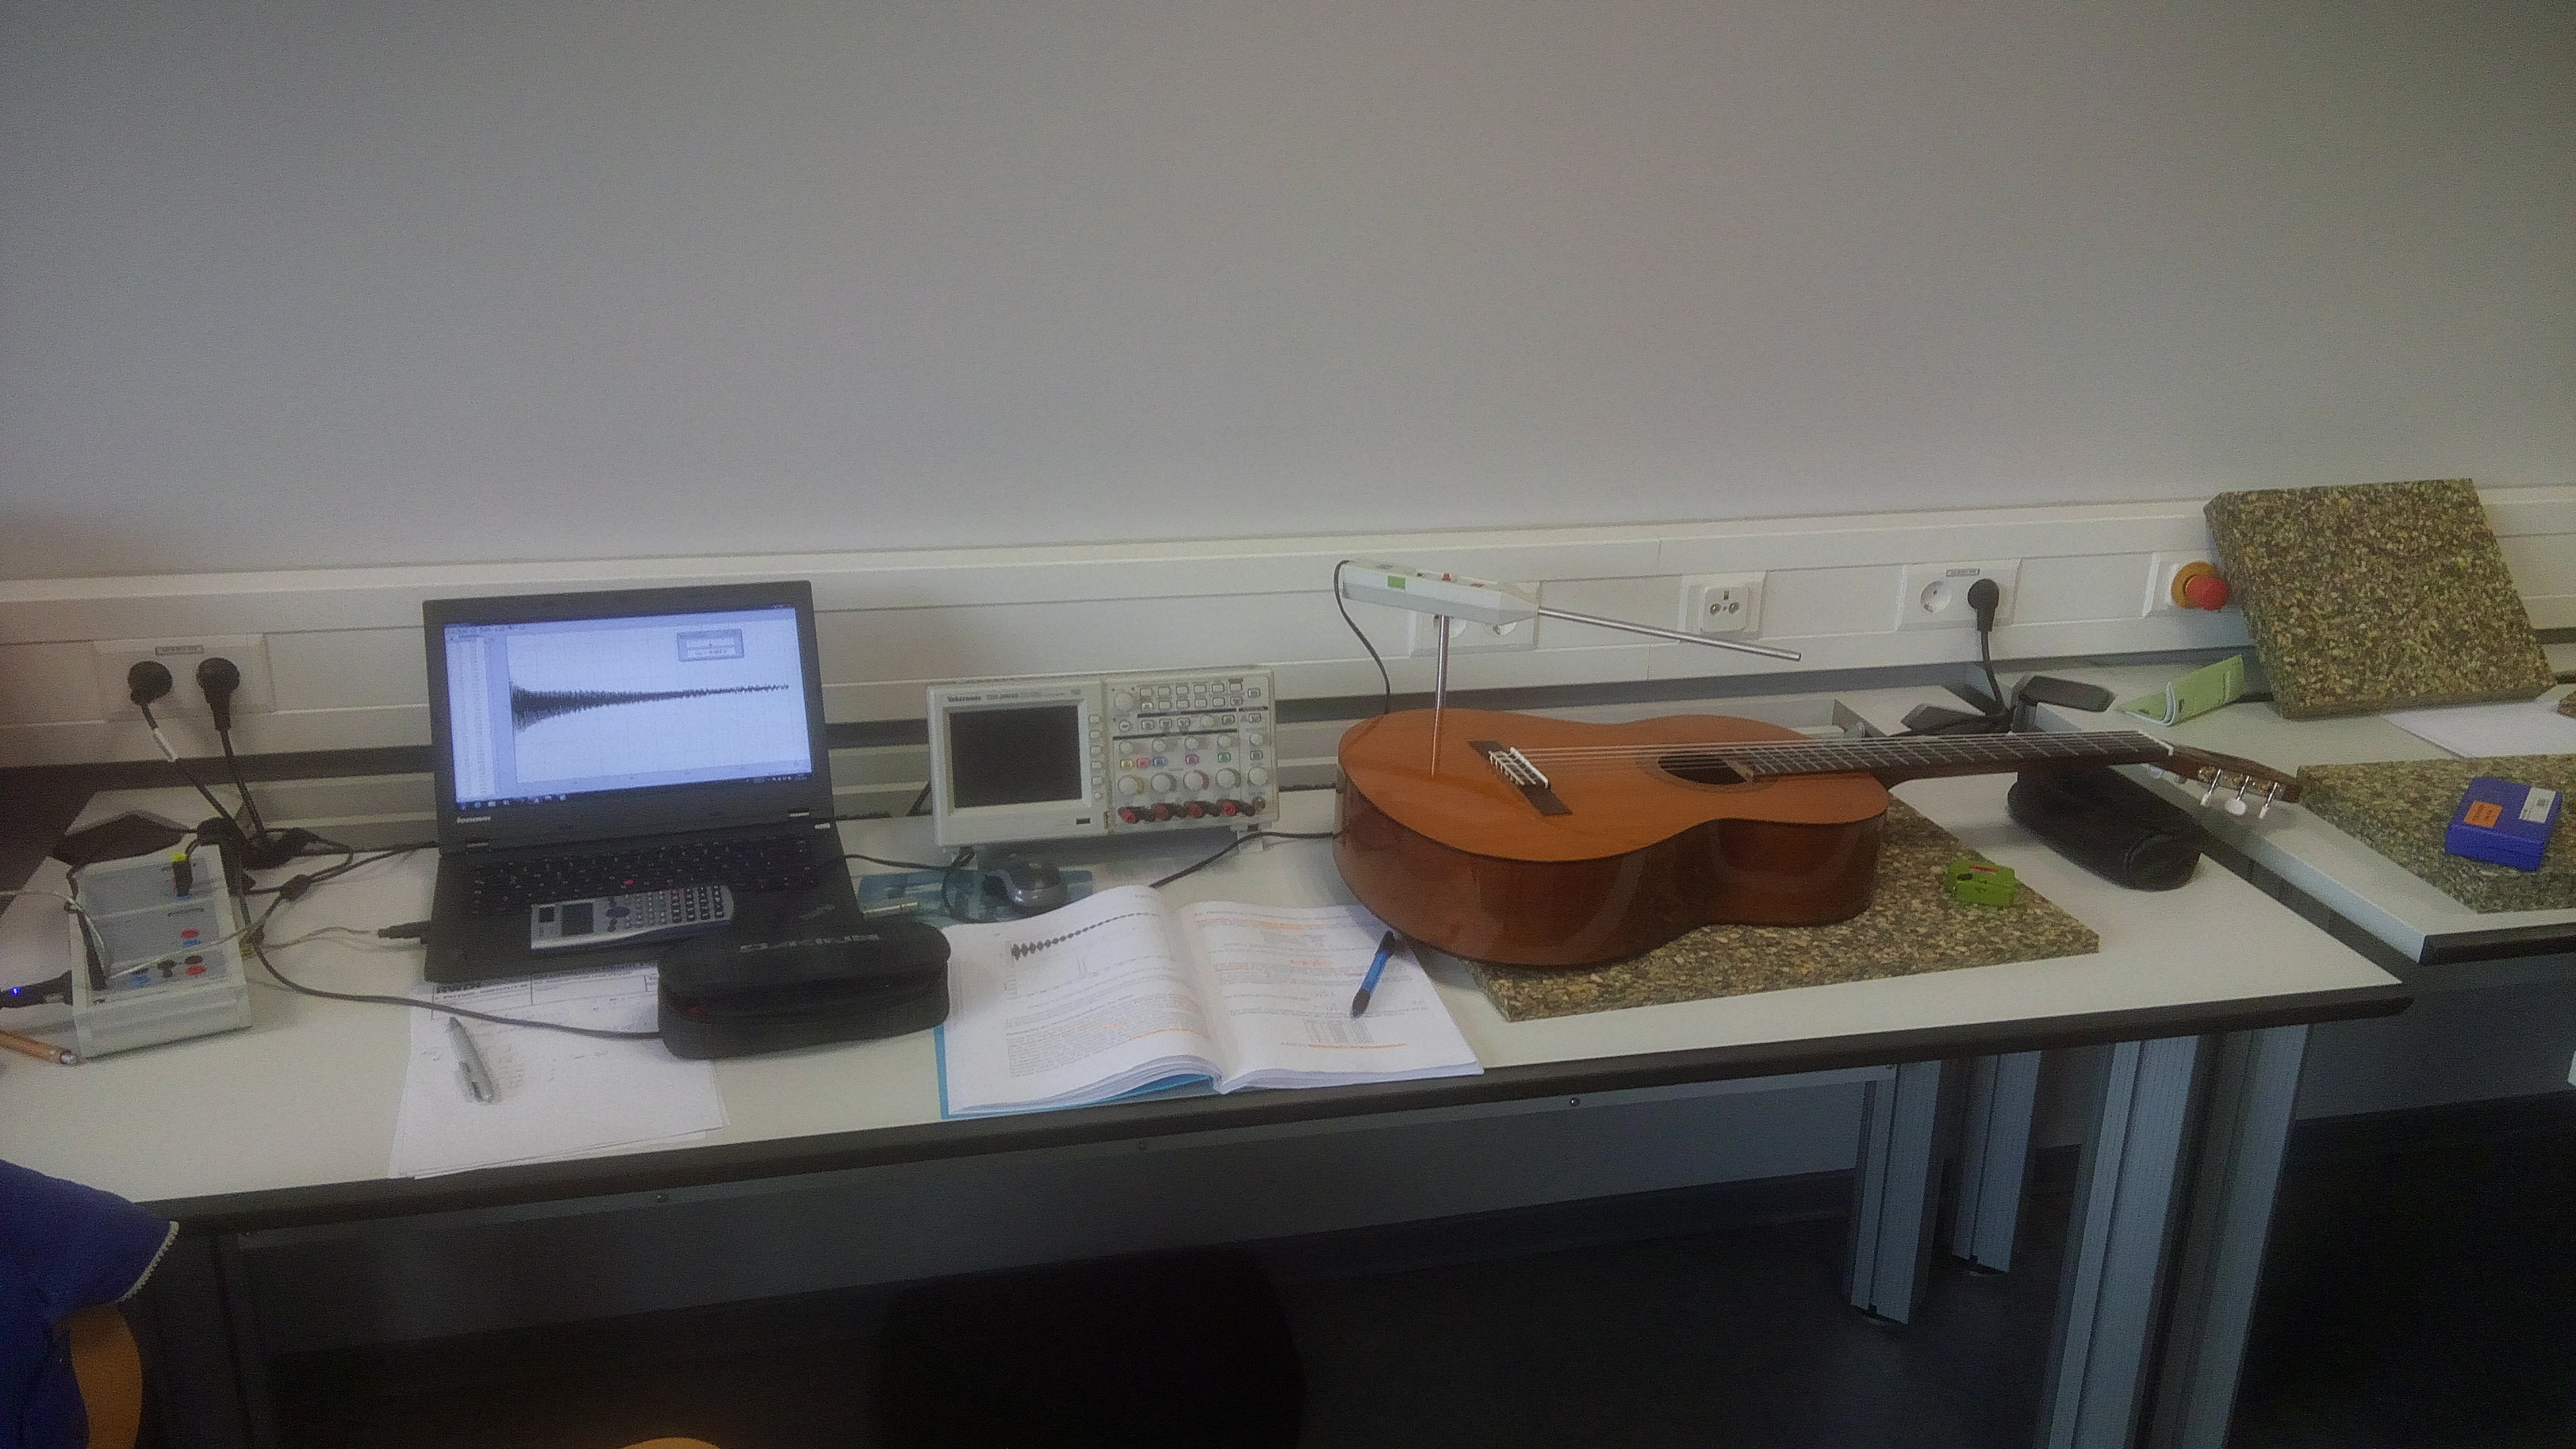
\includegraphics[scale=0.1]{Bilder/IMG_20160323_123920.jpg}
\caption{Versuchsaufbau für Messungen mit der Gitarre. }
\end{figure}


\begin{table}[H]\centering
\caption{Messparameter für Stimmversuche}
\begin{tabular}{c|c}
Parameter & Einstellungen \\ 
\hline
Messintervall & 500 $\mu s$ \\ 
Anzahl Messwerte & 10000 \\ 
Messdauer & 5s \\ 
Trigger & 0.3V \\ 
\end{tabular}
\end{table}
 

Wenn nun die D-Saite leer und die A-Saite im 5. Bund angeschlagen wurde, hörte man denselben Ton ohne Schwebung.

\begin{figure}[H]
\centering
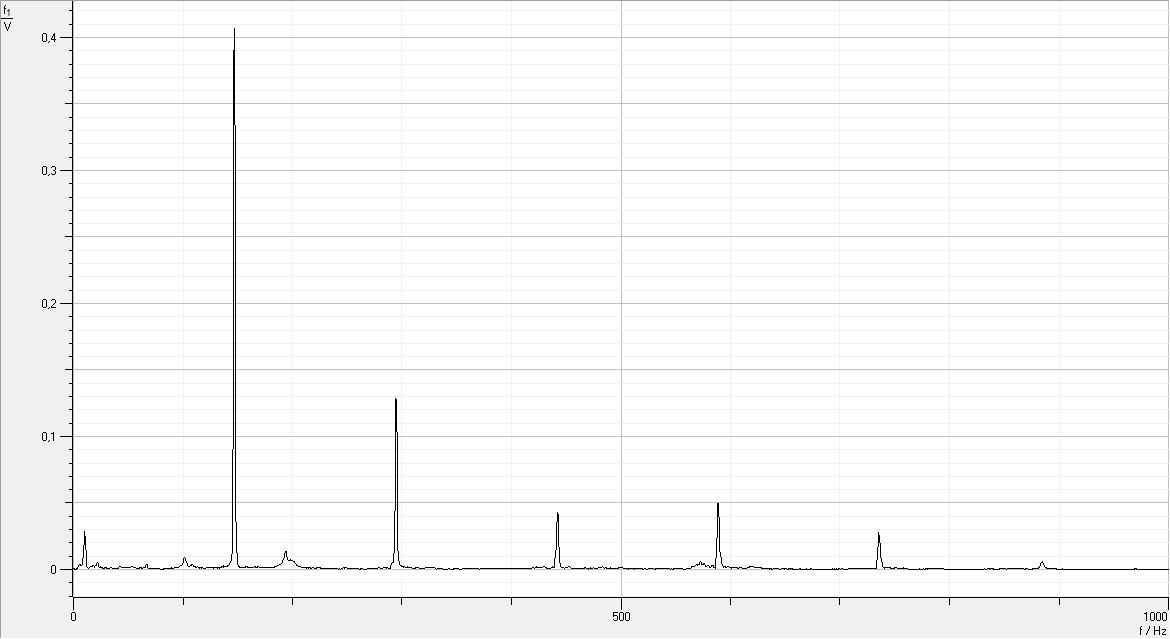
\includegraphics[scale=0.5]{Bilder/Gestimmt_Vorher.png}
\caption{D-Saite leer und A-Saite im 5. Bund nach dem Stimmen mit dem Stimmgerät. Es sind nur jeweils einzelne Peaks sichtbar also keine Schwebung.}
\end{figure}

Als Nächstes wurde die D-Saite so stark verstimmt, dass beim Anschlagen der D-Saite leer und A-Saite im 5. Bund eine deutliche Schwebung zu hören war.

\begin{figure}[H]
\centering
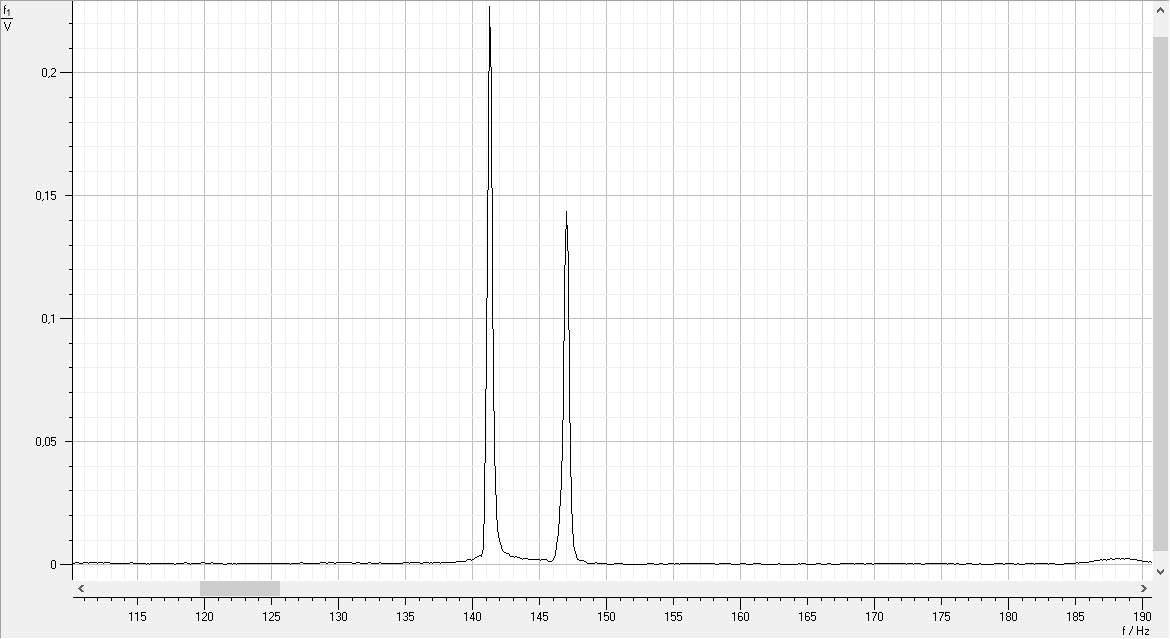
\includegraphics[scale=0.5]{Bilder/Verstimmt.png}
\caption{Verstimmte D-Saite leer und A-Saite im 5. Bund. Es ist eine deutliche Schwebung sichtbar.}
\end{figure}

Die jetzt verstimmte D-Saite wurde daraufhin so weit zurück gedereht bis die Schwebung wieder verschwand.

\begin{figure}[H]
\centering
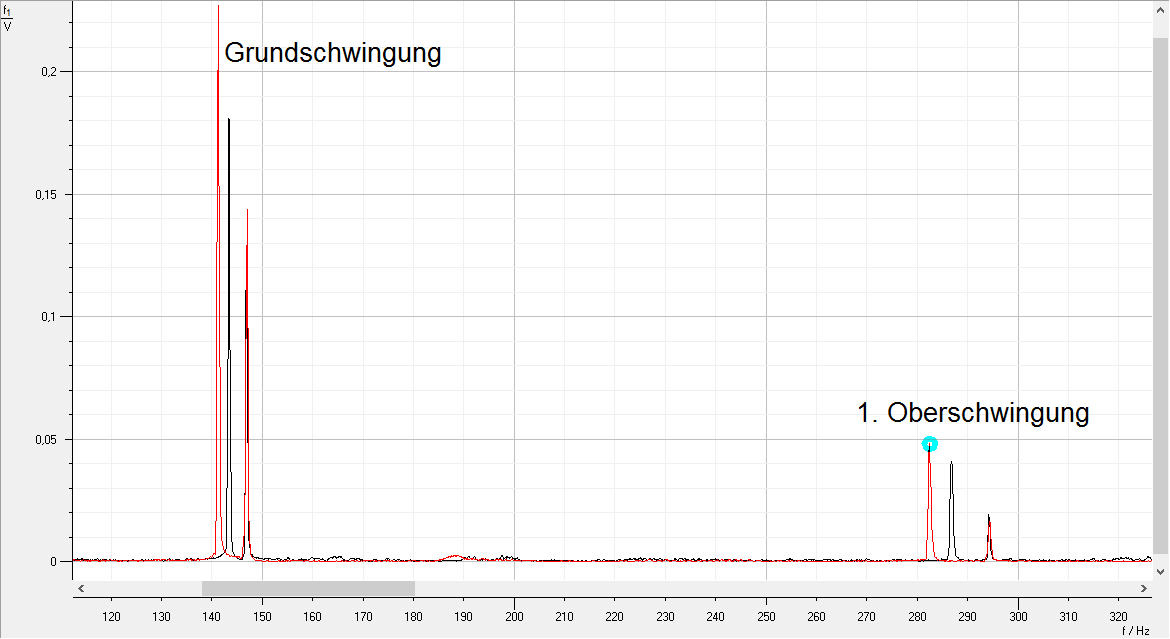
\includegraphics[scale=0.5]{Bilder/Verstimmt_vs_1_stimmen.png}
\caption{Verstimmte D-Saite in rot gegen den ersten Stimmversuch in schwarz. Die Peaks nähern sich. Besonders in der ersten Oberschwingung sieht man die Unterschiede noch deutlicher.}
\end{figure}

\begin{figure}[H]
\centering
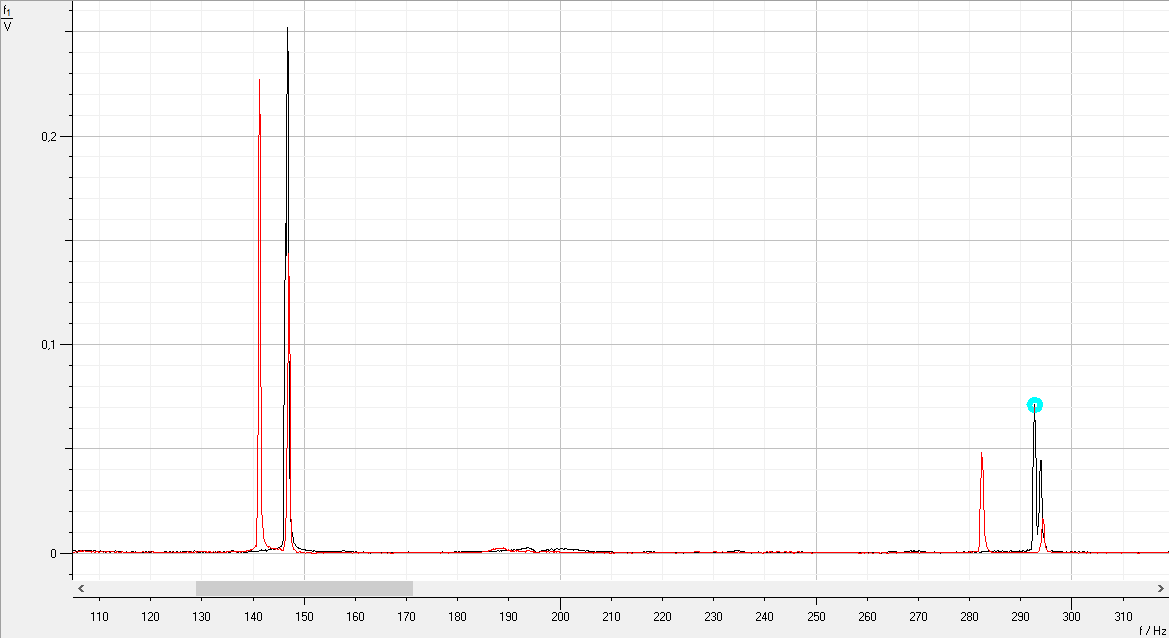
\includegraphics[scale=0.5]{Bilder/Verstimmt_vs_2_stimmen.png}
\caption{Verstimmte D-Saite in rot gegen den zweiten Stimmversuch in schwarz. Bei dem Peak der Grundschwingung ist schon keine Schwebung erkennbar aber in der 1. Oberschwingung sieht man noch eine leichte Schwebung.}
\end{figure}

\begin{figure}[H]
\centering
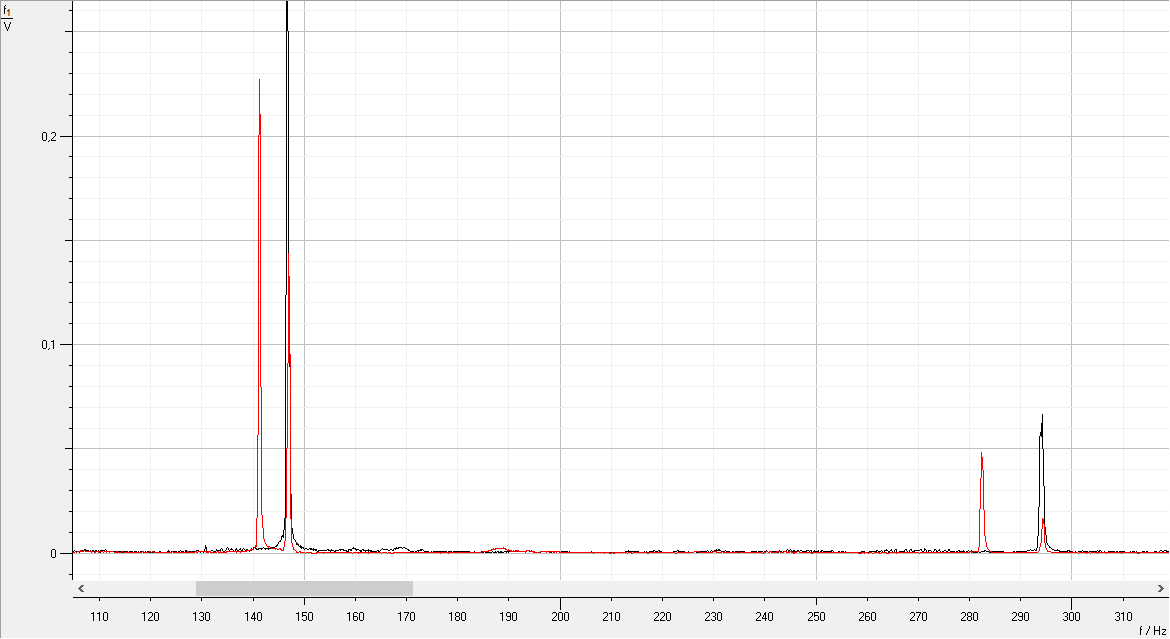
\includegraphics[scale=0.5]{Bilder/Verstimmt_vs_3_stimmen.png}
\caption{Verstimmte D-Saite in rot gegen den dritten Stimmversuch in schwarz. Bei den Peaks der Grundschwingung und der 1. Oberschwingung ist keine Schwebung erkennbar.}
\end{figure}

Die D-Saite sollte nun also wieder gut gestimmt sein, was auch mit dem Stimmgerät überprüft wurde. Das Stimmen über die Schwebung war also erfolgreich.

\section{Bestimmung der Materialeigenschaften der Saiten}
\subsection{Versuchsbeschreibung}
Für den Grundton $f$ einer Gitarrensaite gilt:
\begin{equation}
f=\frac{1}{2}\sqrt{\frac{T}{\mu}}\cdot \frac{1}{l}
\label{Grundgleichung Gitarre f gegen l}
\end{equation}
mit der Saitenspannung T in N, dem Massebelag $\mu$ in $\frac{kg}{m}$ und der Länge der Saite $l$ in m.
In diesem Versuch wird dieselbe Saite bei unterschiedlichen Längen angeschlagen und die entsprechende Frequenz gemessen. Trägt man dann $f$ gegen $\frac{1}{l}$ auf erhält man aus der Steigung $m=\frac{1}{2}\sqrt{\frac{T}{\mu}}$ einen Wert für das Verhältnis von $T$ und $\mu$, das mit den Herstellerangaben verglichen werden sollte.\newline Wir haben uns hier auf die Vermessung der Materialeigenschaften der A-Saite beschränkt.

\subsection{Versuchsaufbau und Durchführung}
Der Versuch wurde genau wie der erste Versuch mit der Gitarre aufgebaut. \newline
Zur Vermessung der Frequenz bei unterschiedlichen Längen wurde die A-Saite zuerst leer, dann im 2ten, 4ten, 6ten, 8ten und 10ten Bund jeweils 3 mal angeschlagen. Die Messung mit Mikrofon und Cassy selbst erfolgte wie im Teilversuch zuvor.
Die Frequenzen selbst wurden mittels Fast-Fourier-Transformation und Peakschwerpunktsberechnung bestimmt. Die jeweils drei Frequenzen wurden dann gemittelt und über Gleichung (\ref{sigmean}) der Fehler auf den Mittelwert bestimmt.
\newline
Die Länge der Anschlagpunkte wurden mit dem Maßband vermessen.\newline

\begin{table}[H]\centering
\caption{Messwerterfassungseinstellungen}
\begin{tabular}{c|c}
Parameter & Einstellung \\ 
\hline
Messintervall & 500 $\mu$s \\ 
Anzahl Messwerte & 10000 \\ 
Messdauer & 5s \\ 
Trigger & 0.3V \\ 
\end{tabular} 
\end{table}

\subsection{Versuchsauswertung}

\subsubsection{Rohdaten}
\begin{table}[H]\centering
\caption{Längenmessungen der Anschlagpunkte}
\begin{tabular}{c|c|c}
$L_0$ & 64.9 cm & Leere Saite\\ 
$L_1$ & 54.6 cm & 2. Bund \\ 
$L_2$ & 51.5 cm & 4. Bund \\ 
$L_3$ & 45.9 cm & 6. Bund \\ 
$L_4$ & 40.9 cm & 8. Bund \\ 
$L_5$ & 36.4 cm & 10. Bund \\ 
\end{tabular} 
\end{table}
Die Messung am 2. Bund wurde in der Auswertung ausgelassen, da die Längenmessung offenbar fehlgeschlagen ist. Die Abstände vom Steg zu den jeweiligen Bünden wurden mit dem Maßband bestimmt, daher haben wir den Fehler auf:
\begin{equation*}
\sigma_L=1 mm
\end{equation*}
abgeschätzt.


\begin{table}[H]\centering
\caption{Frequenzmessung bei unterschiedlichen Längen}
\begin{tabular}{c|cccccc}
 & $L_0$ & $L_1$ & $L_2$ & $L_3$ & $L_4$ & $L_5$ \\ 
\hline 
$f_1$ & 110.16 & 123.80 & 138.98 & 156.03 & 174.60 & 194.42 \\ 
$f_2$ & 110.20 & 123.79 & 139.04 & 155.69 & 174.31 & 196.00 \\ 
$f_3$ & 110.24 & 123.79 & 138.83 & 155.96 & 174.46 & 195.97 \\ 
$\bar{f}$ & 110.20 & 123.79 & 138.95 & 155.89 & 174.46 & 195.46 \\ 
$\sigma_{\bar{f}}$ & 0.02 & 0.00 & 0.06  & 0.10 & 0.08  & 0.52  \\ 
\end{tabular}
\newline 
Angaben in Hz
\end{table}
$~$\newline
Der Fehler auf die Frequenz ist bei der Vermessung des 2. Bunds sehr klein (ungerundet: $\sigma_{\bar{f_1}}=0.0033$). Dieser Wert wurde aber schon wegen der Längenmessung weggelassen.
$~$\newline
$~$\newline
Für die von uns vermessene A-Saite gilt laut Skript:
\begin{equation*}
\mu_{lit}=3.4095 \cdot 10^{-3} \frac{kg}{m}, \hspace{1cm}
T_{lit}=68.04 N.
\end{equation*}
Für die Steigung ist also ein Wert von
\begin{equation}
m_{lit}=\frac{1}{2}\sqrt{\frac{T_{lit}}{\mu_{lit}}}=70.633 \frac{m}{s}
\label{Herstellerangabe Gitarre}
\end{equation}
zu erwarten.
\subsubsection{Transformation der Rohdaten}
Die nun bestimmten gemittelten Frequenzen können jetzt mit ihren Fehlern gegen die jeweiligen Längen mit ihren Fehlern aufgetragen werden.
\begin{figure}[H]\centering
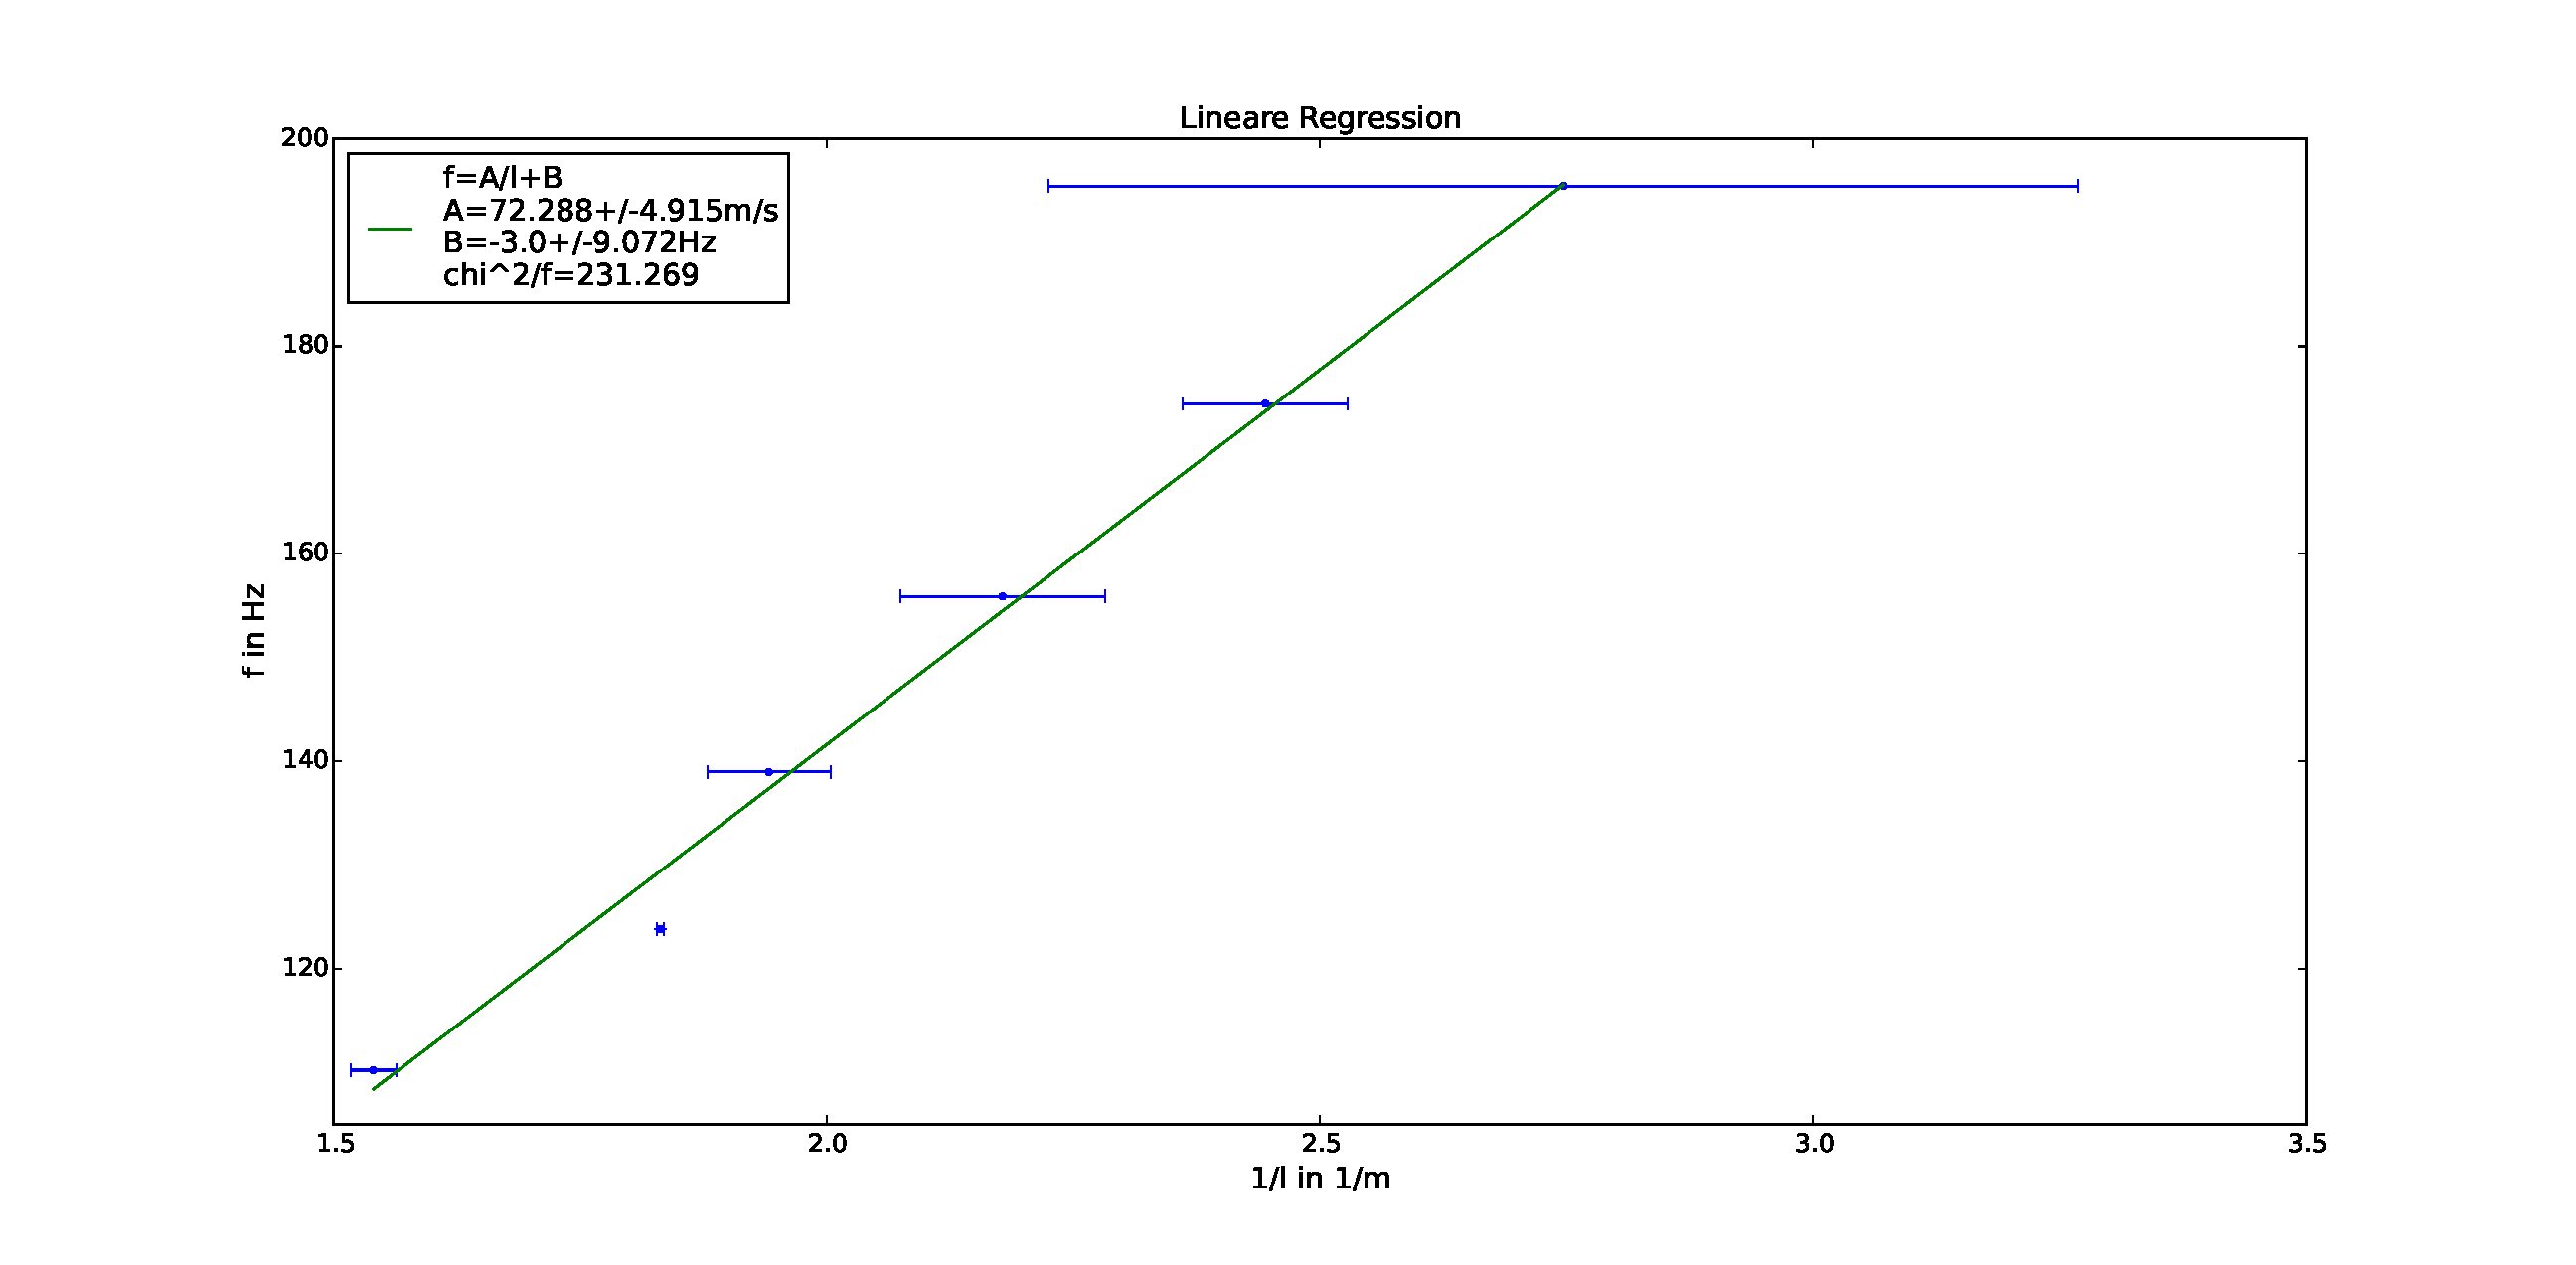
\includegraphics[scale=0.4]{Bilder/lin_reg_mit.eps}
\caption{Lineare Regression aller Werte. Der 2. Wert ist ein deutlicher Ausreißer und wurde daher im Folgenden weggelassen.}
\end{figure}

\begin{figure}[H]
\centering
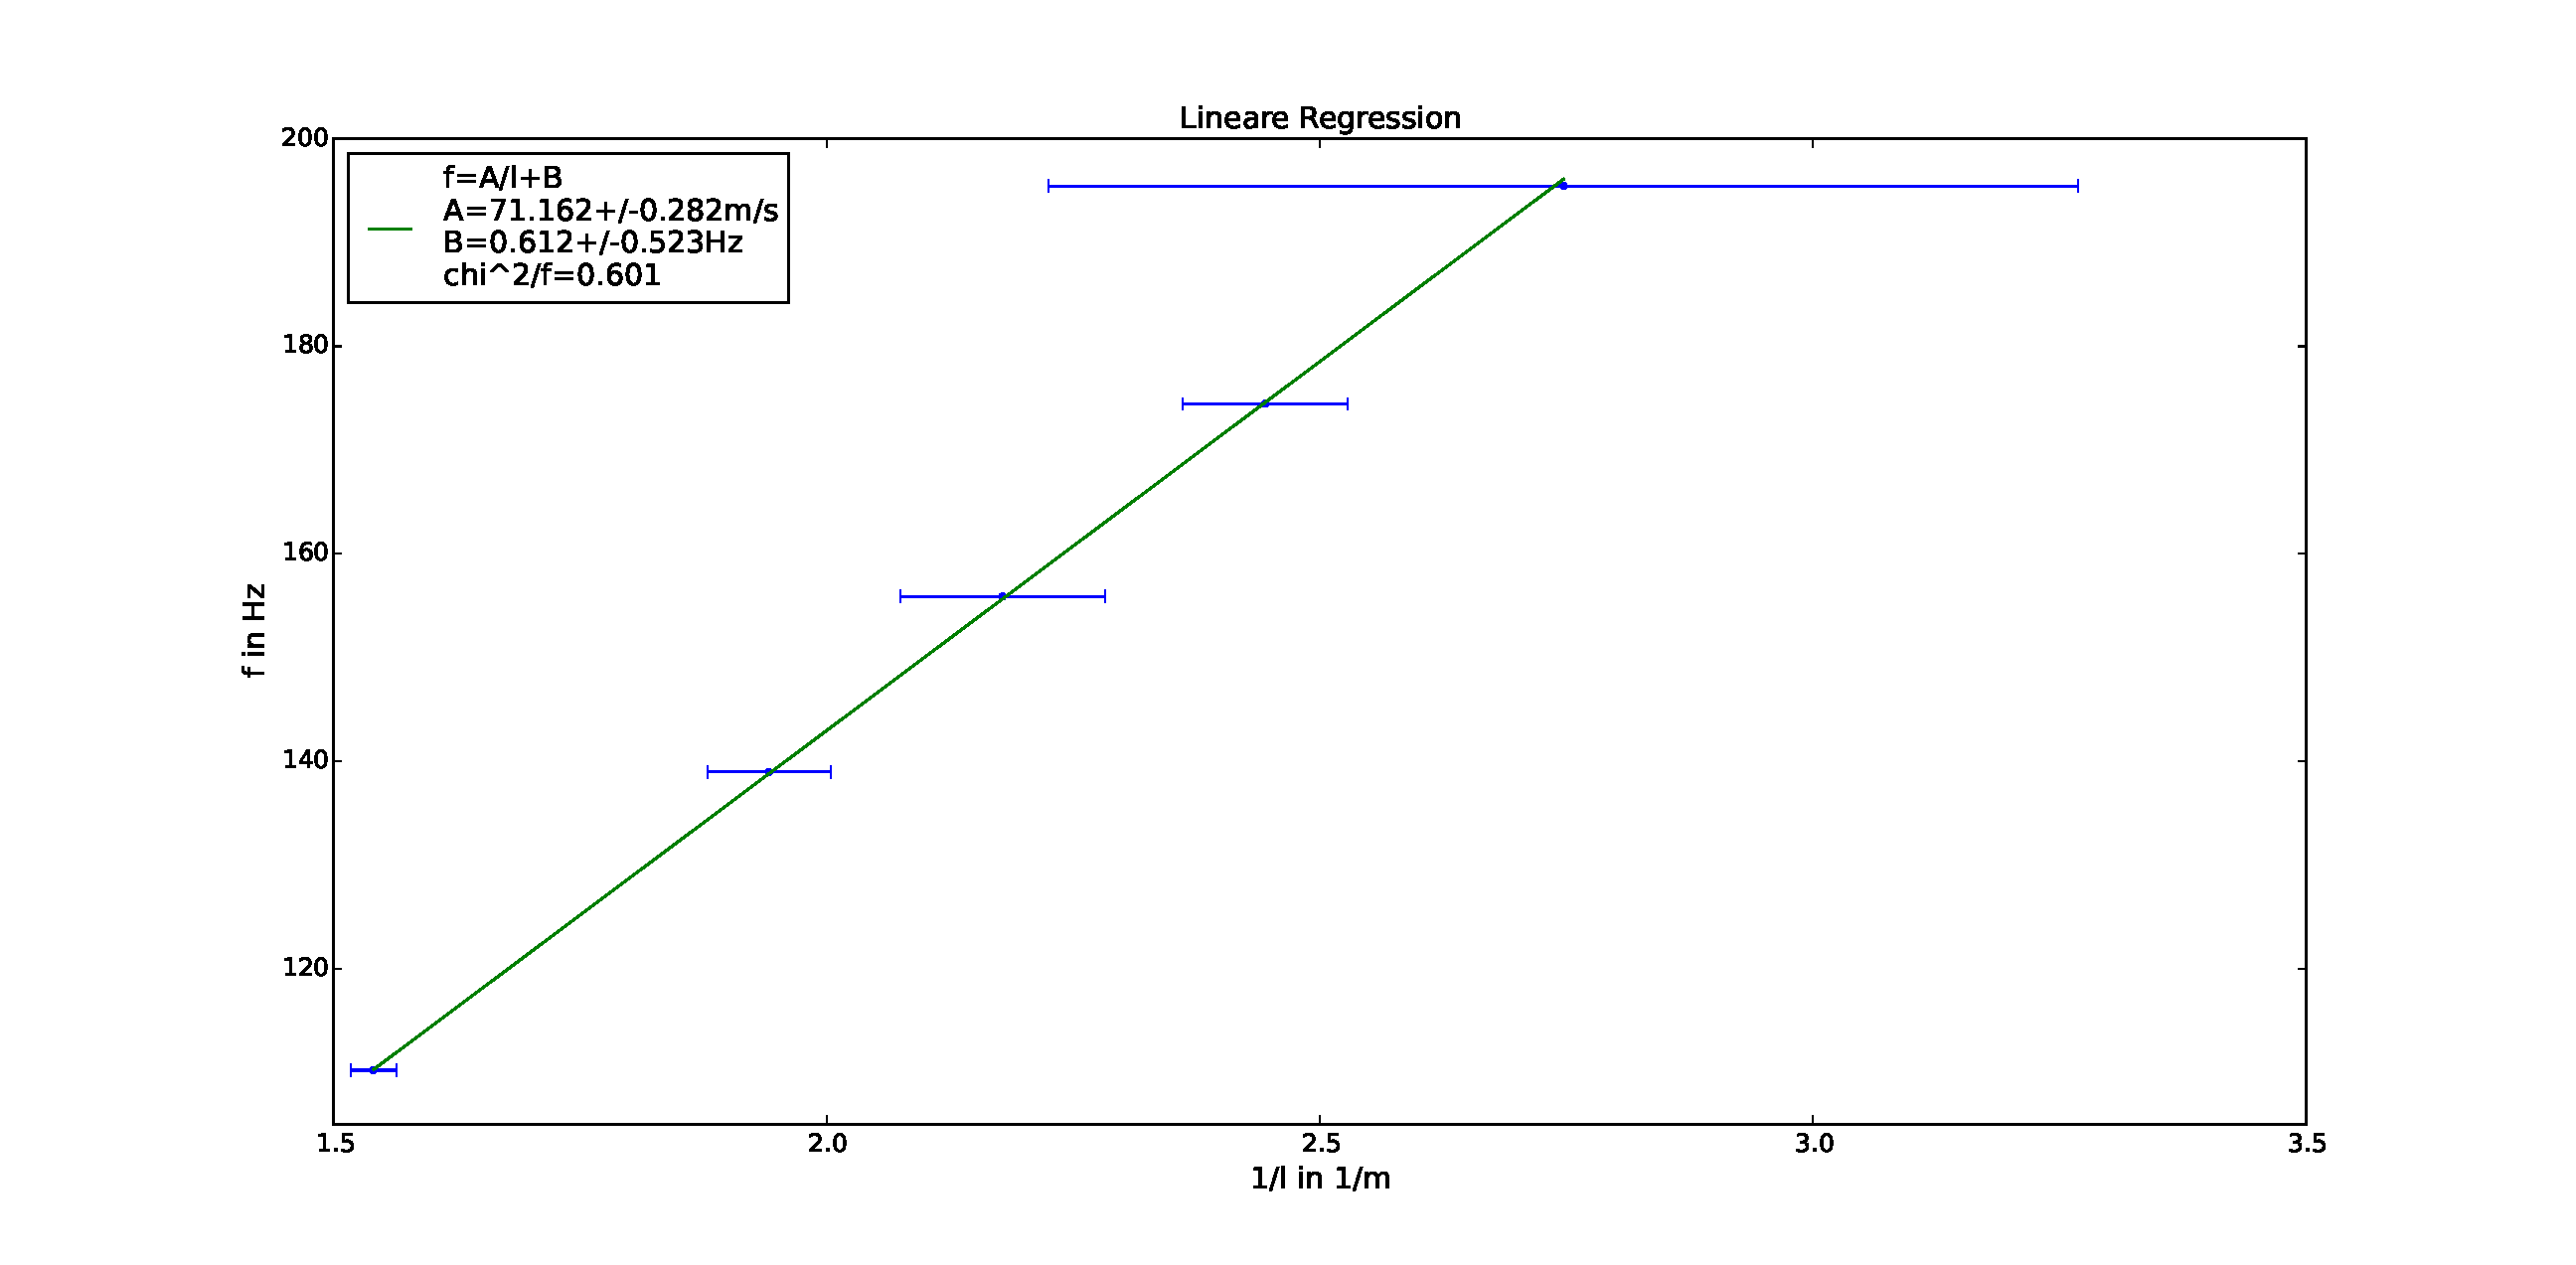
\includegraphics[scale=0.4]{Bilder/lin_reg_ohne.eps}
\caption{Lineare Regression ohne den zweiten Wert. Der Fehler steigt mit $\frac{1}{l}$, da die Saite bei kürzerer Länge stärker gedämpft ist und nicht so lange schwingt.}
\end{figure}


\begin{figure}[H]
\centering
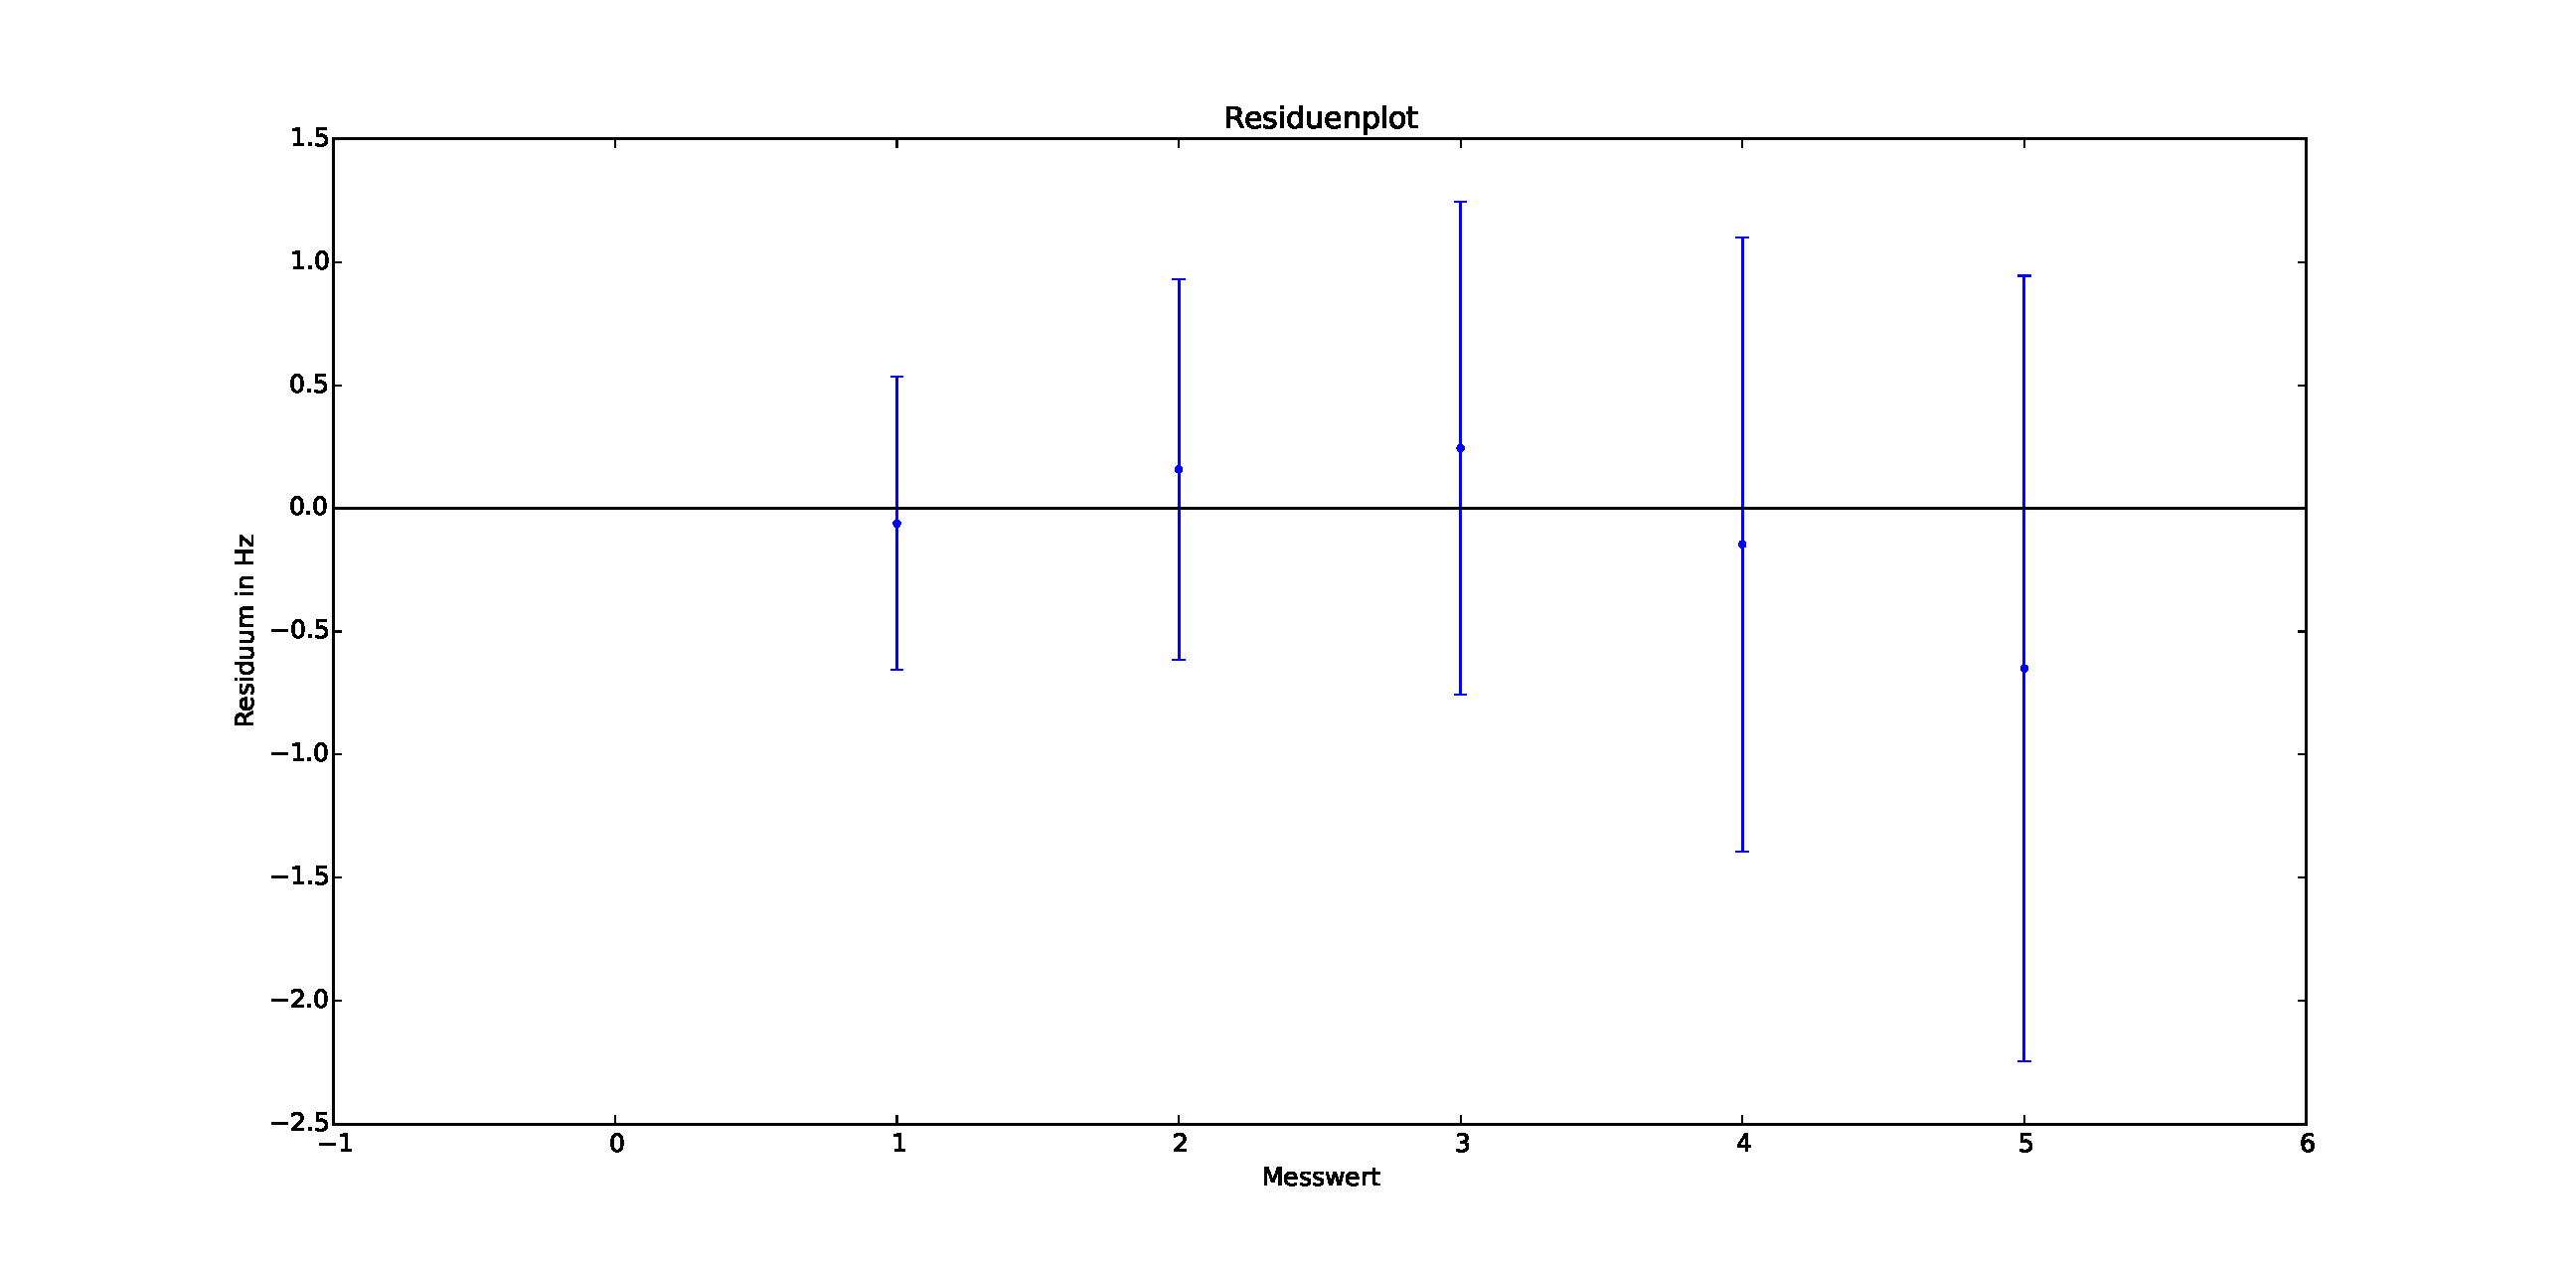
\includegraphics[scale=0.4]{Bilder/lin_reg_ohne_residuum.eps}
\caption{Residuenplot ohne den zweiten Wert. Der Residuenplot zeigt keine Systematik und alle Messwerte schneiden mit ihren Fehlern die Null-Linie.}
\end{figure}

Ergebnis der Linearen Regression:
\begin{align*}
A = m &= 71.162 \pm 0.282 \frac{m}{s}  \\
B &= 0.612 \pm 0.523 Hz \\
\frac{\chi^2}{f}&=0.601
\end{align*}

Zum Vergleich (siehe Gleichung \ref{Herstellerangabe Gitarre}):
\begin{equation}
m_{lit}=70.633 \frac{m}{s}
\end{equation}

\subsubsection{Fazit}
Der Wert aus den Herstellerangaben liegt im Bereich von 2 Standardabweichungen unter dem gemessenen Wert. Dies ist darauf zurückzuführen, dass die Gitarre im Laufe der Zeit abgenutzt wurde und daher der Massebelag mittlerweile eher kleiner ist als bei der Herstellerangabe für die neue Saite. \newline
Der gemessene y-Achsenabschnitt von $B = 0.612 \pm 0.523$ Hz liegt mit seinem Fehler nahe genug an dem erwarteten Wert von 0 (siehe Gleichung \ref{Grundgleichung Gitarre f gegen l}).
\newline
Das $\frac{\chi^2}{f}$ von 0.601 lässt zwar auf einen leicht überschätzten Fehler schließen, ist aber noch in einem vertretbaren Bereich.
\section{Aufnahme eines Frequenzspektrums}
\subsection{Versuchsbeschreibung}
Bei Grundschwingungen (1. Harmonische) befinden sich die Knoten an den Saiten-Enden. Neben der Grundschwingung bilden sich aber auch weitere sogenannte Oberschwingungen aus, die an den Enden ebenfalls Knoten bilden. Für die Wellenlängen dieser so genannten  n-ten Harmonischen gilt:
\begin{equation}
\lambda_n=	\frac{2L}{n}
\end{equation}
Für n=1 ergibt sich die Grundschwingung für n = 2 die 1. Oberschwingung für n = 3 die 2. Oberschwingung und so weiter.
\newline
\begin{figure}[H]
\centering
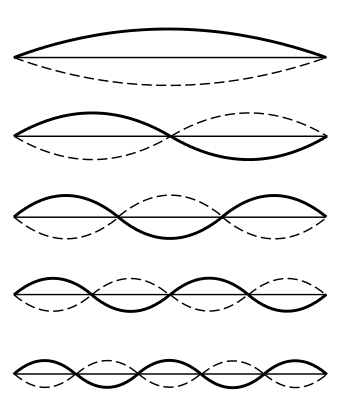
\includegraphics[scale=1]{Bilder/Harmonische.png}
\caption{Stehende Welle und deren Harmonische bis n = 5.}
\end{figure}

Schlägt man die Saite im Abstand $d=\frac{L}{n}$ an, fehlen die n-te Harmonische und ihre Vielfachen, da sich dort kein Knoten bilden kann.

In diesem Versuch sollte das Frequenzspektrum der D-Saite einer Gitarre, die an verschiedenen Abständen angeschlagen wurde auf das oben beschriebene Verhalten untersucht werden.

\subsection{Versuchsaufbau und Durchführung}
Der Aufbau ist derselbe wie in den anderen Versuchen zur Gitarre. 

\begin{table}[H]\centering
\caption{Messparameter für Aufnahme des Frequenzspektrums der D-Saite.}
\begin{tabular}{c|c}
Parameter & Einstellungen \\ 
\hline
Messintervall & 100 $\mu s$ \\ 
Anzahl Messwerte & 16000 \\ 
Messdauer & 1.6s \\ 
Trigger & 0.3V \\ 
\end{tabular}
\end{table}

Als Erstes wurde die D-Saite in der Mitte angeschlagen.
\begin{figure}[H]
\centering
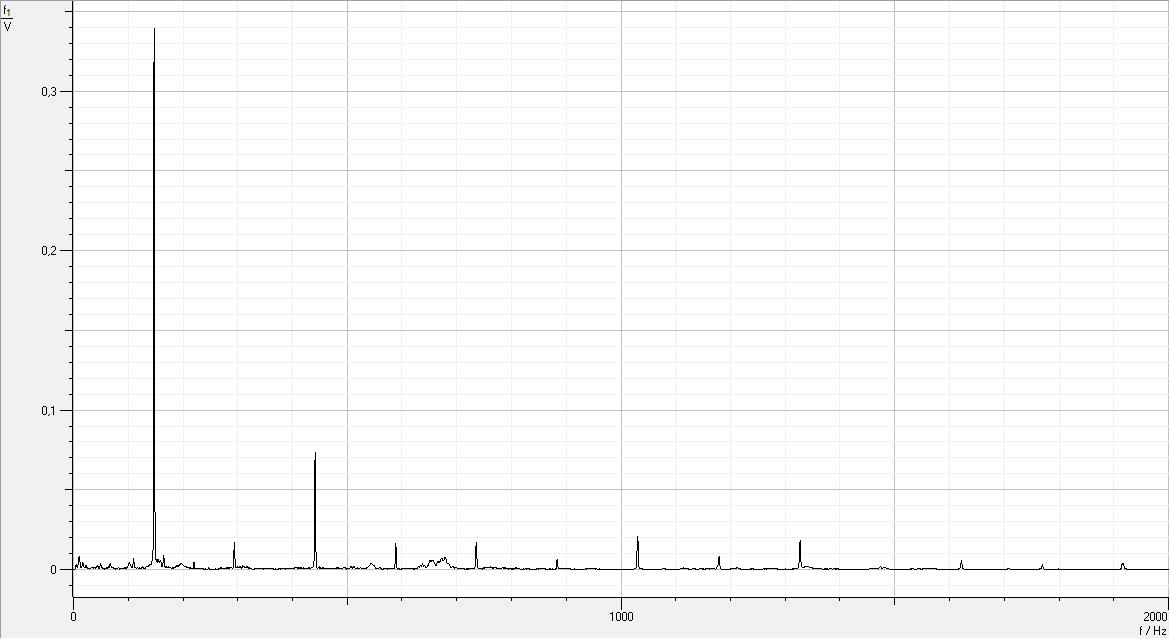
\includegraphics[scale=0.45]{Bilder/Spektrum_Mitte.png}
\caption{Grundfrequenz von 147,03 Hz ist deutlich erkennbar. Nur jede zweite Schwingung ist ausgeprägt.}
\end{figure}

Zum Vergleich wurde die Saite sehr weit oben am Hals angeschlagen.
\begin{figure}[H]
\centering
\includegraphics[scale=0.45]{Bilder/Spektrum_oben.png}
\caption{Die Amplituden fallen bis zur 6. Harmonischen stetig ab.}
\end{figure}

\subsection{Fazit}
Wie in den gezeigten Abbildungen zu sehen ist, konnten wir die Theorie, dass die n-ten Harmonischen fehlen, wenn man die Saite an einem Abstand von $d=\frac{L}{n}$ anschlägt, bestätigen.

\end{document}